% This is samplepaper.tex, a sample chapter demonstrating the
% LLNCS macro package for Springer Computer Science proceedings;
% Version 2.20 of 2017/10/04
%
\documentclass[runningheads]{llncs}
%
\usepackage{graphicx}
\usepackage[appendix=strip]{apxproof}%default
\graphicspath{
  {fig/}
  {fig/exp1/}
  {fig/fig1/}
  {fig/turu/}
}%%画像のパス.末尾は'/'で終わること
%% \usepackage[appendix=append]{apxproof}%default
%% \usepackage[appendix=inline]{apxproof}%default

% Used for displaying a sample figure. If possible, figure files should
% be included in EPS format.
%
% If you use the hyperref package, please uncomment the following line
% to display URLs in blue roman font according to Springer's eBook style:
% \renewcommand\UrlFont{\color{blue}\rmfamily}

%%%%%%%%%%%%%%%%%%%%%%%%%%%%%%%%%%%%%%%
%%% macros
%% %%% config.tex

%%======================================
\usepackage{graphicx}
%% \usepackage{amsmath,amssymb}
%% \usepackage{mathtools}
%% \mathtoolsset{showonlyrefs=false} %% 参照している式参照のみ表示
%% \mathtoolsset{showonlyrefs=true} %% 参照している式参照のみ表示
%% \usepackage{cite}
\usepackage{caption}    %%for subfigure
\usepackage[skip=0.5ex]{subcaption} %%for subfigure
\captionsetup{aboveskip=0.0\baselineskip}
\captionsetup{belowskip=0.0\baselineskip}
%%%
%%\usepackage{titlesec}
%% \titlespacing*{\section}{0pt}{5.5ex plus 1ex minus .2ex}{4.3ex plus .2ex}
%% \titlespacing*{\subsection}{0pt}{5.5ex plus 1ex minus .2ex}{4.3ex plus .2ex}

%%% table
%% \usepackage{multirow}
\usepackage{booktabs}
\usepackage{array}

% private macros by others 
\usepackage{url}
\usepackage{bm}
\usepackage{textcomp}%%for cent
%\usepackage[margin=1.75in]{geometry}
%\usepackage[margin=1.0in]{geometry}
%% \usepackage{subfig}
%% \usepackage{natbib}

%%% private %%%%%%%%%%%%%%%%%%%%%%%%%%%%%%%%%%%%%

%% private macros by arim@ist
%%% jsvmac.tex
%%% macros from a subset of jsv1.sty 

%%% from jsv1.sty

% Write multichar identifier names using \id in either mathmode or text;
% For ex, $\id{high}(x)$ is an expression using the \id{high} function.
% Use ``\ '' if a space is desired, as in math mode.
\def\id#1{\ensuremath{\mathit{#1}}}
\let\idit=\id
\def\idbf#1{\ensuremath{\mathbf{#1}}}
\def\idrm#1{\ensuremath{\mathrm{#1}}}
\def\idtt#1{\ensuremath{\mathtt{#1}}}
\def\idsf#1{\ensuremath{\mathsf{#1}}}
\def\idcal#1{\ensuremath{\mathcal{#1}}}  % Use with capital letter args only
\def\idsc#1{\ensuremath{\textsc{#1}}} % added by arim

%%% end jsv1.sty

%%% EOF

%%\input{arimmacro} %%privatemacro


%%%%%%%%%%%%%%%%%%%%%%%%%%%%%%%%%%%%%%%%
%%xsavebox
\usepackage{xsavebox}

%%%%%%%%%%%%%%%%%%%%%%%%%%%%%%%%%%%%%%%%%
%%% above and below float figure table
\setlength\intextsep{0.5\baselineskip}
\setlength\abovecaptionskip{0.0\baselineskip}
\setlength\belowcaptionskip{0.5\baselineskip}
%% \setlength\intextsep{18pt}

%%%%%%%%%%%%%%%%%%
%% latex native savebox and lrbox
\newenvironment{savethm}[1]{\begin{lrbox}{#1}\begin{minipage}[t]{1.0\textwidth}}{\end{minipage}\end{lrbox}}

\newcommand{\putthm}[1]{
%% \smallskip
\noindent 
\usebox{#1}
\medskip}

%%sample
%% \newsavebox{\thmbox}
%% \begin{lrbox}{\thmbox}
%% \begin{minipage}[t]{1.0\textwidth}
%% \begin{theorem}\label{thm:algbwt:main}
%% ....
%% \end{theorem}
%% \end{minipage}
%% \end{lrbox}


%% \putthm{\thmbox}


%%%%%%%%%%%%%%%%%%




%%%%%%%%%%%%%%%%%%%%%%%%%%%%%%%%%%%%%%%%
%%comment out a paragraph
\newsavebox{\cmbox}
\newenvironment{commbox}{
  \begin{lrbox}{\cmbox}
    \begin{minipage}{.9\textwidth}
}{\end{minipage}
  \end{lrbox}
  %\framebox{\usebox{\cmbox}}
}


%%%%%%%%%%%%%%%%%%%%%%%%%%%%%%%%%%%%%%%%
% %%% empty environment 
% \newenvironment{myempty}{\begin{commbox}}{\end{commbox}}
% %%% proof environment 
% \newenvironment{myproof}{\begin{proof}}{\end{proof}} %default
% \newenvironment{myfullproof}{\begin{proof}}{\end{proof}} %default
% \newenvironment{myfullproofempty}{\begin{myempty}}{\end{myempty}} %default

%% replace an enviroment #1 with #2
\newcommand{\myenvironmentreplace}[2]{\renewenvironment{#1}{\begin{#2}}{\end{#2}}}

%% claim %%
\newenvironment{myclaim}[1][]{\bgroup\parskip=0mm\par (\textit{Claim{#1}})}{(\textit{End of Claim})\par\egroup}  
\newenvironment{proofofclaim}{\bgroup\parindent=1em\parskip=0mm\par (\textit{Proof for the claim})}{(\textit{End of the proof for the claim})\par\egroup}  
\newenvironment{proofofclaimempty}{\begin{myempty}}{\end{myempty}}

%% \newenvironment{proofofclaim}{\bgroup\parskip=0mm\par (Proof for the claim)}{(End of the proof for the claim)\par\egroup}  


%%%%%%%%%%%%%%%%%%%%%%%%%%%%%%%%%%%%%%%%

% %% switch catcode of '&' between 4 and 9
% \newenvironment{inalign}{\begin{math}\catcode`&=9}{\catcode`&=4\end{math}}

%%%%%%%%%%%%%%%%%%%%%%%%%%%%%%%%%%%%%%%%

% lipics predefined

%% send a proof to the appendix
\newtheorem{definition}{Definition}
\newtheorem{theorem}{Theorem}
\newtheorem{lemma}[theorem]{Lemma}
\newtheorem{proposition}{Proposition}
\newtheorem{corollary}[theorem]{Corollary}
\newtheorem{remark}{Remark}
\newtheorem{fact}{Fact}
\newtheorem{condition}{Condition}

% \newtheorem{example}[example]{Example}[section]
% \newtheorem{conjecture}{Conjecture}
% %% dammy
%%%%%%%%%%%%%%%%%%%%%%%%%%%%%%%%%%%%%%%%

%%% cleveref
\usepackage{cleveref}
\crefname{section}{Sec.}{Sections}
\crefname{chapter}{Chapter}{Chapters}
%%
\crefname{algorithm}{Algorithm}{Algorithms}
\crefname{table}{Table}{Tables}
\crefname{figure}{Fig.}{Figures}
%% 
\crefname{definition}{Definition}{Definitions}
\crefname{lemma}{Lemma}{Lemmas}
\crefname{proposition}{Prop.}{Propositions}
\crefname{theorem}{Theorem}{Theorems}
\crefname{remark}{Remark}{Remarks}
\crefname{fact}{Fact}{Facts}
\crefname{condition}{Condition}{Conditions}
\crefname{problem}{Problem}{Problems}
\crefname{observation}{Observation}{Observations}
%% \crefname{lemma}{Lemma}{Lemmas}
\crefname{equation}{Eq.}{Equations}
%%% fix of a bug in Algorithm
\newcommand{\aref}[1]{Algorithm\kern0.25em\ref{#1}} 
%%%%%%

% %% send a proof to the appendix
\usepackage{apxproof}
% \newtheoremrep{definition}{Definition}[section]
\newtheoremrep{lemma}[theorem]{Lemma}[section]
\newtheoremrep{proposition}[proposition]{Proposition}[section]
\newtheoremrep{theorem}[theorem]{Theorem}[section]
\newtheoremrep{corollary}[theorem]{Corollary}[section]
% \newtheoremrep{remark}[theorem]{Remark}

%% \newtheoremrep{example}[example]{Example}[section]
%% \newtheoremrep{conjecture}{Conjecture}
%% %% dammy
%% \newcommand{\resetrep}{}
%% rest 
%% \newcommand{\resetreptext}{{\rm\textsf{in draft}}}
%% \newcommand{\getfollow}[1][{}]{{\rm\textsf{(*{#1})}}\ }

%% \newcommand{\resetrep}{%% resetting all rep-style environments
%% %% \renewenvironment{lemmarep}{\begin{lemma}\getfollow}{\end{lemma}}
%% \renewenvironment{lemmarep}{\begin{lemma}\getfollow}{\end{lemma}}
%% \renewenvironment{propositionrep}{\begin{proposition}\getfollow}{\end{proposition}}
%% \renewenvironment{theorem}{\begin{theorem}\getfollow}{\end{theorem}}
%% \renewenvironment{corollaryrep}{\begin{corollary}\getfollow}{\end{corollary}}
%% \renewenvironment{examplerep}{\begin{example}\getfollow}{\end{example}}
%% \renewenvironment{remarkrep}{\begin{remark}\getfollow}{\end{remark}}
%% \renewenvironment{conjecturerep}{\begin{conjecture}\getfollow}{\end{conjecture}}
%% \renewenvironment{toappendix}{}{}
%% }

%%%%% 
\newenvironment{statement}[1]{\begin{trivlist}\item[]$\blacktriangleright\:$\textbf{#1}\ }{\end{trivlist}}
\newenvironment{notoappendix}{}{} %% the empty version of toappendix

%%%%%%%%%%%%%%%%%%%%%%%%%%%%%%%%%%%%%%%%%
%% enumitem: smart enumerate and itemize
%% the vspace above list = \topsep + \parskip + \partopsep
%% the vspace between items = \itemsep + \Parsep 
%% the vspace between paragraphs = \Parsep 
\usepackage[inline,shortlabels]{enumitem} %enumerate
\setlist{noitemsep}
\setlist{%
topsep = 0.25\baselineskip,
parsep = 0.125\baselineskip
}%exp
\setlist[enumerate]{ labelsep=.25pc, leftmargin=1.5pc } 
%% \setlist[enumerate]{ labelsep=.25pc, leftmargin=1.5pc } 
\setlist[enumerate,1]{ label= (\arabic*), ref=\arabic*}
\setlist[enumerate,2]{ label= (\roman*),ref  = \roman*}
\setlist[enumerate,3]{ label= (\alph*), ref  = (\alph*)}
%\setlist[itemize]{ leftmargin=1.5pc }
\setlist[description]{ font=\sffamily\bfseries }
%% end macros
%%% switch
%% \newenvironment{myenumerate}{\begin{enumerate}}{\end{enumerate}}
\newenvironment{myenumerate}{\begin{enumerate*}}{\end{enumerate*}}
%% end macros

%%

%% %% 目次のハイパーリンク: 印刷時は念の為コメントアウト(本来出ない)
%% \usepackage[%
%% %dvipdfmx,%
%% colorlinks=true,%
%% linkcolor=blue,%
%% anchorcolor=black,%
%% citecolor=blue,%
%% urlcolor=blue%
%% ]{hyperref} %注意:パッケージの最後に読み込むこと

%%%%

%% EOF

%%% config.tex

%%======================================
\usepackage{graphicx}
%% \usepackage{amsmath,amssymb}
%% \usepackage{mathtools}
%% \mathtoolsset{showonlyrefs=false} %% 参照している式参照のみ表示
%% \mathtoolsset{showonlyrefs=true} %% 参照している式参照のみ表示
%% \usepackage{cite}
\usepackage{caption}    %%for subfigure
\usepackage[skip=0.5ex]{subcaption} %%for subfigure
\captionsetup{aboveskip=0.0\baselineskip}
\captionsetup{belowskip=0.0\baselineskip}
%%%
%%\usepackage{titlesec}
%% \titlespacing*{\section}{0pt}{5.5ex plus 1ex minus .2ex}{4.3ex plus .2ex}
%% \titlespacing*{\subsection}{0pt}{5.5ex plus 1ex minus .2ex}{4.3ex plus .2ex}

%%% table
%% \usepackage{multirow}
\usepackage{booktabs}
\usepackage{array}

% private macros by others 
\usepackage{url}
\usepackage{bm}
\usepackage{textcomp}%%for cent
%\usepackage[margin=1.75in]{geometry}
%\usepackage[margin=1.0in]{geometry}
%% \usepackage{subfig}
%% \usepackage{natbib}

%%% private %%%%%%%%%%%%%%%%%%%%%%%%%%%%%%%%%%%%%

%% private macros by arim@ist
%%% jsvmac.tex
%%% macros from a subset of jsv1.sty 

%%% from jsv1.sty

% Write multichar identifier names using \id in either mathmode or text;
% For ex, $\id{high}(x)$ is an expression using the \id{high} function.
% Use ``\ '' if a space is desired, as in math mode.
\def\id#1{\ensuremath{\mathit{#1}}}
\let\idit=\id
\def\idbf#1{\ensuremath{\mathbf{#1}}}
\def\idrm#1{\ensuremath{\mathrm{#1}}}
\def\idtt#1{\ensuremath{\mathtt{#1}}}
\def\idsf#1{\ensuremath{\mathsf{#1}}}
\def\idcal#1{\ensuremath{\mathcal{#1}}}  % Use with capital letter args only
\def\idsc#1{\ensuremath{\textsc{#1}}} % added by arim

%%% end jsv1.sty

%%% EOF

%%\input{arimmacro} %%privatemacro


%%%%%%%%%%%%%%%%%%%%%%%%%%%%%%%%%%%%%%%%
%%xsavebox
\usepackage{xsavebox}

%%%%%%%%%%%%%%%%%%%%%%%%%%%%%%%%%%%%%%%%%
%%% above and below float figure table
\setlength\intextsep{0.5\baselineskip}
\setlength\abovecaptionskip{0.0\baselineskip}
\setlength\belowcaptionskip{0.5\baselineskip}
%% \setlength\intextsep{18pt}

%%%%%%%%%%%%%%%%%%
%% latex native savebox and lrbox
\newenvironment{savethm}[1]{\begin{lrbox}{#1}\begin{minipage}[t]{1.0\textwidth}}{\end{minipage}\end{lrbox}}

\newcommand{\putthm}[1]{
%% \smallskip
\noindent 
\usebox{#1}
\medskip}

%%sample
%% \newsavebox{\thmbox}
%% \begin{lrbox}{\thmbox}
%% \begin{minipage}[t]{1.0\textwidth}
%% \begin{theorem}\label{thm:algbwt:main}
%% ....
%% \end{theorem}
%% \end{minipage}
%% \end{lrbox}


%% \putthm{\thmbox}


%%%%%%%%%%%%%%%%%%




%%%%%%%%%%%%%%%%%%%%%%%%%%%%%%%%%%%%%%%%
%%comment out a paragraph
\newsavebox{\cmbox}
\newenvironment{commbox}{
  \begin{lrbox}{\cmbox}
    \begin{minipage}{.9\textwidth}
}{\end{minipage}
  \end{lrbox}
  %\framebox{\usebox{\cmbox}}
}


%%%%%%%%%%%%%%%%%%%%%%%%%%%%%%%%%%%%%%%%
% %%% empty environment 
% \newenvironment{myempty}{\begin{commbox}}{\end{commbox}}
% %%% proof environment 
% \newenvironment{myproof}{\begin{proof}}{\end{proof}} %default
% \newenvironment{myfullproof}{\begin{proof}}{\end{proof}} %default
% \newenvironment{myfullproofempty}{\begin{myempty}}{\end{myempty}} %default

%% replace an enviroment #1 with #2
\newcommand{\myenvironmentreplace}[2]{\renewenvironment{#1}{\begin{#2}}{\end{#2}}}

%% claim %%
\newenvironment{myclaim}[1][]{\bgroup\parskip=0mm\par (\textit{Claim{#1}})}{(\textit{End of Claim})\par\egroup}  
\newenvironment{proofofclaim}{\bgroup\parindent=1em\parskip=0mm\par (\textit{Proof for the claim})}{(\textit{End of the proof for the claim})\par\egroup}  
\newenvironment{proofofclaimempty}{\begin{myempty}}{\end{myempty}}

%% \newenvironment{proofofclaim}{\bgroup\parskip=0mm\par (Proof for the claim)}{(End of the proof for the claim)\par\egroup}  


%%%%%%%%%%%%%%%%%%%%%%%%%%%%%%%%%%%%%%%%

% %% switch catcode of '&' between 4 and 9
% \newenvironment{inalign}{\begin{math}\catcode`&=9}{\catcode`&=4\end{math}}

%%%%%%%%%%%%%%%%%%%%%%%%%%%%%%%%%%%%%%%%

% lipics predefined

%% send a proof to the appendix
\newtheorem{definition}{Definition}
\newtheorem{theorem}{Theorem}
\newtheorem{lemma}[theorem]{Lemma}
\newtheorem{proposition}{Proposition}
\newtheorem{corollary}[theorem]{Corollary}
\newtheorem{remark}{Remark}
\newtheorem{fact}{Fact}
\newtheorem{condition}{Condition}

% \newtheorem{example}[example]{Example}[section]
% \newtheorem{conjecture}{Conjecture}
% %% dammy
%%%%%%%%%%%%%%%%%%%%%%%%%%%%%%%%%%%%%%%%

%%% cleveref
\usepackage{cleveref}
\crefname{section}{Sec.}{Sections}
\crefname{chapter}{Chapter}{Chapters}
%%
\crefname{algorithm}{Algorithm}{Algorithms}
\crefname{table}{Table}{Tables}
\crefname{figure}{Fig.}{Figures}
%% 
\crefname{definition}{Definition}{Definitions}
\crefname{lemma}{Lemma}{Lemmas}
\crefname{proposition}{Prop.}{Propositions}
\crefname{theorem}{Theorem}{Theorems}
\crefname{remark}{Remark}{Remarks}
\crefname{fact}{Fact}{Facts}
\crefname{condition}{Condition}{Conditions}
\crefname{problem}{Problem}{Problems}
\crefname{observation}{Observation}{Observations}
%% \crefname{lemma}{Lemma}{Lemmas}
\crefname{equation}{Eq.}{Equations}
%%% fix of a bug in Algorithm
\newcommand{\aref}[1]{Algorithm\kern0.25em\ref{#1}} 
%%%%%%

% %% send a proof to the appendix
\usepackage{apxproof}
% \newtheoremrep{definition}{Definition}[section]
\newtheoremrep{lemma}[theorem]{Lemma}[section]
\newtheoremrep{proposition}[proposition]{Proposition}[section]
\newtheoremrep{theorem}[theorem]{Theorem}[section]
\newtheoremrep{corollary}[theorem]{Corollary}[section]
% \newtheoremrep{remark}[theorem]{Remark}

%% \newtheoremrep{example}[example]{Example}[section]
%% \newtheoremrep{conjecture}{Conjecture}
%% %% dammy
%% \newcommand{\resetrep}{}
%% rest 
%% \newcommand{\resetreptext}{{\rm\textsf{in draft}}}
%% \newcommand{\getfollow}[1][{}]{{\rm\textsf{(*{#1})}}\ }

%% \newcommand{\resetrep}{%% resetting all rep-style environments
%% %% \renewenvironment{lemmarep}{\begin{lemma}\getfollow}{\end{lemma}}
%% \renewenvironment{lemmarep}{\begin{lemma}\getfollow}{\end{lemma}}
%% \renewenvironment{propositionrep}{\begin{proposition}\getfollow}{\end{proposition}}
%% \renewenvironment{theorem}{\begin{theorem}\getfollow}{\end{theorem}}
%% \renewenvironment{corollaryrep}{\begin{corollary}\getfollow}{\end{corollary}}
%% \renewenvironment{examplerep}{\begin{example}\getfollow}{\end{example}}
%% \renewenvironment{remarkrep}{\begin{remark}\getfollow}{\end{remark}}
%% \renewenvironment{conjecturerep}{\begin{conjecture}\getfollow}{\end{conjecture}}
%% \renewenvironment{toappendix}{}{}
%% }

%%%%% 
\newenvironment{statement}[1]{\begin{trivlist}\item[]$\blacktriangleright\:$\textbf{#1}\ }{\end{trivlist}}
\newenvironment{notoappendix}{}{} %% the empty version of toappendix

%%%%%%%%%%%%%%%%%%%%%%%%%%%%%%%%%%%%%%%%%
%% enumitem: smart enumerate and itemize
%% the vspace above list = \topsep + \parskip + \partopsep
%% the vspace between items = \itemsep + \Parsep 
%% the vspace between paragraphs = \Parsep 
\usepackage[inline,shortlabels]{enumitem} %enumerate
\setlist{noitemsep}
\setlist{%
topsep = 0.25\baselineskip,
parsep = 0.125\baselineskip
}%exp
\setlist[enumerate]{ labelsep=.25pc, leftmargin=1.5pc } 
%% \setlist[enumerate]{ labelsep=.25pc, leftmargin=1.5pc } 
\setlist[enumerate,1]{ label= (\arabic*), ref=\arabic*}
\setlist[enumerate,2]{ label= (\roman*),ref  = \roman*}
\setlist[enumerate,3]{ label= (\alph*), ref  = (\alph*)}
%\setlist[itemize]{ leftmargin=1.5pc }
\setlist[description]{ font=\sffamily\bfseries }
%% end macros
%%% switch
%% \newenvironment{myenumerate}{\begin{enumerate}}{\end{enumerate}}
\newenvironment{myenumerate}{\begin{enumerate*}}{\end{enumerate*}}
%% end macros

%%

%% %% 目次のハイパーリンク: 印刷時は念の為コメントアウト(本来出ない)
%% \usepackage[%
%% %dvipdfmx,%
%% colorlinks=true,%
%% linkcolor=blue,%
%% anchorcolor=black,%
%% citecolor=blue,%
%% urlcolor=blue%
%% ]{hyperref} %注意:パッケージの最後に読み込むこと

%%%%

%% EOF

% macros.tex

%%%%%%%%%%%%%%%%%%%%%%%%%%%%%%%%%%%%%%%%%
%% reference with [] in environment 
\def\refbox(#1){$\mbox{\bf ({#1}) }$}
\newcommand{\mysubsubsection}[1]{\textbf{#1}.\hspace{0.125em}}%% camera
%% \newcommand{\mysubsection}[1]{\subsection*{#1}}

%% private macros: cdawg
%% class names
\newcommand{\suffix}{\id{Suffix}}
\newcommand{\substr}{\id{Substr}}
\newcommand{\prefix}{\id{Prefix}}
\newcommand{\Suf}{\suffix}
\newcommand{\Substr}{\substr}
\newcommand{\Pref}{\prefix}
%%% 
\newcommand{\lext}[1]{\overleftarrow{#1}} 
\newcommand{\rext}[1]{\overrightarrow{#1}} 
\newcommand{\mext}[1]{\overleftrightarrow{#1}}
\newcommand{\str}{\op{str}}
%%%
\newcommand{\spos}[1][S]{\op{Spos}_{#1}}
\newcommand{\epos}[1][S]{\op{Epos}_{#1}}
\newcommand{\occ}[1][]{\op{Occ}_{#1}}
%% maximal 
\newcommand{\RM}{\sig{RM}}
\newcommand{\LM}{\sig{LM}}
\newcommand{\M}{\sig{M}}
%%%%
\newcommand{\rstate}[1]{[{#1}]_{\equiv_R}}
\newcommand{\lstate}[1]{[{#1}]_{\equiv_L}}
%%%
\newcommand{\BUSA}{\textsf{BUSA}} 
\newcommand{\TDSA}{\textsf{TDSA}} 
\newcommand{\TDBW}{\textsf{TDBW}}
%%%
\newcommand{\MAW}{\idit{MAW}} 
\newcommand{\MUS}{\idit{MUS}} 
\newcommand{\MRW}{\idit{MRW}} 
\newcommand{\MRWK}[1][k]{\mbox{$#1$-\idit{MRW}}}
%%%%
%%% data structures
\newcommand{\stree}{\id{STree}}%exp
\newcommand{\weiner}{\id{Weiner}}%exp
\newcommand{\CDAWG}{\mathit{CDAWG}}
\newcommand{\SA}{\id{SA}}
\newcommand{\ISA}{\id{ISA}}
\newcommand{\BWT}{\id{BWT}}
\newcommand{\LCP}{\id{LCP}}
\newcommand{\LCE}[1][T]{\idrm{LCE}_{#1}}
%%%
\newcommand{\repr}{\op{repr}}
\newcommand{\intr}{\op{SA\textrm{-}Int}}
\newcommand{\lcpmin}{\op{lcpmin}}
%%%%
\newcommand{\set}[1]{\{\kern0.05em#1\kern0.05em\}}
\newcommand{\sete}[1]{\{\kern0.2em#1\kern0.2em\}}
\newcommand{\liste}[1]{[\kern0.2em#1\kern0.2em]}

%%%%
%\newcommand{\mywspace}[1][R]{O(\sigma^2\log e_{#1})}
%% \newcommand{\td}{\idsf{Td}}
%% \newcommand{\bu}{\idsf{Bu}}
%% \newcommand{\fw}{\idsf{Fwd}}
%% \newcommand{\bw}{\idsf{Bwd}}
\newcommand{\td}{\idsf{T}}
\newcommand{\bu}{\idsf{B}}
\newcommand{\fw}{\idsf{F}}
\newcommand{\bw}{\idsf{B}}
\newcommand{\tdfw}{\mbox{\td\fw}}
\newcommand{\tdbw}{\mbox{\td\bw}}
\newcommand{\bufw}{\mbox{\bu\fw}}
\newcommand{\bubw}{\mbox{\bu\bw}}
\newcommand{\tdfwd}{\tdfw}%% obsolute 
\newcommand{\tdbwd}{\tdbw}%% obsolute 
\newcommand{\bufwd}{\bufw}%% obsolute 
\newcommand{\bubwd}{\bubw}%% obsolute 
% %%% 

%%%%%%%%%%%%%%%%%%%%%%%%%%%%%%%%%%%%%%%%%
\usepackage{yhmath}%% for neat wide tilde

%%%%%%%%%%%%%%%%%%%%%%%%%%%%%%%%%%%%%%%%%

%% basis 
\renewcommand{\-}{\mbox{\textit{-}}}

%% symbols
\newcommand{\nat}{\mathbb{N}}
\newcommand{\rat}{\mathbb{R}}
\newcommand{\zat}{\mathbb{Z}}
\renewcommand{\leq}{\leqslant}%override
\renewcommand{\le}{\leqslant}%override
\renewcommand{\preceq}{\preccurlyeq}%override
\newcommand{\rev}{^\fn{rev}}

%% typeface 
\newcommand{\proc}[1]{\mbox{\textsf{#1}}}
\newcommand{\algo}[1]{\mbox{\textsf{#1}}}
\newcommand{\fn}[1]{\ensuremath{\mathrm{#1}}} 
\newcommand{\mb}[1]{\mathbb{#1}}
\newcommand{\name}[1]{\textit{#1}}

\newcommand{\eps}{\varepsilon}
\newcommand{\daller}{\$} %$
\renewcommand{\sharp}{\#} %$
\newcommand{\mathdaller}{\mbox{`$\daller$'}} %$
\newcommand{\centsymbol}{\mbox{\textcentoldstyle}} %$
\DeclareMathOperator{\polylog}{\mathrm{polylog}}

\newcommand{\kw}[1]{\textbf{#1}}
\newcommand{\sig}[1]{\mathcal{#1}}
\newcommand{\ty}[1]{\texttt{#1}}
%% \newcommand{\op}[1]{\mathtt{#1}}
%% \renewcommand{\-}{\mbox{-}}
\newcommand{\mop}[1]{\mbox{\rm\texttt{#1}}}%%exp
\newcommand{\op}[1]{\mathtt{#1}}


%% math: general 
\newcommand{\by}{\times}
\renewcommand{\bar}[1]{\overline{#1}}
\newcommand{\ceil}[1]{\lceil #1\rceil}
\newcommand{\floor}[1]{\lfloor #1\rfloor}
%\newcommand{\Implies}{\:\:}
\renewcommand{\iff}{\mathbin{\,\Leftrightarrow\,}}%override
\newcommand{\iffdef}{\mathbin{\,\stackrel{\textrm{def}}{\iff}\,}}
\newcommand{\Implies}{\mathbin{\,\Rightarrow\,}}%override
\newcommand{\To}{\Implies}%override
%% \newcommand{\iffshort}{\Leftrightarrow} %%short
\newcommand{\indicator}[1]{\mathbb{I}\kern-0.1em\left[\kern0.1em{#1}\kern0.1em\right]}
\newcommand{\pair}[1]{\langle #1\rangle}
%% \renewcommand{\mid}{\,:\,}
\newcommand{\infrac}[2]{{#1}\,/\,{#2}} %inline frac

%% not used 
\newcommand{\pow}[1]{2^{#1}}
\newcommand{\rng}[3]{_{#1=#2}^{#3}}
%% \renewcommand{\vec}[1]{\mathbf{#1}}
\newcommand{\rk}[1]{^{(#1)}}
\newcommand{\rkk}[1]{^{\kern.5pt\textrm{#1}}}


%%% tentative
\DeclareMathOperator{\pd}{..}
%%% tex hack: ".."コマンドを作成する
%%% https://tex.stackexchange.com/questions/4216/how-to-typeset-correctly
% \mathchardef\ordinarycolon\mathcode`\.
%%% raise: http://www.math.kobe-u.ac.jp/HOME/kodama/tips-latex-math-margin.html#raise 
\mathcode`\.=\string"8000
\begingroup \catcode`\.=\active
  \gdef.{\hbox{\hskip1pt\raise-2pt\hbox{$\cdot$\hskip1pt}}}
\endgroup
%%% end tex hack


%%% setting: algorithm2e %%%%%%%%%%%%%%%%%%%%%%%%%%%%%%%%
\newcommand{\algoopts}{%
%%% RULES
%boxed,%good
%boxruled,%
%algoruled,%good
ruled,%
%tworuled,%
%%% CODE TYPESETTING
%% hangingcomment,%
%% opthanginginout,%
%% noalgohanging,%obsolute 
%%% BLOCKS DISPLAY
%noline,%
vlined,%L-tyle
%lined,%I-style
%%%
linesnumbered%
}
%%\usepackage[\algoopts]{algorithm2e} 
\usepackage[ruled,vlined,linesnumbered]{algorithm2e} 

\makeatletter
\renewcommand{\@algocf@capt@plain}{above}% formerly {bottom}
\makeatother
%%% algorithm2e
\newcommand{\Commentblock}[1]{\hfill$\rhd$\ \textit{#1}}
\newcommand{\Commentblockl}[1]{\kern0.5em$\rhd$\ \textit{#1}\ $\lhd$}
\newcommand{\CM}[1]{\Commentblock{#1}}
%% \SetArgSty{textrm}%arguments for e.g., if, else, while etc. 
%% \SetCommentSty{textit}%arguments for comments
\SetKwComment{Comment}{$\rhd$}{} 
\SetKwInput{KwGiven}{Given}
\SetKwInput{KwGlobal}{Global}
\SetKwInput{KwWork}{Working}
\SetArgSty{textrm}%arguments for e.g., if, else, while etc. 
\SetCommentSty{textit}%arguments for comments
\newcommand{\iIf}[2]{\textbf{if} {#1} \textbf{then}\hspace{0.125em}{\relax #2}}
\newcommand{\iElseIf}[2]{\textbf{else if} {#1} \textbf{then}\hspace{0.125em}{\relax #2}}
\newcommand{\iElse}[1]{\textbf{else} {\relax #1}}

%%%%%%%%%%%%%%%%%%%%%%%%%%%%%%%%%%%%%%%%%%%%%%%%%%%%%%%%%
%%
%%% 
%% \newcommand{\up}{--}
\newcommand{\up}{{\mbox{--}}}
\newcommand{\dw}{+}
\newcommand{\down}{\dw}%% for compatibility 
%% \newcommand{\up}{\idrm{up}}
%% \newcommand{\down}{\idrm{dw}}

%% private macros: cdawg
\newcommand{\inv}{^{-1}}
\newcommand{\anc}{\idrm{anc}}
\newcommand{\lex}{\idrm{lex}}
\newcommand{\len}{\idrm{len}}
\newcommand{\pos}{\idrm{pos}}
\newcommand{\no}{\idrm{no}}
\newcommand{\idx}{\op{idx}}
\newcommand{\val}{\op{val}}
%%
\newcommand{\Path}[1][(G)]{\idtt{Path}{#1}}%exp

%%% 
\renewcommand{\S}{\mathcal{S}} 
%%\renewcommand{\S}{\mathcal{U}} 
\newcommand{\U}[1][\delta]{\mathcal{U}_{#1}} 
\newcommand{\PS}[1][\delta]{\idtt{Path}_{#1}} 
\newcommand{\R}{\mathcal{D}}
\renewcommand{\SS}[1][\le_\pos]{\S^{#1}} %% orig:\S := 'section'
\newcommand{\RR}[1][\preceq]{\R^{#1}}
%%% an edge 
\newcommand{\lab}{\op{lab}}
\newcommand{\src}{\op{src}}%%tail
\newcommand{\dst}{\op{dst}}%%head
\newcommand{\tail}{\src}%%tail
\newcommand{\head}{\dst}%%head
\newcommand{\tl}{\tail}%%tail
\newcommand{\hd}{\head}%%head
%%% 
\newcommand{\fstchar}{\mop{fstchar}}
\newcommand{\elen}{\mop{len-edge}}
%%% canonical suffix 
\newcommand{\cano}[1][\delta]{\op{cano}_{#1}}
%% \newcommand{\cano}{\op{cano}}
\newcommand{\spath}[1][]{\op{SP}_{#1}}
%% \newcommand{\spath}{\op{SP}}
\newcommand{\precsym}{\op{precsym}}
%%%%%%%%%%%%%%%%%%%%%%%%%%%%%%%%%
\newcommand{\Pos}{\op{pos}}
\newcommand{\Rnk}{\op{rnk}}
%%%%%%%%%%%%%%%%%%%%%%%%%%%%%%%%%%
%%%%%% canonical suffix 
\newcommand{\COBJ}[3]{\mathrm{#1}_{#3}(T, {\lequp}, {#2})}
\newcommand{\CS}[1][\delta]{\sig{CS}_{#1}(G)}
\newcommand{\SP}[1][\delta]{\sig{SP}_{#1}(G)}
\newcommand{\CE}[1][\delta]{\sig{CE}_{#1}}
%% \newcommand{\Cert}[1][\delta]{\mathrm{Cert}_{#1}(T)}
%% \newcommand{\CE}{\sig{CE}}
\newcommand{\RSA}{\mathsf{SA}}%%
\newcommand{\comp}[1]{\overline{#1}}%%
%%
\newcommand{\vobj}[2][\delta]{\bm{#2}_{#1}}%virtual object
\newcommand{\trivcsuf}[1][\delta]{\vobj[#1]{S}}
\newcommand{\trivsuf}[1][\delta]{\vobj[#1]{S}}
\newcommand{\trivedge}[1][\delta]{\vobj[#1]{f}}
\newcommand{\trivnode}[1][\delta]{\vobj[#1]{\bot}}
%%%%%% 
\newcommand{\SPath}[1][\lequp]{\mathit{SPath}(G,{#1})}
\newcommand{\RSPath}[1][\leqdw]{\mathit{RSPath}(G,{#1})}
%% \newcommand{\CS}{\CSuf}%obsolute
\newcommand{\csuf}{\op{csuf}}%
\newcommand{\csufup}{\op{csuf}_{\up}}%
\newcommand{\csufdw}{\op{csuf}_{\dw}}%
\newcommand{\cspath}{\op{cspath}}%obsolute
%%%
\newcommand{\dom}{\op{dom}}%exp
\newcommand{\codom}{\op{co\-dom}}%exp
%%%
\newcommand{\BIrrPos}{\idrm{IrrPos}(T)}
\newcommand{\BIrrRnk}{\idrm{IrrRnk}(T)}
\newcommand{\QIrrPos}[1][\leqdw]{\idrm{QIrrPos}(T, {#1})}
\newcommand{\QIrrRnk}[1][\leqdw]{\idrm{QIrrRnk}(T, {#1})}
\newcommand{\BIrr}{BIrrXXX}
\newcommand{\QIrr}{QIrrXXX}
\newcommand{\Irr}{IrrXXX}
%%% 
\newcommand{\interp}{\op{interpolate}}
\newcommand{\Parse}{\op{parse}}%lncs3
%% up and down
%% terminals
%% \renewcommand{\up}{\idrm{up}}
%% \renewcommand{\dw}{\idrm{dw}}
%% path ordering 
\newcommand{\less}{<}%%for compatibility
\newcommand{\leqp}[1][\delta]{\mathbin{\preceq_{#1}}}
\newcommand{\lessp}[1][\delta]{\mathbin{\prec_{#1}}}
\DeclareMathOperator{\lequp}{\mbox{$\leqp[\up]$}}
\DeclareMathOperator{\lessup}{\mbox{$\lessp[\up]$}}
\DeclareMathOperator{\leqdw}{\mbox{$\leqp[\down]$}}
\DeclareMathOperator{\lessdw}{\mbox{$\lessp[\down]$}}
\DeclareMathOperator{\leqdown}{\leqdw}
%%% pos and lex 
\DeclareMathOperator{\leqpos}{\leqp[\pos]}
\DeclareMathOperator{\lesspos}{\lessp[\pos]}
\DeclareMathOperator{\leqlex}{\leqp[\lex]}
\DeclareMathOperator{\lesslex}{\lessp[\lex]}
%%% edge order 
\newcommand{\leqedge}{\leq^E}
\newcommand{\lessedge}{<^E}
%% \DeclareMathOperator{\lessedge}{<^E}
\newcommand{\leqe}[1][\delta]{{\leqedge_{#1}}}
\newcommand{\leqein}{\leqe[-]}
\newcommand{\leqeout}{\leqe[+]}
\newcommand{\lesse}[1][\delta]{{\lessedge_{#1}}}
\newcommand{\lessein}{{\lesse_{-}}}
\newcommand{\lesseout}{{\lesse_{+}}}
%%% edge 
\newcommand{\leqa}[1][\delta]{{\leqedge_{#1}}}
\newcommand{\leqepos}[1][-]{\leq^{E}_{#1,\pos}}%up:dw \leqepos[-]
\newcommand{\leqelex}[1][+]{\leq^{E}_{#1,\lex}}%dw only \leqelex[+]
\newcommand{\lessepos}[1][-]{<^{E}_{#1,\pos}}%up:dw \lessepos[-]
\newcommand{\lesselex}[1][+]{<^{E}_{#1,\lex}}%dw only \lesselex[+]
%%%
\DeclareMathOperator{\leqeoutlex}{{\leq^E_{+,\lex}}}
\DeclareMathOperator{\lesseoutlex}{{<^E_{+,\lex}}}
\DeclareMathOperator{\leqeinpos}{{\leq^E_{--,\pos}}}
\DeclareMathOperator{\lesseinpos}{{<^E_{--,\pos}}}
%% total orders 
\newcommand{\isprimary}[1][\delta]{\mop{is-primary}_{#1}}
\newcommand{\shortest}[1][\delta]{\mop{shortest}_{#1}}
%%% representative: 
\newcommand{\nleaves}{\mop{nleaves}}%\#\U[+]
\newcommand{\leftmostrank}{\mop{leftmost-rank}}%
%%% spanning tree
\newcommand{\TU}{\sig{T}_\up} %%forward tree = donward spanning tree
\newcommand{\TD}{\sig{T}_\dw} %%reverse tree = upward spanning tree
%%%%%%

\newcommand{\mypreceq}{{\leqdw}}%exp
\newcommand{\myprec}{{\lessdw}}%exp
\newcommand{\qir}[1]{{\widetilde{#1}}}
\newcommand{\bir}[1]{{\widehat{#1}}}
\newcommand{\GLPF}{\idit{GLPF}}
\newcommand{\GLPFd}{\GLPF_{\scriptsize\mypreceq}}%exp
\newcommand{\GLPFdq}[1][\leqdw]{\qir{\idit{GLPF}}_{\scriptsize #1}}
\newcommand{\GLPnF}{GLPnF}
\newcommand{\IPOS}[1][\preceq]{\mathcal{IRR}_{#1}}
\newcommand{\F}[1][]{\mathcal{F}_{#1}}
\newcommand{\V}[1][]{\mathcal{V}_{#1}}
\newcommand{\E}[1][]{\mathcal{E}_{#1}}
\renewcommand{\root}{\id{root}}% 
\newcommand{\sink}{\id{sink}}% 
\newcommand{\suf}{\id{suf}}% 
%%% edges and neigbors
\newcommand{\N}[1][\delta]{N_{#1}}
\newcommand{\In}{\N[-]}
\newcommand{\Out}{\N[+]}
%% \newcommand{\In}{N_{-}}
%% \newcommand{\Out}{N_{+}}
%% \newcommand{\In}{\op{In}}
%% \newcommand{\Out}{\op{Out}}
%% \newcommand{\EEE}[2]{\mbox{$\mathcal{E}_{\scriptsize #1}^{\scriptsize #2}$}}
%% \newcommand{\EEE}[3]{\mbox{$\mathcal{#1}_{\scriptsize #3}^{\scriptsize (#2)}$}}
%% \newcommand{\EE}[2]{\mbox{$\mathcal{E}_{\scriptsize #2}^{\scriptsize (#1)}$}}
\newcommand{\EE}[2]{\mbox{$\mathcal{E}_{#2}^{#1}$}}
\newcommand{\EP}[1][\delta]{\EE{\star}{#1}}
\newcommand{\ES}[1][\delta]{\overline{\EE{\star}{#1}}}
\newcommand{\ESX}[1][\delta]{\ES[#1]\cup\set{\trivedge[#1]}}
\newcommand{\T}[1][\delta]{\sig T_{#1}}
%% \newcommand{\EP}[1][\delta]{\EE{1}{#1}}
%% \newcommand{\ES}[1][\delta]{\EE{2}{#1}}
\newcommand{\EPU}[1][]{\EP[\up]}
\newcommand{\ESU}[1][]{\ES[\up]}
\newcommand{\EPD}[1][]{\EP[\dw]}
\newcommand{\ESD}[1][]{\ES[\dw]}
%% \newcommand{\EPU}[1][]{\EE{1{#1}}{\up}}
%% \newcommand{\ESU}[1][]{\EE{2{#1}}{\up}}
%% \newcommand{\EPD}[1][]{\EE{1}{\down #1}}
%% \newcommand{\ESD}[1][]{\EE{2}{\down #1}}
\newcommand{\Emin}{E_{\preceq}^{\min}}


%%%%%%%%%%%%%%%%%%%%%%%%%%%%%%%%%%%%%%%%%%%%%%%%%%%%%%%%%
%%%% helper
\newcommand{\nofbox}[1]{#1}

%% EOF

%for lncs1submit

%%% draft
%% \textfloatsep=0.75\baselineskip %% distance between floats on top/bottom of the text; 
\textfloatsep=1\baselineskip %% distance between floats on top/bottom of the text; 
%% \intextsep=0.0\baselineskip
%% \abovecaptionskip=.75\baselineskip %% caption and float 
%% \belowcaptionskip=0.25\baselineskip %% caption and float 
%% %% \def\baselinestretch{1.2}
%% \renewcommand{\mysubsubsection}[1]{\textbf{#1.}\hspace{0.25em}}
%% %% \renewcommand{\mysubsubsection}[1]{\subsubsection{#1.}}
%% %%

%%%%%%%%%%%%%%%%%%%%%%%%%%%%%%%%%%%%%%%

%\def\baselinestretch{1.2}

\begin{document}
%% %======= toc before title page 
%% \thispagestyle{empty}
%% \setcounter{tocdepth}{2} %%2:up to subsection
%% \tableofcontents %%toc
%% \setcounter{page}{0}
%% \thispagestyle{plain}

%======= toc before title page 
%% \thispagestyle{empty}
%% \setcounter{tocdepth}{2} %%2:up to subsection
%% \tableofcontents %%toc
%% \setcounter{page}{0}

%======= original title page
\title{%Contribution Title
A Simple and Faster Algorithm for Enumerating Maximal Repeats in Strings
%% with Suffix Arrays
%A Simple and Faster Enumeration Algorithm for Maximal Repeats with Suffix Arrays
%% \thanks{%
%% %Hiroki Arimura
%% This work is partly supported by JSPS KAKENHI Grant Numbers JP20H00595,
%% JP20H05963, and JST CREST Grant Number JPMJCR18K2.}
}
%
\titlerunning{Enumeration of Maximal Repeats}
% If the paper title is too long for the running head, you can set
% an abbreviated paper title here
%%======================
\author{
Hiroki Arimura\inst{1}
%% \orcidID{0000-0002-2701-0271} 
%% \thanks{Correspondence: \email{arim@ist.hokudai.ac.jp}}
\and
Yuta Tsuruzono\inst{1}
%\orcidID{}
\and Shunsuke Inenaga\inst{2}
}
%%======================
\institute{%
%Devision of Computer Science and Information Technology, 
  Graduate School of IST, Hokkaido University, Japan
\\\url{turuzono.yuta.y9@elms.hokudai.ac.jp}%\orcidID{0000-0002-2701-0271}
\\\url{arim@ist.hokudai.ac.jp}\orcidID{0000-0002-2701-0271}
\and 
Department of Informatics, Kyushu University, Japan
\\\url{inenaga.shunsuke.380@m.kyushu-u.ac.jp}\orcidID{0000-0002-1833-010X} 
}
%%======================
\authorrunning{Arimura, Tsuruzono, and Inenaga}
%%======================
% \author{First Author\inst{1}\orcidID{0000-1111-2222-3333} \and
% Second Author\inst{2,3}\orcidID{1111-2222-3333-4444} \and
% Third Author\inst{3}\orcidID{2222--3333-4444-5555}}
% %
% First names are abbreviated in the running head.
% If there are more than two authors, 'et al.' is used.
% %
% \institute{Princeton University, Princeton NJ 08544, USA \and
% Springer Heidelberg, Tiergartenstr. 17, 69121 Heidelberg, Germany
% \email{lncs@springer.com}\\
% \url{http://www.springer.com/gp/computer-science/lncs} \and
% ABC Institute, Rupert-Karls-University Heidelberg, Heidelberg, Germany\\
% \email{\{abc,lncs\}@uni-heidelberg.de}}
%
\maketitle              % typeset the header of the contribution
\thispagestyle{plain}

%%%%%%%%%%%%%%%%%%%%%%%%%%%%%%%%%%%%%%%
%%% abst.tex
\begin{abstract}
  This paper addresses the problem of efficiently enumerating unusual words in a string, such as minimal rare words (MRWs). Although existing algorithms are effective, they are not output-dependent, always requiring $\Theta(n)$ time even for a small number of patterns. Our work provides an output-dependent algorithm for enumerating MRWs
  in $O(e_R + e_L + occ)$ time and $O(e_L  + \sigma^2 \log n)$ working space, where $occ$ is the number of distinct patterns, and $e_L$ and $e_R$ are parameters, called the numbers of left- and right-extensions of maximal repeats in S, respectively, which are sublinear for repetitive strings. We introduce a new algorithm to enumerate maximal repeats using a suffix array, LCP array, and BWT array, which is the key to our sublinear time complexity. This is the first result to achieve a sublinear time complexity for this problem.
\end{abstract}

%% denote the numbers of left- and right-extensions of maximal repeats in S, respectively, and are upper-bounded by the length n of the string, and can be sublinear in n, up to logarithmic, for highly repetitive strings such as a collection of human genomes.


%%   In this paper, we study efficient enumeration of classes of unusual words in a string.
%%   %% In this paper, we study efficient enumeration of non-trivial MAWs and other classes of unusual words, such as the \textit{minimal unique substrings} (MUSs) and the \textit{minimal rare words} (MRWs) in a string.
%%   A \textit{minimal absent word} (MAW) of a string $S$ is a string $w$ that does not occur in $S$ and any proper substring of $w$ occurs in $S$ as a substring. For any integer $k\ge 0$, as most general form of unusual word, a \textit{minimal rare word} (MRW) of $S$ with frequency $k$ is any string $w$ that occurs in $S$ exactly $k$ times, and any proper substring of $w$ has strictly less occurrences in $S$. An unusual word is said to be non-trivial if it has length at least two.
%% Presently, most practical algorithms for unusual words use the suffix array or the Burrows-Wheeler transform of $S$ rather than space inefficient data structures such as the suffix trees. However, all the previous algorithms for MAWs, MUSs, and MRWs have the total amount of time that grows linearly in the length $n$ of $S$.
%%   In this paper, we present a new algorithm that, based on the suffix and the inverse suffix arrays, longest common prefix array, and an input string, computes the set $MAW(S)$ of all minimal absent words in a string $S$. The algorithm runs in $O(e_R + occ)$, where $occ$ denotes the number $|MAW(S)|$ of solusions, and  $e_R$ denotes the number of right-extensions of maximal repeats in $S$. For any string $S$ of length $n$, $e_R$ is linear in $n$, and can be sublinear in $n$, up to logarithmic.
%%   We also show that modified algorithms computes \textit{minimal unique substrings} (MUSs) and their generalization, called \textit{mininimal rare words} (MRWs), in similar time complexities. 

  
  %% In this paper, we consider enumeration of classes of unusual words, namely, \textit{minimal absent words} (MAW), \textit{minimal unique substrings} (MUSs), and their generalization, called \textit{mininimal rare words} (MRWs). In general, an unusual word is a short string whose frequency in a given string $S$ as substrings is siginificantly deviated from those of its proper subwords. 
  %% The current fastest algorithms for finding such unusual words 
  %% uses as a substrait array-based structures, such as the suffix array or the Burrows-Wheeler transform of $S$ combined with small auxiliary data structures, rather than space inefficient data structures such as the suffix tree.
  %% However, these algorithms are not \textit{output-sensitive} since they always grow linearly in the length $n$ of innput $S$ even when the number of solutions is sublinear in $n$.
  %% In this paper, we present a new algorithm that, based on the suffix array, the inverse suffix arrays, longest common prefix array, and an input string, computes the set $MRW(S)$ of all minimal rare words in a string $S$ in $O(e + occ)$ time, where $occ$ denotes the number $|MRW(S)|$ of solusions, and  $e = e_L + e_R$ denotes the sum of the numbers of left- and right-extensions of maximal repeats in $S$. For any string $S$ of length $n$, $e_R$ is linear in $n$, and can be sublinear in $n$, up to logarithmic, for highly repetitive strings such as collection of human genomes. A key to our algorithm is efficient enumeration of all maximal repeats in a string $S$ in $O(e_R)$ time using the suffix array and other indexing structures based on a novel search strategy. 
  %% We also show how to modify the proposed algorithms for computation of other classes of unusual words.



%% \newpage

%%% body

%% intro.tex

\section{Introduction}
\label{sec:intro}

In this paper, we consider the problem of enumeration of classes of characteristic patterns in a string, known as \textit{unusual words} based on a combination of a few well-known indexing arrays, namely,
the suffix array, LCP array, BWT array equipped with auxiliary structures~\cite{manber:myers1993suffixarrays,burrows:wheeler1994blocksorting}.
%% the suffix array (SA) and its inverse, the longest common prefix (LCP) (see Manber and Myers~\cite{manber:myers1993suffixarrays}), and the Burrows-Wheeler transform (BWT) (Burrows and Wheeler~\cite{burrows:wheeler1994blocksorting}).

An \textit{unusual word} is generally defined as a substring whose number of occurrences is strictly greater than that of all its proper substrings (Belazzougui~\textit{et al.}~\cite{belazzougui:cunial:gagie:prezza:raffinot2015composite}).
Examples of unusual words include \textit{minimal rare words} (MRWs) (Apostolico, Bock, Lonardi, and Xu~\cite{apostolico2000efficient}), \textit{minimal unique substrings} (MUSs) (Ilie and Smyth~\cite{ilie2011minimum}), and \textit{minimal absent words} (MAWs) (Garcia, Pinho, Rodrigues, Bastos, and Ferreira~\cite{garcia2011minimal}).
Their enumeration algorithms have been extensively studied in the fields of bioinformatics and sequence analysis.
Since the number of such patterns in a string $S$ vary from sublinear to quadratic in the length $n$ of $S$ depending on the contents of the string, the computational complexity of an enumeration algorithm is analyzed in output-sensitive manner. 

Most solutions in such large-scale applications are built based on a few of well-known indexing arrays for enumeraton, namely,
\begin{itemize}
\item the suffix array (SA) and its inverse (Manber and Myers~\cite{manber:myers1993suffixarrays}),
\item the longest common prefix (LCP) (\cite{manber:myers1993suffixarrays}), and
\item the Burrows-Wheeler transform (BWT) (Burrows and Wheeler~\cite{burrows:wheeler1994blocksorting}), 
\end{itemize}
and their compressed and self-indexed variants (see Navarro~\cite{navarro2016cds:book}). 
Such a system based on indexing arrays typically takes the following two-phase organization as follows: in preprocessing, a set of indexing arrays are constructed from a given string collectoin; in runtime, a system returns a set of enumerated patterns specified by a user's query by scanning indexing arrays. This is because the cost of construction is higher than the cost of enumeration in practice, although construction takes linear time in the total string length. 

These algorithms achieve practical time and space efficiency based on indexing arrays by mimicking the standard suffix tree and other graph-based text indexes (see ~Abouelhoda, Kurtz, and Ohlebusch~\cite{abouelhoda2004replacing} for general discussion). Although the total number $occ$ of these patterns varies significantly depending on the input string, existing algorithms~\cite{garcia2011minimal,ilie2011minimum,belazzougui:cunial:gagie:prezza:raffinot2015composite,narisawa2017efficient,belazzougui2015space:unusual} always require $\Omega(n)$ time, even when the output size $occ$ is significantly smaller than the length of the input string $n$. This poses a problem where the computation time is not output-sensitive.

In this paper, we consider output-sensitive enumeration algorithms for the afoementioned classes of unusual words. First, we provide a characterization of these classes in terms of maximal repeats in a string. Based on this characterization, we then present an output-sensitive algorithm for enumerating all distinct patterns in a single string. This algorithm enumerates all occ distinct patterns without duplication
in $O(e_R + e_L + occ)$ time and $O(e_L  + \sigma^2 \log n)$ working space using the indexing arrays, namely, $\SA, \ISA, \LCP$, and $\BWT$ with auxiliary structures of size $O(n)$. 
%% the suffix array (SA) and its inverse,
%% the longest common prefix (LCP) (see Manber and Myers~\cite{manber:myers1993suffixarrays}), and
%% the Burrows-Wheeler transform (BWT) (Burrows and Wheeler~\cite{burrows:wheeler1994blocksorting}). 
Here, $e_L$ and $e_R$ denote the numbers of left- and right-extensions of maximal repeats in S, respectively, and are upper-bounded by the length n of the string, and can be sublinear in n, up to logarithmic, for highly repetitive strings such as a collection of human genomes.

For the proposed algorithm, we also develop a new algorithm that enumerates all distinct maximal repeats in a string without duplication
in $O(e_R + occ)$ time and $O(e_L + \sigma^2 \log n)$ working space.
using the same set of indexing arrays except $\BWT$.
Improving on the computation time of conventional array-based enumeration algorithms, this is the first result to enumerate these classes of distinct patterns in sublinear time for highly-repetitive texts.

%%   In this paper, we study efficient enumeration of classes of unusual words in a string.
%%   %% In this paper, we study efficient enumeration of non-trivial MAWs and other classes of unusual words, such as the \textit{minimal unique substrings} (MUSs) and the \textit{minimal rare words} (MRWs) in a string.
%%   A \textit{minimal absent word} (MAW) of a string $S$ is a string $w$ that does not occur in $S$ and any proper substring of $w$ occurs in $S$ as a substring. For any integer $k\ge 0$, as most general form of unusual word, a \textit{minimal rare word} (MRW) of $S$ with frequency $k$ is any string $w$ that occurs in $S$ exactly $k$ times, and any proper substring of $w$ has strictly less occurrences in $S$. An unusual word is said to be non-trivial if it has length at least two.
%% Presently, most practical algorithms for unusual words use the suffix array or the Burrows-Wheeler transform of $S$ rather than space inefficient data structures such as the suffix trees. However, all the previous algorithms for MAWs, MUSs, and MRWs have the total amount of time that grows linearly in the length $n$ of $S$.
%%   In this paper, we present a new algorithm that, based on the suffix and the inverse suffix arrays, longest common prefix array, and an input string, computes the set $MAW(S)$ of all minimal absent words in a string $S$. The algorithm runs in $O(e_R + occ)$, where $occ$ denotes the number $|MAW(S)|$ of solusions, and  $e_R$ denotes the number of right-extensions of maximal repeats in $S$. For any string $S$ of length $n$, $e_R$ is linear in $n$, and can be sublinear in $n$, up to logarithmic.
%%   We also show that modified algorithms computes \textit{minimal unique substrings} (MUSs) and their generalization, called \textit{mininimal rare words} (MRWs), in similar time complexities. 

%% \textbf{Backgrounds}.\ 
%% %%%%%
%% \textit{Enumeration of maximal repeats} in a string is one of the most important problems in string processing and bioinfomatics, and has been extensively studied for decades since their discovery~\cite{blumer1987complete,crochemore:verin1997compact,raffinot2001maximal}. 
%% A \textit{maximal repeat} (MR) is such a substring of a string that occurs at least twice and cannot be extended to the left or to the right without losing their occurrences. 
%% This paper studies the problem of enumerating \textit{all distinct maximal repeats} in a string of length $n$ using the suffix array $SA$~\cite{manber:myers1993suffixarrays} and associated auxiliary structures, following the direction of the literature~\cite{narisawa2007efficient,okanohara2009text,beller:berger2012space:efficient:bbo,belazzougui2020linear,nishimoto:cpm2021enum}.

%% Fundamental parameters related to this problem are the numbers $\mu = \mu(S)$ and $e_R = e_R(S)$ of maximal repeats and their \textit{right extensions} in a string $S$, respectively, satisfying that $\mu \le e_R\le n$.
%% %The parameter $e_R$ was introduced by \cite{belazzougui:cunial:gagie:prezza:raffinot2015composite} as for measuring the repetitiveness of a string. 
%% Especially, the $e_R(S)$ was introduced by Belazzougui~\textit{et al.}~\cite{belazzougui:cunial:gagie:prezza:raffinot2015composite} as one of the fundamental parameters to measure the repetitiveness of a string, which upperbounds other parameters $r(S)$ (the number of \textit{BWT runs}) and $z(S)$ (the number of \textit{LZ-phrases})~\cite{belazzougui:cunial:gagie:prezza:raffinot2015composite}, and is known to be much smaller than the string length $n$, even logarithmically, for highly-repetitive strings~\cite{radoszewski:rytter2012structure:cdawg:thuemorse}. Hence, we aim at divising an efficient algorithm whose time and space complexities are sensitive to the repetitiveness parameter $e_R$. 
%% To help enumeration, we allow to use the following linear space auxiliary structures as black box: the inverse SA ($ISA$), the input string ($S$), and the \textit{range minima query} ($RMQ$) structure built on the \textit{longest common prefix} ($LCP$) array, easily built from $SA$, on which each maximal repeat is encoded in $O(1)$ size (see \cref{sec:triple}). 

%% %%where there are at most $n$ distinct maximal repeats in the input length $n$~\cite{blumer1987complete,raffinot2001maximal}.

%% %% We consider the problem of enumerating \textit{all distinct maximal repeats} in a string of length $n$ in sublinear time , where there are at most $n$ distinct maximal repeats in the input length $n$~\cite{blumer1987complete,raffinot2001maximal}.

%% %%%%%%%%
%% %% %%%%
%%%%%%
\begin{figure}[t]
\centering  
\includegraphics[width=1.00\textwidth]{fig/exp1/fwdstree-crop.pdf}
\smallskip
  \caption{Illustration of the search strategies for maximal repeat enumeration. The figure shows two search trees for a string $S = \mathtt{\#abcadabcabc\$}$ of \cref{tbl:arrays}: the black tree is the suffix tree of $S$; the red tree is the Winer tree of $S$. In the trees, each circle indicates a node with a right-branching substring as its string label, each double black-red circle indicates a maximal repeat, and each cross a locus on an edge. To each node, its SA-range $[L..R]$ or $[L]$ in \cref{tbl:arrays} is attached. 
    Note that each black edge has a string label of length one or more, while each red edge has a character label of length one.
    The previous algorithms \BUSA{} and \TDBW{} in in \cref{sec:prev} traverses the entire black subtree of $\Theta(n)$ nodes bottom-up (\cref{rem:lb:busa}) and red subtree of $\Theta(n)$ nodes top-down (\cref{rem:lb:tdbw}), while the proposed \TDSA{} in \cref{sec:algo} traverses only $\mu$ red nodes following $O(e_R)$ black edges (\cref{lem:prune:leftbranch}). $\diamond$
    %% \BUSA{} and \TDSA{} traverse the black subtree bottom-up and top-down, resp., while \TDBW{} traverses the red subtree top-down. 
}\label{fig:fwdstree}
\end{figure}
%%%%%%


%% %%%%%%
%% \begin{figure}[t]
%% \centering  
%% %% \includegraphics[width=1.00\textwidth]{fig/exp1/fwdstree-crop.pdf}
%% 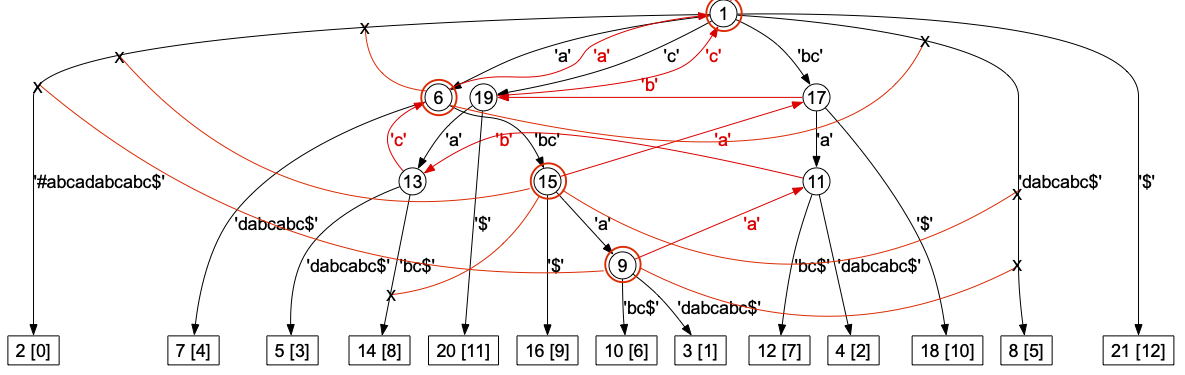
\includegraphics[width=1.00\textwidth]{fig/exp1/fwdstree_org.png}
%% \smallskip
%% \caption{
%%   Illustration of search strategies for maximal repeat enumeration on a string
%%   $S = \mathtt{\#abcadabcabc\$}$ of \cref{tbl:arrays}. 
%%   %S=#abcadabcabc$.
%%   The figure shows the suffix tree (black) and Winer tree (red) of $S$, highlighting maximal repeats with red double circles. Nodes represent right-branching substrings labeled with its SA-range, and edges are labeled with strings (black) or characters (red). Previous methods $\BUSA$ and $\TDBW$ traverse entire subtrees, while our method $\MREnum$ efficiently traverses only relevant red nodes via black edges, significantly reducing the search space.
%% }\label{fig:fwdstree}
%% \end{figure}
%% %%%%%%


%% %%%%%%%%

%% \textbf{Previous work}.\ 
%% %%%%%
%% The current best upperbounds on the runtime of enumerating all distinct  maximal repeats were summarized as the following algorithm schema (see \cref{fig:fwdstree}).
%% The first scheme is abbreviated as \BUSA{} (bottom-up search with the suffix array),  and the best runtime was $O(n)$ time using $O(n)$ words of space based on $SA$, $ISA$, and the RMQ structure on $LCP$, shown by Narisawa, Inenaga, Bannai, and Takeda~\cite{narisawa2007efficient}. 
%% The second scheme is abbreviated as \TDBW{} (top-down search with the Burrows-Wheeler Transformation/BWT), and the runtime was $O(n \log\sigma)$ time using $O(n/\log_\sigma n)$ words of space based on the Wavelet tree on $BWT$, shown by Beller, Berger, and Ohlebusch~\cite{beller:berger2012space:efficient:bbo}.
%% %%where $ISA$ is the inverse $SA$, and $LCP$ is the longest common prefix array of the string.
%% After these seminal work with \textit{uncompressed indexes}~\cite{narisawa2007efficient,beller:berger2012space:efficient:bbo}, there have been a few recent researches on repetition-aware enumeration of maximal repeats with \textit{compressed indexes}~\cite{belazzougui2020linear,nishimoto:cpm2021enum}. For example, Nishimoto and Tabei~\cite{nishimoto:cpm2021enum} have nicely reduced the space to $O(r(S))$ with polylogarithmic factor retaining $O(n)$ time based on a variant of the \textit{$r$-index}. However, to the best of our knowledge, there have been no results that simutaneously achieve sublinear space and time sensitive to repetition parameters including $r(S), z(S)$, or $e_R(S)$. 


%% %%%%%%% tblnew.tex
%% %%% tabnew.tex
%% %\centering
%% \begin{table}[t]
%%   \caption{%
%%     Summary of the time and space of the previous and proposed algorithms for enumeration of all distinct maximal repeats in a string $S$ of length $n$,
%%     %of maximal repeats,
%%     %% where $\sigma$ is the alphabet size,
%%     %% $r$ is the number of BWT runs,
%%     %% $e_R$ is the number of right-extensions,
%%     %% %of maximal repeats,
%%     where
%%     $\sigma$, $r$, and $e_R$ are the numbers of 
%%     characters, BWT runs, and right-extensions, respectively, 
%%     $\delta$ is the substring complexity of $S$.
%%     See \cref{sec:prelim:ds:array} for abbreviations in column \textit{Data structure}, and BU/TD and SA/BW indicate bottom-up/top-down search and SA/BWT arrays, respectively, in \textit{Scheme}.
%% }\label{table:summary:new}
%% %%%% 
%% \medskip
%% \begin{minipage}{\textwidth}
%% %\hspace{-1.2em}
%% \begin{tabular}{%
%% p{.0em}%1margin
%% p{7.6em}%2algo
%% p{10.0em}%3underlying
%% >{\centering}p{7em}%5time
%% %>{\centering}p{8.5em}%6indexspace
%% >{\centering}p{8.5em}%%6indexspace
%% p{3.0em}%4type
%% %c%7dammy
%% %>{}p{4.9em}%7dammy
%% }\toprule
%%   & Algorithm
%%   & Data Structure	
%%   %% & Underlying\break Structure	
%% %% & Index Space
%% & Space (words)
%% & Enum.~Time 
%% & Scheme \\
%% %%%%
%% \midrule 
%% %% \multicolumn{6}{l}{Existing array-based algorithms} \\
%% & Narisawa~\cite{narisawa2007efficient}	&
%% \textsc{Sa,\,Isa,\,Txt,\,Lcp}\cite{manber:myers1993suffixarrays} & $O(n)$	& $O(n)$ & \BUSA{} 	 \\
%% %% & Narisawa~\cite{narisawa2007efficient}	& SA\cite{manber:myers1993suffixarrays} & $O(n)$	& $O(n)$ & \BUSA{} 	 \\
%% %% & Okanohara+~\cite{okanohara2009text}	& SA\cite{manber:myers1993suffixarrays}\&FM\cite{Ferragina05:FM} & $O(n)$& $O(n\log\sigma)$	 & \bufwd 	 \\
%% & Beller+~\cite{beller:berger2012space:efficient:bbo} 	&
%% \textsc{Bwt,\,Wt}~\cite{Ferragina05:FM}
%% & $O(n/\log_\sigma n)$ & $O(n\log\sigma)$	& \TDBW{} \\
%% & Belazzougui+\cite{belazzougui2015space:unusual} 	&
%% \textsc{Bwt,\,Rdq}~\cite{belazzougui2020linear}
%% & $O(n/\log_\sigma n)$ & $O(n)$	& \TDBW{} 	 \\
%% %% & Belazzougui+\cite{belazzougui2020linear} 	& Belazzougui+\cite{belazzougui2020linear} & $O(n)$ & $O(n)$	& \TDBW{} 	 \\
%% %% & Belazzougui+\cite{belazzougui2020linear} 	& Belazzougui+\cite{belazzougui2020linear} & $O(n\log n\log\sigma)$ & $O(n)$	& \TDBW{} 	 \\
%% & Nishimoto+~\cite{nishimoto:cpm2021enum} 	& Gagie+~\cite{gagie:navarro:prezza2020fully} & $O(r\log({\frac n r})\log n)$ & $O(n\polylog n)$ & \TDBW{} 	 \\
%% %%%%%
%% %% \multicolumn{6}{l}{Proposed algorithms} \\
%% \\
%% & [This paper]	&
%% \makebox[11em][l]{\textsc{Sa,\,Isa,\,Txt,\,Rmq$_\textsc{LCP}$}\!\cite{manber:myers1993suffixarrays}}
%%  & $O(n)$ & $O(e_R)$	& \MREnum	 \\
%% %% & [This paper]	& SA\cite{manber:myers1993suffixarrays} & $O(n)$ & $O(e_R)$	& \MREnum	 \\
%% & [This paper]   	& Gagie+~\cite{gagie:navarro:prezza2020fully}	 	& $O(r\log({\frac n r})\log n)$ & $O(e_R \log({\frac n r}))$& \MREnum \\
%% & [This paper]   	& $\delta$-SA~\cite{kempa:kociumaka2023collapsing}  & $O(\delta\log({\frac n \delta}) \log n)$	& $O(e_R \log^{4+\eps}(n))$	 & \MREnum  \\
%% \bottomrule
%% \end{tabular}
%% \end{minipage}
%% \end{table}
%% %%%%%%%

%% %% In particular, we are interested in the complexity of enumerating maximal repeats for highly-repetitive strings, in terms of repetition measures, which take smaler values than the length $n$ of a string. For instance, collections of human genome sequences with small pertabations and Wikipedia documents with edit history are examples of highly-repetitive strings. In highly repetitive strings, a number of measures of repetition growing sublinearly in the length of the string. Particularly, we focus on the repetition measure $e_R(S)$ associated to maximal repeats, introduced by Belazzougui \textit{et al.}~\cite{belazzougui:cunial:gagie:prezza:raffinot2015composite} in 2015, where $e_R(S)$ is the number of right-extensions of maximal repeats in a string~$S$. It is shown by~\cite{belazzougui:cunial:gagie:prezza:raffinot2015composite} that the measure $e_R$ is lowerbounded by other well-known repetition measures $r(S)$ and $z(S)$, the number of runs in the BWT and the number of LZ-phrases of $S$, respectively. 

%% %In this paper, we prove the following theorem.
%% %% To overcome this problem, we propose a simple and faster algorithm with a novel search strategy, which has not been examined so far by the previous work~\cite{narisawa2007efficient,beller:berger2012space:efficient:bbo,belazzougui2020linear,nishimoto:cpm2021enum}.  
%% %% We prove the following theorem.
%% %% To overcome this problem, we propose a simple and faster algorithm scheme, abbreviated \MREnum (top-down search with the suffix array), with a novel search strategy, which has not been examined so far by the previous work~\cite{narisawa2007efficient,beller:berger2012space:efficient:bbo,belazzougui2020linear,nishimoto:cpm2021enum}.  

%% \textbf{Goal of research and main results}.\ 
%% %%%%%
%% To overcome this problem, we propose a novel search scheme, abbreviated as \MREnum{} (top-down search with the suffix array), suitable for simple and faster algorithms, which has not been examined so far by the previous work~\cite{narisawa2007efficient,beller:berger2012space:efficient:bbo,belazzougui2020linear,nishimoto:cpm2021enum}.  
%% We prove the following theorem.

%% %% \begin{trivlist}\item[] \textbf{\cref{thm:algo:main}}
%% %%   Let $S$ be a string of length $n$ over an alphabet of $\sigma\ge 2$ symbols.  We assume any data structure that stores $S$ in $s_\fn{acc}(n)$ words of space supporting (i) access to $SA[i]$ and $ISA[i]$, and (ii) $RMQ_{LCP}(L, R)$ on $LCP$ in $t_\fn{acc}(n)$ worst-case time.
%% %% Then, all of distinct maximal repeats in $S$ can be enumerated in $O(e_R\cdot t_\fn{acc}(n))$ time and $O(\sigma^2 \log e_R)$ words of working space, where $\mu$ is the number of distinct maximal repeats in $S$ and  $e_R$ is the number of the right-extensions of maximal repeats such that $\mu \le e_R \le n$. 
%% %% \end{trivlist}

%% \begin{theorem}[main result]\label{thm:algo:main}
%%   Let $S$ be a string of length $n$ over an alphabet of $\sigma\ge 2$ symbols.
%%   We assume any data structure that stores $S$ in $s_\fn{acc}(n)$ words of space supporting (i) access to $SA[i], ISA[i]$, and $S[i]$, and (ii) $RMQ_{LCP}(L, R)$ on $LCP$ in $t_\fn{acc}(n)$ worst-case time.
%% Then, all of distinct maximal repeats in $S$ can be enumerated in $O(e_R\cdot t_\fn{acc}(n))$ time and $O(\sigma^2 \log e_R)$ words of working space, where $\mu$ is the number of distinct maximal repeats in $S$ and  $e_R$ is the number of their right-extensions such that $\mu \le e_R \le n$. 
%% \end{theorem}

%% By substituting different SA index for \cref{thm:algo:main} above, we obtain a variety of enumeration algorithms for distinct maximal repeats with different time and space trade-offs.
%% In \cref{table:summary:new}, we show the summary of results. 
%% %% 
%% Firstly, we observe the case with the uncompressed SA index of Manber and Myers~\cite{manber:myers1993suffixarrays}, and the RMQ structure $RMQ_{LCP}$ on $LCP$ by Bender and Colton~\cite{bender:colton2000thelcaproblem}. 

%% \begin{theorem}\label{thm:algo:uncompressed:sa}
%%   All distinct maximal repeats in a string $S$ of length $n$ can be enumerated in $O(e_R)$ time and $O(\sigma^2 \log n)$ working space based on $SA, ISA, S$, and $RMQ_{LCP}$ using $O(n)$ words of space. 
%% \end{theorem}

%% Secondly, we observe the cases with the repetition-aware, compressed SA indexes, namely,
%% the \textit{$r$-index} with $O(r\polylog(n))$ space by Gagie \textit{et al.}~\cite{gagie:navarro:prezza2020fully}, and
%% the \textit{$\delta$-spaced SA index} with $O(\delta\polylog(n))$ space by Kempa and Kociumaka~\cite{kempa:kociumaka2023collapsing}, where $\delta \le r \le e_R$ (see \cite{kociumaka:navarro:olivares2024near:delta:optimal,kempa2018roots,belazzougui:cunial:gagie:prezza:raffinot2015composite}).
%% Then, we obtain enumeration algorithms with $O(e_R\polylog(n))$ runtime and space simultaneously shown in the last two lines of \cref{table:summary:new} (\cref{thm:applications}, \ref{item:result:bidirect:index}--\ref{item:result:compressed:delta:index}). 
%% If $e_R = o(n/\log^c n)$ for $c\ge 1$ and $c\ge 4+\eps$, respectively, for hightly-repetitive strings (e.g., Fibonacci or Thue-Morse words~\cite{radoszewski:rytter2012structure:cdawg:thuemorse}), these results yield the first sublinear time and space MR enumeration. 


%% \textbf{Contributions}.\ 
%% %%%%%
%% In this paper, we presented a simple and modular algorithm for enumerating all distinct maximal repeats by using $SA$ and associated auxiliary structures as black box.
%% Technically, the key to our results with time and space complexities that are  sensitive to the repetitiveness measure $e_R$ is a simple and modular algorithm with a novel search strategy (see \cref{fig:fwdstree}), which has not been used before for this problem. 
%% Overall, this work presents the first sublinear, repetitiveness-aware algorithms for highly repetitive strings.

%% %% To overcome the difficulties of the previous approaches, we propose a simple and faster algorithm with a novel search strategy, which has not been examined so far by the previous work~\cite{narisawa2007efficient,beller:berger2012space:efficient:bbo,belazzougui2020linear,nishimoto:cpm2021enum}

%% %% \begin{toappendix}
%% %% We discuss the following applications. 
%% %% In addition to maximal repeats, much attention has been paid to other string patterns in bioinformatics such as minimal absent words (MAWs)~\cite{barton2014linear}, minimal unique substrings (MUSs)~\cite{ilie2011minimum}, and their generalization called minimal rare words (MRWs)~\cite{belazzougui2015space:unusual}. We also focus on these string patterns because they are closely related to maximal repeats~\cite{inenaga2024computing}.
%% %% For applications, our algorithm significantly improves the running times of the previous $O(n)$-time algorithms~\cite{barton2014linear,ilie2011minimum,belazzougui2015space:unusual} based on the suffix array $SA$ with auxiliary structures, for sequence patterns including MAWs, MUSs, and MRWs related to maximal repeats. We also discuss application of our algorithm to faster construction of the CDAWG string index with $SA$. 
%% %% \end{toappendix}

\textbf{Organization of this paper}.\ 
%%%%%
\cref{sec:prelim} introduces basic notions and definitions, necessary to the rest of this paper. 
%% \cref{sec:prev} gives a brief review on the previous approaches in maximal repeats enumeration.
In \cref{sec:mrep} and \cref{sec:algo}, we first present a basic algorithm for enumerating the set $\MR(S)$ of all of $occ$ maximal repeats of a string $S$ over alphabet $\Sigma$ can be enumerated in $O(e_R + occ)$ time and $O(e_L  + |\Sigma|^2 \log n)$ working space, where $n$ is the length of $S$. 
In \cref{sec:mrw}, we extend the basic algorithm to afoementioned classes of unusual words, and show that the set of all patterns of a string $S$ within any of these classes can be enumerated in $O(e_L + e_R + occ)$ time, and give its correctness and computational complexity.
In \cref{sec:conc}, we conclude. 


\input{review}
%% algo.tex
%% \section{The Proposed Algorithm}
\section{A Simple and Faster Algorithm}
\label{sec:algo}
%%%% 
Now, we present our $O(e_R)$-time algorithm scheme $\TDSA$ (\textit{top-down search with the suffix array}) for enumerating all distinct maximal repeats of a string $S$,  based on $SA$, $ISA$, $S$, and the RMQ structure on $LCP$ of a text $S$ using $O(n)$ words of space, where $e_R \le n$ is the measure of repetitiveness of a text, namely, the number of right-extensions.


%%%%%%%%%%%%%%%%%
{
  \setlength{\interspacetitleruled}{0pt}%
  \setlength{\algotitleheightrule}{0pt}%  
  \begin{algorithm}[h]
  %% \caption{Top-down MR-enumeration algorithm with SA}\label{algo:maxrep:tdfw}
  \textbf{Procedure} \TDSA$(\tau_0 = ([L_0..R_0], \ell_0))$:\\
  %%\KwGiven{}
  %% \KwIn{The triple $\tau_0 = (L_0, R_0, \ell_0)$ for a right-branching substring $X$ of a text.}
  %% \KwOut{}
  \Begin{
      \textbf{output} $\tau_0$
      \Comment*{A maximal repeat is found}
      \For %(\CM{})
           {child $\tau = ([L..R], \ell)$ of the parent $([L_0..R_0], \ell_0)$}{
          \Comment{It is ensured that $R - L \ge 1$ and $\tau$ is right-branching}
          Decide if $\tau$ is left-branching by $SA, ISA$, and $S$ (\cref{lem:leftmaximal:character})\; 
          \If {$\tau$ is left-branching}{          
            \TDSA$(\tau)$\; 
          }
        }
  }
  \end{algorithm}
}  
%%%%%%%%%%%%%%%%%

\subsection{Search strategy}
\label{sec:algo:tdsa}
%%%% 
A basic idea of $\TDSA$ is the use of \textit{top-down search} using the forward search for right-extensions based on the \textit{suffix array}, unlike the backward search for right-extensions adopted by \TDBW.
This enables the sound and early pruning of hopeless right-extensions that never become left-branching ones.
%% 
Now, we define the parent-child relation over triples related to the suffix tree of $S$ as follows. For triples $\tau_0 = ([L_0..R_0], \ell_0)$ and $\tau = ([L..R], \ell)$ defining strings $U$ and $W$, $\tau$ is called the \textit{$b$-child} of $\tau_0$ if $W = Ub$ for some character $b \in \Sigma$, called a \textit{branching character}. The ancestors and descendants of $\tau$ are defined in the standard manner.
%%We have. 

\begin{lemma}\label{lem:prune:leftbranch}
Suppose that a triple $\pi$ is an ancestor of a triple $\tau$. If the substring defined by $\tau$ is left-branching, the substring defined by $\tau$ is also left-branching. 
\end{lemma}

Recall that a repeat is maximal if and only if it is both left- and right-maximal in $S$. Lemma~\cref{lem:prune:leftbranch} says that the set $MR(S)$ occupies the \textit{upper connected region} of the suffix tree of $S$. For instance, we see in \cref{fig:fwdstree} that $MR(S)$ occupies the node sets $\set{1,6,15,9}$. 
%% In other words, if a triple $\tau$ is not left-branching, then any of its ancestor is also not left-branching.
This implies the next rule.

\begin{itemize}\item[]
\quad\textsc{Pruning rule}: {Every non-left-branching triple is pruned.}
\end{itemize}

For testing the left-branching property, we use the following lemma, which is a slight modification of Narisawa \textit{et al.}~\cite[Lemma~10]{narisawa2007efficient}. 

%% \begin{lemma}\label{lem:leftmaximal:character}
%% Let $W$ be any substring of $S$ and $\tau = (L,R, \ell)$ be the triple defining~$W$. 
%% Then,
%% %% the following conditions (1)--(3) are equivalent each other: 
%% (1) $W$ is not left-branching in $S$ if and only if  
%% (2) $(R - L + 1) = (ISA[SA[L]-1] - ISA[SA[R]-1] + 1)$. 
%% \end{lemma}

\begin{lemma}[Narisawa \textit{et al.}~\cite{narisawa2007efficient}]\label{lem:leftmaximal:character}
For the triple $\tau = (L,R, \ell)$ for any substring~$W$ of $S$, 
(1) $W$ is not left-branching in $S$ if and only if  
(2) (i) $S[p-1] = S[q-1]$ and (ii) $R - L = \id{ISA}[p-1] - \id{ISA}[q-1]$ with $p = SA[L]$ and $q = SA[R]$.
\end{lemma}

\begin{proof}
%%We add clause (*)  
We let $p = SA[L], q = SA[R]$. 
$(1)\Implies (2)$: Suppose that $W$ is not left-branching in $S$.
Then, all occurrences of $W$ in $S$ have the same previous characters $c \in \Sigma$ in $\spos(W)$. Thus, it immediately follows that $BWT[L, R]$ is monotone.
Let $\varphi: k \mapsto ISA[SA[k]-1]$. By observing $\varphi$ coincodes to the LF-mapping~\cite{Ferragina05:FM}, claim (2) immediately follows. 
%%% 
$(2) \Implies (1)$: 
%We show the contraposition $\neg (1) \Implies \neg (2)$. 
Suppose (2), and to contradict that $\neg$(2) $W$ is left-branching in $S$. Let $I = [L..R]$. Then, there exist a pair of preceding characters $c = S[p-1], d=S[q-1]$ with $c\not= d$ for some $p, q \in \spos(W)$. It follows that $\varphi$ transforms the positions in  $SA[L..R]$ into at least two, mutually disjoint, non-empty ranges $I_c, I_d$ with $I_c\uplus I_d = I$ starting with $c$ and $d$, respectively. By assumption (2.i), we see that positions $SA[L]$ and $SA[R]$ move into the same range, say $I_c$ with $L_c := \varphi(L)$ and $R_c := \varphi(R)$ as the left and right ends of $I_c$ since $\varphi$ preserves $<_\lex$. 
Since both of $I_c$ and $I_d$ are non-empty, we have $R_c - L_c + 1 = |I_c| < |I| = R - L + 1$; contradiction to assumption (2.ii). By contradiction, we conclude condition (1) holds. 
\qed   
\end{proof}

%% \begin{proof}
%% We add clause (*)  $BWT[L, R]$ is monotone. 
%% We let $p = SA[L], q = SA[R]$. 
%% $(1)\Implies (*)$: Suppose that $W$ is not left-branching in $S$. Then, we see that all occurrences of $W$ in $S$ have the same character, say $c$, in the previous positions in $\spos(W)$. Thus, the claim (*) immediately follows. 
%% %%% 
%% $(*) \Implies (2)$: We can easily observe that the function $f(k) := ISA[SA[k]]$ realizes the LF-mapping~\cite{Ferragina05:FM} by definition. Hence, claim (2) immediately follows from (*). 
%% %%% 
%% $(2) \Implies (1)$: 
%% %We show the contraposition $\neg (1) \Implies \neg (2)$. 
%% Suppose that $W$ is left-branching in $S$. Then, it follows that $c = S[p-1]\not= S[q-1] = d$ for some $p, q \in\spos(W)$ of $W$. 
%% %It follows that the subarray $BWT[L,R]$ contains mutually distinct $c$ and $d$. Since $[L,R]$ is the SA-interval of $W$, 
%% Therefore, the substring $W$ has a pair of distinct characters $c = S[p-1]$ and $d = S[q-1]$ at the previous positions of its start positions. By contraposition, $W$ is left-branching. 
%% Combining the above arguments, the lemma is proved. 
%% \qed   
%% \end{proof}

\subsection{Computing the set of child triples}
\label{sec:algo:branch}
%%%% 
%% An SA-range $[L..R]$ is called an $\ell$-range if it satisfies the conditions (i)--(iv) below: 
%% \begin{enumerate*}[(i)]
%% \item $LCP[L] < \ell$, 
%% \item $LCP[L] \ge \ell$ for all $k \in [L+1..R]$, 
%% \item $LCP[L] = \ell$ for at least $k \in [L+1..R]$, and 
%% \item $LCP[R+1] < \ell$.  
%% \end{enumerate*}
An SA-range $[L..R]$ is called an \textit{$\ell$-range} if the lcp of all suffixes starting  with positions in $SA[L..R]$ equals~$\ell$, i.e.,
$\ell = \min\sete{ SA[k] \mid k \in [L+1..R] }$. 
Then, an index $k \in [L+1..R]$ is called a \textit{$\ell$-index} if it achieves the lcp-value $\ell$, i.e., $LCP[k] = \ell$.
Cosider the suffix tree $\sig T$ of a string $S$.
%% We say that a triple $\tau = ([L..R], \ell)$ is a child of triple $\tau_0 = ([L_0..R_0], \ell_0)$ 
If triples $\tau_0$ and $\tau$ represent string labels of a node $u$ and its child $w$ in the suffix tree (see gusfield1997book:stree), we say that the range $[L..R]$ is a \textit{child} of the range $[[L_0..R_0]]$. 
%% 
For computing the set of child ranges of a given $\ell$-range $[L_0, R_0]$, we use the following lemma.

\begin{lemma}[Abouelhoda, Kurtz, and Ohlebusch~\cite{abouelhoda2004replacing}]\label{lem:child:ranges}
  Let $[L_0, R_0]$ be any $\ell$-range.
  If $M_1 < M_2 < \dots < M_k$ are the $\ell$-indexes in ascending order, then the child ranges of $[L_0, R_0]$ are
  $[L_0..M_1-1], 
   [M_1..M_2-1], 
   \ldots,
   [M_k..R_0]$.  
\end{lemma}

Although Abouelhoda \textit{et al.}~\cite{abouelhoda2004replacing} presented based on \cref{lem:child:ranges} how to use an array $\op{childtab}[1..n]$ of cells with three integer fields $\op{up}, \op{down}$, $\op{nextIndex} \in [n]$ for traversing the virtual suffix tree top-down, the method is not suitable to our purpose. 
%%% 
Instead, combining \cref{lem:child:ranges} above and the recursive procedure for colored range query by Muthukrishnan~\cite{muthukrishnan2002efficient} (see also the textbook by Ohlebusch~\cite{ohlebusch2013bookbioinfo}), we present a recusive procedure \proc{BranchRepeats} for enumerating the set of all child ranges of an $\ell$-range below, invoked in the top-level as \proc{BranchRepeats}$([L..R], \ell_*)$ with $\ell_* = RMQ_{LCP}(L+1, R)$. 

%%%%%%%%%%%%%%%%%
{
\setlength{\interspacetitleruled}{0pt}%
\setlength{\algotitleheightrule}{0pt}%  
\begin{algorithm}[h]
  \textbf{Procedure} \proc{BranchRepeats}$([L..R], \ell_*)$:\\  
  \Begin{
      \If {$R - L \ge 1$}
      {
        $(M, \ell) \gets RMQ_{LCP}(L+1, R)$
        \Comment*{$\ell = LCP[M]$}
        \iIf {$\ell_* < \ell$}{
          \textbf{output} $(L, R, \ell)$
          \Comment*{$[L,R]$ is monotone}
        }
        \Else  (\CM{$\ell_* = \ell$} and $[L,R]$ is diverse) 
        {
          $\proc{BranchRepeats}([L..M-1], \ell_*)$\; 
          $\proc{BranchRepeats}([M..R], \ell_*)$\;
        }
      }
  }
\end{algorithm}
}
%%%%%%%%%%%%%%%%%

By using the RMQ structure on $LCP$ that supports constant time queries, the procedure correctly computes the answers in output-sensitive manner. 


\begin{lemma}[Muthukrishnan~\cite{muthukrishnan2002efficient}, Ohlebusch~\cite{ohlebusch2013bookbioinfo}]
  The set of all child ranges of an $\ell$-range $[L..R]$ can be enumerated in $O(k)$ time in $O(n)$ space
  using $RMQ_{LCP}$, 
%% using the RMQ structure on $LCP$, 
where $k$ is the number of the child renges to output.  
\end{lemma}


%%%%%%%%%%%%
\subsection{Execution example}

In \cref{fig:run:example}, we show an example run of Algorithm $\TDSA$ for a text $S[0..10] = \mathtt{\#aabaababb\$}$. The black and red trees, respectively, indicate the suffix and the Weiner trees of $S$. Each circle indicates a node with the string label and the triple. A gray node corresponds a maximal repeat. 
We observe that the proposed algorithm $\TDSA$ only traverses the suffix tree starting from the root, and enumerates all maximal repeats, by visiting all and only the gray nodes. 


%%%%%%%%%%%%
\subsection{Complexity Analysis}
%%%%%
As the main result, we show \cref{thm:algo:main}, 
combining Lemmas~\ref{lem:prune:leftbranch},
\ref{lem:leftmaximal:character}, and 
\ref{lem:child:ranges}.
%% \cref{lem:prune:leftbranch},
%% \cref{lem:leftmaximal:character}, and 
%% \cref{lem:child:ranges}.

%% \begin{trivlist}\item[]
%% (\textit{The proof for \cref{thm:algo:main}})\quad   
%% \begin{proof}
\begin{statement}{The proof for \cref{thm:algo:main}}
  From \cref{lem:prune:leftbranch}, we observe that any maximal repeat (MR) $W \in MR(S)$ is either (i) the empty string $\eps \in MR(S)$, where $|\Sigma|\ge 2$, or (ii) there exists a shorter MR $U \in MR(S)$ and a $b \in \Sigma$ exactly when (ii.a) $W = \rext{Ub}$ and (ii.b) $\lext{W} = W$.
  By \cref{lem:child:ranges}, we can obtain such a $b \in \Sigma$ in (ii.a), and by \cref{lem:leftmaximal:character}, we can make test in (ii.b) in $O(1)$ time. 
  Combining the above arguments, the correctness and time complexities follows. 
  %%% 
  To bound the working space, we use the technique by Belazzougui \textit{et al.}~\cite[Lemma~4.2]{belazzougui2020linear} as follows. Consider the suffix tree $\sig T$ of $S$ as the search tree of our algorithm. At each iteration in the top-down traversal, we first select the child with the widest SA-range, having the largest number of leaves. Since this generetes the heavy-leaf decomposition of $\sig T$, the modified traversal yields at most $O(\log n)$ levels with $O(\sigma^2)$ side information per level, each has $O(1)$ size in $\sig T$. This leads to the working space of $O(\min\set{e_R, \sigma\log n}) = O(\sigma^2\log n)$ words. \qed 
\end{statement}

%%%%%%
\begin{figure}[t]
  \centering
  \rule{0.09\textwidth}{0em}
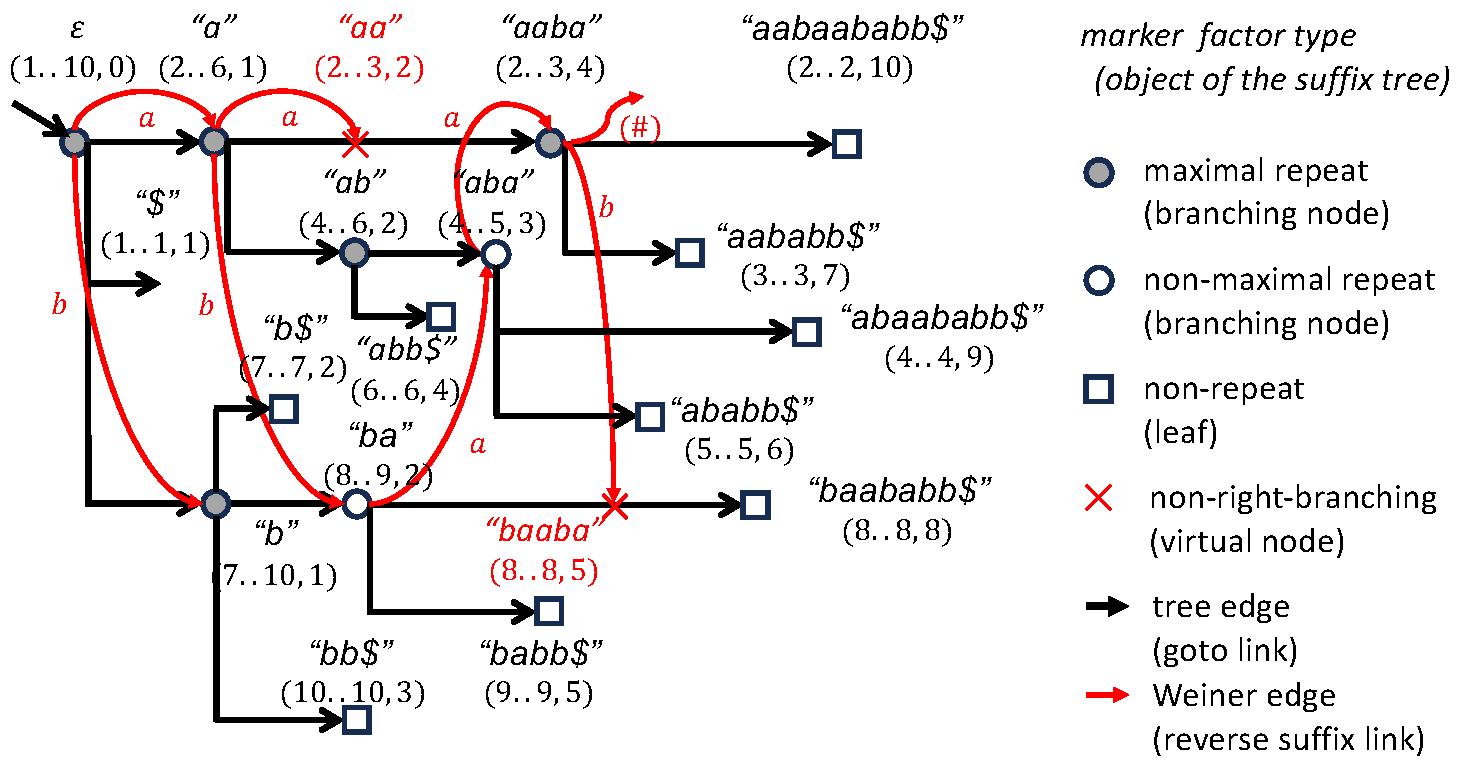
\includegraphics[width=0.9\textwidth]{fig2.pdf}
\vspace{.75\baselineskip}
\caption{An example run of Algorithm $\TDSA$ for a text $S = \mathtt{aabaababb\$}$, where the left endmarker $S[0]=\#$ and the related suffixes are omitted. 
}\label{fig:run:example}
\end{figure}
%%%%%%

%% %%%%
%% \subsection{Time-space trade-offs }
%% \label{sec:appl}

For the uncompressed SA index, the next result follows. 

\begin{statement}{The proof for \cref{thm:algo:uncompressed:sa}}
  From \cref{thm:algo:main} above, we obtain the next result by subsitution $t_\fn{acc}(n) = O(1)$ time and $s_\fn{acc}(n) = O(n)$ words from Manber and Myers~\cite{manber:myers1993suffixarrays}.
  \qed 
\end{statement}

%% \begin{trivlist}\item[] \textbf{\cref{thm:algo:uncompressed:sa}}
%%   All distinct maximal repeats in a string $S$ of length $n$ can be enumerated in $O(e_R)$ time and $O(\sigma^2 \log n)$ working space using $O(n)$ space based on $SA$, $ISA$, and the RMQ structure on $LCP$.
%% \end{trivlist}

%% \begin{theorem}\label{thm:algo:uncompressed:sa}
%%   All distinct maximal repeats in a string $S$ of length $n$ can be enumerated in $O(e_R)$ time and $O(\sigma^2 \log n)$ working space using $O(n)$ space based on $SA$, $ISA$, and the RMQ structure on $LCP$.
%% \end{theorem}


\begin{toappendix}
In \cref{table:arrays:hybrid}, we show the list of underlying data structures, implementing the indexing arrays in \cref{sec:prelim:ds:array}, used in \cref{sec:prev} and \cref{sec:algo}. 
%%%%%%%%%%
%%% table2.tex : basic text indexing structures
%%%%% table2.tex

%% basic text indexing structures : array-based 
\begin{table}[t]\centering\tabcolsep=.25em
\caption{Array-based text indexing structures for static texts, where
the columns SA, ISA, TA, and LCE indicate the times for accessing the  suffix and the inverse suffix arrays, text $T$, and the LCE query. See \cref{table:summary} for $s_r(n)$  and $s_\delta(n)$. 
}\label{table:arrays}
\medskip
\begin{tabular}{l>{\centering}p{5em}>{\centering}p{7em}cccclll}\toprule
Structure	& Construct\-ion time   & Space (words) & \multicolumn{3}{c}{Query time}	\\
\cmidrule{4-6}
& &  & SA \& ISA	& TA	& LCE	 \\
  \midrule
MM~\cite{manber:myers1993suffixarrays}	& $O(n)$   & $O(n)$	& $O(1)$	& $O(1)$	& $O(1)$	\\
Belazzougui+~\cite{belazzougui2020linear} & $O(n)$   & $O(n\log n/\log\sigma)$	& $O(1)$	& $O(1)$	& $O(1)$	\\
%$s_r(n) = O(r\log(n/r)\log n)$, 
Gagie+~\cite{gagie:navarro:prezza2020fully}	& $s_r(n)$   & $O(r\log(n/r))$	& $O(\log(n/r))$	& $O(\log(n/r))$	& $O(\log(n/r))$	\\
Kempa+~\cite{kempa:kociumaka2023collapsing}	& $s_\delta(n)$   & $O(\delta \log\frac{n\log\sigma}{\delta\log n})$	& $O(\log^{4+\eps} n)$	& $O(\log n)$	& $O(\log n)$	\\
%% na	& sp	& sa	& isa	& ta	& lce	& reference \\
\bottomrule
\end{tabular}
\end{table}
%% EOF


 %% static indexes 
%% basic text indexing structures : array-based 
\begin{table}[h]\centering\tabcolsep=.25em
\caption{%%
  Array-based text indexing structures, where SA, ISA, Txt, and RMQ$_\fn{LCP}$ indicate the access and query time to the respective structures.
}\label{table:arrays:hybrid}
\medskip
\begin{tabular}{l>{\centering}p{7em}>{\centering}p{4em}cccclll}\toprule
  Structure  & Space & Constr. & \multicolumn{3}{c}{Query time}	\\
\cmidrule{4-6}
& (words) & time  & SA \& ISA	& Txt	& RMQ$_\fn{LCP}$
\\
  \midrule
Manber+~\cite{manber:myers1993suffixarrays}	& $O(n)$   & $O(n)$	& $O(1)$	& $O(1)$	& $O(1)$	\\
Ferragina+~\cite{Ferragina05:FM}  & $O(n\log n/\log\sigma)$	& $O(n)$  & $O(1)$	& ---	& ($O(1)$ WT)	\\
%$s_r(n) = O(r\log(n/r)\log n)$, 
%% Belazzougui+~\cite{belazzougui2020linear}  & $O(n\log n/\log\sigma)$	& $O(n)$  & $O(1)$	& $O(1)$	& $O(1)$	\\
%% %$s_r(n) = O(r\log(n/r)\log n)$, 
Gagie+~\cite{gagie:navarro:prezza2020fully}	& $O(r\log(n/r))$	& See~\cite{gagie:navarro:prezza2020fully}   & $O(\log(n/r))$	& $O(\log(n/r))$	& $O(\log(n/r))$	\\
Kempa+~\cite{kempa:kociumaka2023collapsing}	& $O(\delta \log\frac{n\log\sigma}{\delta\log n})$	& See~\cite{kempa:kociumaka2023collapsing}   & $O(\log^{4+\eps} n)$	& $O(\log n)$	& $O(\log n)$	\\
%% na	& sp	& sa	& isa	& ta	& lce	& reference \\
\bottomrule
\end{tabular}
\end{table}
%%%%%%%%%%
\end{toappendix}

%%% 
Next, we present the following results on the time-space trade-offs of our algorithm $\TDSA$ in \cref{thm:algo:main} by varying an underlying SA-index structure supporting $SA$, $ISA$, and $RMQ_{LCP}$.

%%\cref{thm:applications}\cref{item:result:compressed:r:index}    

\begin{theoremrep}[Time-space trade-off]\label{thm:applications}
  We can enumerate the set $MR(S)$
  %of all distinct maximal repeats
  in a string $S$ of length $n$ over an alphabet of $\sigma\ge 2$ symbols in the following time and space complexities, where the working space is always $O(\sigma^2 \log e_R)$. 
  %%%% 
\newcommand{\mylistheading}{\textbf}
  \begin{enumerate}[(a)]

\item \mylistheading{Bi-directional SA-index}:    
  The set $MR(S)$ can be enumerated in $O(\min\set{e_L, e_R})$ time and $O(n)$ space using the uncompressed SA-indexes for $S$ and $S\rev$. 
  \label{item:result:bidirect:index}
    
  \item \mylistheading{$r$-sized SA-index}:
    The set $MR(S)$  can be enumerated in $O(e_R \log {\frac n r})$ time and $O(r\log {\frac n r}\log n)$ space using the $r$-index by
    Gagie et al.~\cite{gagie:navarro:prezza2020fully}.
      \label{item:result:compressed:r:index}    
    %% Gagie et al., Navarro, and Prezza~\cite{gagie:navarro:prezza2020fully}.
    %%   \label{item:result:compressed:r:index}    
    
  \item \mylistheading{$\delta$-sized SA-index}:
    The set $MR(S)$ can be enumerated in $O(e_R \log^{4+\eps}(n))$ time and $O(\delta\log({\frac n \delta}) \log n)$ space using the compressed SA with $\delta$-space, proposed by Kempa and Kociumaka~\cite{kempa:kociumaka2023collapsing}.
          \label{item:result:compressed:delta:index}
  \end{enumerate}
\end{theoremrep}

\begin{proof}
By substituting the data structures in \cref{table:arrays:hybrid} for the algorithm scheme $\TDSA$, the results immediately follows from \cref{thm:algo:main}. \qed
\end{proof}

Related to \ref{item:result:bidirect:index} of \cref{thm:applications}, Inenaga and Kosolobov~\cite{inenaga:kosolobov2024relating:left:right} recently showed that $e_R(S)$ and $e_L(S)= e_R(S\rev)$ are polynomially related with factor $\Theta(\sqrt{n})$. 
%%$\max\set{e_R(S)/e_L(S), e_L(S)/e_R(S)} = O(\sqrt{n})$. 


   %%  In this paper, we studied the problem of enumerating all distinct maximal repeats in a given string using the suffix array (SA) in relation to a repetitiveness measure $e_R$ of the number of right-extensions in a string. After examining the previous approaches, we presented a simple and efficient algorithm with novel search strategy. We proved that the proposed algorithm runs in $O(e_R)$ time based on the SA, inverse SA, and the range-minima query on the LCP array. We also show that
   %% all maximal repeats can be enumerated in $O(e_R \;\textrm{polylog}(n))$ time and space simultaneously using existing compressed text indexes. 
   %%  This is the first result on the repetitiveness-aware sublinear time algorithm for highly-repetitive strings. 


%% %%%%%%%%%%%%%%%%%
%% \begin{algorithm}[h]
%%   \caption{Enumerating all distinct maximal repeats in a string}\label{algo:maxrep:tdfw}
%%   \stringbf{Procedure} \stringsc{MaxRepTD}$(\tau = (L_0, R_0, \ell_0))$:\\
%%   %%\KwGiven{}
%%   \KwIn{The triple $\tau_0 = (L_0, R_0, \ell_0)$ for a right-branching substring $X$ of a string.}
%%   %% \KwOut{}
%%   \Begin{
%%       \stringbf{output} $\tau$
%%       \Comment*{A maximal repeat is found}
%%       %% $C \gets \emptyset$\; 
%%       %% $\stringsc{BranchRepeats}(\tau_0, C)$\; 
%%         \For (\CM{$R - L \ge 1$ must hold}) {$(L, R)\in \stringsc{BranchRepeats}(\tau_0)$}{
%%         %% \For (\CM{$R - L \ge 1$ must hold}) {$(L, R)\in C$}{
%%           $\tau \gets (L, R, \ell)$ with $\ell \gets RMQ_{LCP}(L+1, R)$
%%           \Comment*{$\tau$ is right-branching}
%%           Decide if $\tau$ is left-branching by SA and ISA (\cref{lem:leftmaximal:character})\; 
%%           \If {$\tau$ is left-branching}{          
%%             \stringsc{MaxRepTD}$(\tau)$\; 
%%           }
%%         }
%%   }
%% \end{algorithm}
%% %%%%%%%%%%%%%%%%%

%%new
%%%% algo.text


%%%%%%%%%%%%%%%%
\section{Algorithm~A: The Proposed Algorithm with Suffix Array}
%% \section{The Proposed Algorithm}
\label{sec:algo:forward}

In this section, we present the first algorithm that enumerates all maximal repeats in a text $T$ of length $n$ in $O(e_R)$ time
%and $O(\sigma^2 \log e_\fn{min})$ words of working space
using precomputed arrays, namely, the suffix, inverse suffix, and LCP arrays, namely $SA[1,n], ISA[1,n]$, and $LCP[1,n]$, occupying $O(n)$ words space. It traverses the DFS over the virtual suffix tree for $T$ using the above arrays. 

In what follows, we assume any data structure for storing $SA[1,n], ISA[1,n]$, and $LCP[1,n]$, where $LCP$ is equipped with $RMQ$~\cite{bender:colton2000thelcaproblem}, using $s(n)$ words of space, after $p(n)$ preprocessing of $T$, supporting 
access to the arrays in $t_\fn{acc}(n)$ time in the worst-case. 


%%%%%%%%%%%%%%%%%
\begin{algorithm}[t]
  \caption{The algorithm for enumerating the rich representations of all maximal repeats in an input text $T[1,n]$ of length $n$ in $O(e_R)$ time by traversing the virtual suffix tree for $T$ using the suffix, inverse suffix, and longest common prefix arrays, $SA, ISA$, and $LCP$ of~$T$. In the top-level, the procedure is invoked with the rich representation $(1, n, 0)$ with the empty string $\eps$. 
  }\label{algo:maxrep:fwd}
  \textbf{Procedure} \textsc{MaxRepeatsSA}$(L, R, \ell)$:\\
  \KwIn{A rich-representation $(L, R, \ell)$ consisting of an SA-interval $[L, R]$ and an $\ell\ge 0$ for a right-branching substring $U$ of $T$}
  %% \KwOut{}
  \Begin{
      \textbf{output} $(L, R, \ell)$
      \Comment*{$(L, R, \ell) = repr(U)$}
      $\ell_* \gets \LCE(SA[L], SA[R])$\; 
      %%$\ell_* \gets \lcpmin(L, R)$\;       
        \For{$(L_c, R_c, \ell_c, c)\in \textsc{FRD}(L, R, \ell_*)$}{
          %\Comment{Notes: $\exists c \in \Sigma, \forall k \in [L',R'], T[SA[k]+\ell_*] = c$}
          $\ell' \gets \LCE(SA[L_c], SA[R_c])$
          %%$\ell' \gets \lcpmin(L_c, R_c)$          
          \Comment*{$(L_c, R_c, \ell_c) = repr(\rext{(Uc)})$}
          \uIf{$|[L_c, R_c]| = 1$}{
            continue; \Comment{Skip $(L_c, R_c, \ell_c, c)$}
          }
          \uElseIf (\Commentblock{\cref{lem:leftmaximal:character}}) {$(L_c, R_c, \ell_c)$ is left-branching }{          
            \textsc{MaxRepeatsSA}$(L_c, R_c, \ell_c)$\; 
          }
          \Else{
            \Comment{Pruning descendants of non-left maximal substrings}
          }
        }
  }
\end{algorithm}
%%%%%%%%%%%%%%%%%

\subsection{Outline of the Algorithm}
%%%%%
In Algorithm~\ref{algo:maxrep:fwd}, we show the main algorithm for enumerating all maximal repeats in a text. 
The key idea of our algorithm is to combine the virtual \textit{top-down traversal} of the suffix tree of $T$ with the suffix and LCP arrays of $T$, proposed by Abouelhoda, Kurtz, and Ohlebusch~\cite{abouelhoda2004replacing}, and the $O(1)$-time left-branchingity test by Narisawa \textit{et al.}~\cite{narisawa2007efficient}.

% We remark that this combination is new since (1) neither of the algorithms did not use the characterization of the existence of maximal repeats in the suffix tree that we will show below at all, and (2) Narisawa \textit{et al.}'s algorithm~\cite{narisawa2007efficient} was based on the \textit{bottom-up traversal} of the suffix tree with the suffix and LCP arrays, proposed by Kasai \textit{et al.}~\cite{kasai2001linear}.

First, we review the suffix tree of a text $T$~\cite{gusfield1997algorithms} in our terminology.
Formally, the suffix tree for $T$ is defined as follows. 

\begin{definition}[suffix tree]\rm
  \label{def:stree}
  For any text $T$, the suffix tree of $T$, denoted by $\stree(T)$, is an edge-labeled tree $C = (V, E)$ such that
  \begin{align*}
    V &= \sete{ \rext{U} \mid U \in \substr(T) },  
    \\
    E &=
    \sete{     (\rext U, a\beta, \rext{Ua})
      \mid \rext{U}, \rext{Ua} \in V, a\in\Sigma, \beta \in \Sigma^*,
      \rext{Ua} = U a\beta 
    }
    % \\
    % E &=
    % \sete{     (\rext U, \beta, U\beta)
    %   \mid U, U\beta \in V, a\in\Sigma, \beta \in \Sigma^+,
    %   \rext{Ua} = U\beta 
    % }
    \\
    F &=
    \sete{ (a\rext{U}, a, \rext{U})
      \mid a\rext{U}, \rext{U} \in V, a\in\Sigma
    }
  \end{align*}
where $\rext\eps \in V$ is the root. Elements of $E$ and $F$ are called \textit{foward edges} (or \textit{goto edges}) and \textit{suffix links}. 
\end{definition}

We let $W = F^{-1}$ to be the set of the inverse links of $F$, where its elements are called \textit{Weiner edges}, and call the edge-labeled tree $(V, W)$ the \textit{Weiner tree} (or the \textit{suffix link tree}) of $T$. 
In \cref{fig:fwdstree}, we show an example of the suffix tree $\stree(T)$ for a text $T = \mathtt{\#abcadabcabc\$}$ of length $n = 13$. In the figure, the circle and boxes indicate the branching nodes and leaves in $V$, respectively. Besides this, black and red arcs indicate the forward and backward edges in~ $E$, respectively. 

By \cref{def:stree}, we observe the following facts: 
\begin{itemize}
\item The node set $V$ of the suffix tree corresponds to the set of right-branching substrings in $T$. 
  
\item The nodes of $V$ are classified into two subsets: (i) all branching nodes, $W$, correspond to all right-branching repeats in $T$ such that $\occ(W)\ge 2$, and (ii) all leaves, $W$, correspond to all suffixes of $T$ such that $\occ(W) = 1$. 
  
\end{itemize}


Thus, a natural strategy to enumerate $\M(T)$ is visiting all branching nodes $W$ of $V$, which correspond right-branching repeats in $\RM(T)$, by the depth-first search of $\stree(T)$ are described as follows:
\begin{enumerate}[(1)]
\item Initially, we start with $\rext{\eps} = \eps$ as the root. Surely, it belongs to $\RM(T)$ because we assumed that $|\Sigma|\ge 2$. 
\item At each iteration with a visited node $U\in \RM(T)$, we enumerate chiledren $W$ of $U$ as follows: for each character $b \in \Sigma$ such that $\occ(Ub) \ge 1$, we compute the right-branching extension $W = \rext{Ub}$ of $U$ as a child. 

\item Then, we perform the following process with each child $W$:
  \begin{enumerate}[(a)]
\item When it reaches a non-repeat $W$ such that $\occ(W) = 1$, we backtrack.
\item Otherwise, it reaches a repeat $W$. In this case, $W \in \RM(T)$ is ensured.
  Then, we check if it is left-branching, namely, if $W \in \LM(T)$ holds.
  (3.b.i) If so, $W$ belongs to $\M(T) = \LM(T)\cap \RM(T)$, and thus, output it as an answer.
  (3.b.ii) Otherwise, at this moment, we are not sure if we should continue the search of the descendants of $W$, or we should stop the search. Below, we discuss this case. 
  \end{enumerate}
\end{enumerate}

%%%%%%
\begin{figure}[t]
\centering  
  \includegraphics[width=0.99\textwidth]{fig/exp1/fwdstree.pdf}
  \caption{The suffix tree for a text $T = \mathtt{\#abcadabcabc\$}$.}\label{fig:fwdstree}
\end{figure}
%%%%%%

Now, the remaining problems are summarized as follows:
\begin{enumerate}[(i)]
\item \textsf{Subproblem A.1}: how to prune non-maximal descendants of a node.

\item \textsf{Subproblem A.2}: how to compute children of a node by right-branching extension in $O(1)$ time per child.

\item \textsf{Subproblem A.3}: how to check if a child is left-branching, namely, $W \in \LM(T)$ in $O(1)$ time.
\end{enumerate}

In what follows, we will show how to efficiently solve these problems using arrays $SA, ISA$, and $LCP$ with auxliary data structures. 

\subsection{Subproblem A.1: how to prune non-maximal descendants of a node}
%%%%%

Recall that all nodes of the suffix tree of a text $T$ correspoind to right-branching substrings of $T$, namely, the elements of $\RM(T)$. 
For the choice in the case (3.b.ii) above, we have the next lemma. 

\begin{lemma}[Weiner link property]
\label{lem:weiner:property}
Let $U$ and $W$ be any substrings of $T$ associated with nodes of the suffix tree. If $U$ is a prefix of $W$, then $W \in \LM(T)$ implies $U \in \LM(T)$. 
\end{lemma}

\begin{proof}
Suppose that $W \in \LM(T)$. It folows that there exist some distinct positions $p, q \in \spos(W)$ with $p\not= q$ such that the characters at the preceding positions are mutually distinct, i.e., $T[p-1]\not = T[q-1]$. By assumption, $U$ is a prefix of $W$. Combining this assumption and \cref{lem:occ:monotonicity}, it follows  that $p,q \in \spos(W) \subseteq \spos(U)$. Hence, the claim is proved. 
\qed
\end{proof}

From \cref{lem:weiner:property} above, we know that we can safely prune the search of descendants when the case of (3.b.ii)  happens.
For example, in \cref{fig:fwdstree}, we observe that every left-branching node (indicated by red circles) has at least two outgoing Weiner links (indicated by red lines). Then, we can examine that the Weiner link property in \cref{lem:weiner:property} holds for all ancestors of any left-branching nodes. 
%% that is, if a node has at least two red outgoing edges. so are all ancestors of it. 

\subsection{Subproblem A.2: how to compute the children by right-branching extension}
%%%%%


% %From \cref{lem:lcpmin:rm}, 
% To obtain a child of a given $\tau = (L, R, \ell)$ for a substring $W$, we compute the SA-interval $[L_c, R_c]$ for the substring $Wc$ obtained from $W$ by appending a character $a \in \Sigma$ to $W$, and finds its length by computing $\ell = \LCE(SA[L], SA[R])$. Then, we can show that the substring represeted by the triple $(L_c, R_c, \ell)$ is right-branching in $T$. 

From now on, we explain how to list child intervals from the parent interval in the followings. 
We inductively suppose that a parent maximal repeat $U$. This means that the rich representation $(L,R,\ell)$ of $U$ satisfies the conditions: (i) $|[L,R]| = R - L + 1 \ge 2$ and (ii) $\LCE(SA[L], SA[R]) = \ell$. 
We let $\op{Follow}(L, R, \ell) := \set{SA[k]+\ell \mid k \in [L, R]} \subseteq \Sigma$ to be 
the set of distinct characters that occur in $T$ at positions following the end positions of $W$.

\begin{definition}[forward range distinct query~\cite{abouelhoda2004replacing}]
Given the rich representation $(L,R,\ell) = \repr(U)$ for a maximal repeat $U = \rext U$, we define the \textit{forward range distinct query} with $(L,R,\ell)$, denoted by $\op{FRD}(L, R, \ell)$, as the query to return the list $\op{FRD}(L, R, \ell)$
% \begin{align*}
% \op{FRD}(L, R, \ell) 
% = \sete{ (L_c, R_c, \ell_c, c) \mid c \in \op{Follow}(L, R, \ell) }
% \end{align*}
of all triples $(L_c, R_c, c)$ such that
\begin{enumerate*}[(i)]
\item $c \in \op{Follow}(L, R, \ell)$, 
\item $[L_c, R_c] = \intr(Uc)$, and 
%%\item $\ell = \op{lcpmin}(L_c, R_c)$. 
\end{enumerate*}
\end{definition}

\begin{lemma}
For a right-branching substring $U$ and a $c\in \Sigma$, if a triple $\tau = (L_c, R_c, c)$ satisfies the conditions (i)--(ii) and $\occ(Uc)\ge 1$ and if $\ell_c := \lcpmin(L_c, R_c)$, then $(L_c, R_c, \ell_c)$ is the rich representation for the maximal repeat $W = \rext{(Uc)}$. 
\end{lemma}

% To list appropriate child SA-intervals from a the parent interval, we use a data structure for forward range distinct query, denoted by $\op{FRD}(L, R, \ell)$, proposed by Abouelhoda \textit{et al.}~\cite{abouelhoda2004replacing} as follows.



%%%%%%%%%%%%%%%%%
\begin{algorithm}[t]
  \caption{The algorithm for answering the forward range distinct queries for a text $T$ with  the suffix, inverse suffix, and LCP arrays and the LCE structure. It runs in $O(1)$ time per child range to output. 
  }\label{algo:frd}
  \textbf{Procedure} \textsc{FRD}$(L, R, \ell_*; LCP)$:\\  
   \KwIn{A rich representation $(L, R, \ell_*)$ with SA-interval $[L, R]$ and length $\ell_*$ such that $\ell_* = \LCE(SA[L], SA[R])$}
  %% \KwOut{}
  \Begin{
      \uIf (\CM{Case~1: $|[L,R]| = 1$}) {$R - L + 1 = 1$}{
        \Return $([L, R], c)$ with $c \gets T[SA[L]+\ell_*]$\; 
      }
      \Else (\CM{Case~2: $|[L,R]| \ge 2$}) {
        $M \gets \LCE(SA[L], SA[R])$\; 
        %\Comment*{Notes: $LCP[M] = \min LCP[L, R]$}
        \uIf (\CM{Case~2.a: $[L,R]$ is monotone}) {$LCP[M] > \ell_*$}{
          \Return $([L, R], c)$ with $c \gets T[SA[L]+\ell_*]$\;
        }
        \uElseIf  (\CM{Case~2.b: $[L,R]$ is diverse}) {$LCP[M] = \ell_*$}{
          $D_0 \gets \textsc{FRD}(L, M-1, \ell_*; LCP)$\; 
          $D_1 \gets \textsc{FRD}(M, R, \ell_*; LCP)$\;
          \Return the list $D$ obtained by concatenating $D_0$ and $D_1$\; 
        }
        \Else ({$\rhd$ $LCP[M] < \ell_*$}) {
          \Comment{This case never occur}
        }
      }
  }
\end{algorithm}
%%%%%%%%%%%%%%%%%

To compute $\op{Follow}(L, R, \ell)$, we use the LCP array to shift the positions in $\set{SA[k] \mid k \in [L, R]}$ by the displacement $\ell = |U|$  with the LCP array using the technique following~\cite{abouelhoda2004replacing,ohlebusch2013bookbioinfo}.
Assume that $\repr(U) = (L, R, \ell)$ satisfies the above conditions. Clearly, it holds that $LCP[k] \ge \ell = \lcpmin(L, R)$ for any rank $L+1 \le k\le R$. The lemma below describes when the equality holds. 

\begin{lemma}[Abouelhoda \textit{et al.}~\cite{abouelhoda2004replacing}]
\label{lem:child:interval:chara}
Assume that $\repr(W) = (L, R, \ell)$ satisfies the above conditions.
For any subinterval $[L', R']$ of $[L,R]$, 
the condition $|\op{Follow}(L', R', \ell)| \ge 2$ holds if and only if 
there exists a rank $k \in [L+1, R]$ such that $LCP[k] = \ell$. 
\end{lemma}

\begin{proof}
Suppose that $LCP[k] > \ell$ for all $k \in (L, R]$.
If we let $\ell_* := \min\sete{ LCP[k] \mid k \in (L',R'] }$, the set of suffixes have the common prefix $P$ of length $\ell_*$. Since $\ell_* > \ell$, they have a common character $c := P[\ell] \in \Sigma$ at the position following $\epos(U)$, and thus, the if-direction is proved. The only-if direction is also shown by similar discussion. For detalis, please see \cite[Lemma~4.3.5]{ohlebusch2013bookbioinfo}.
\qed
\end{proof}

Based on \cref{lem:child:interval:chara}, we show Algorithm~\ref{algo:frd} for implementing the forward range distinct query $\op{FRD}(L, R, \ell)$. 

\begin{lemma}[Abouelhoda \textit{et al.}~\cite{abouelhoda2004replacing,ohlebusch2013bookbioinfo}]
\label{lem:algofst:frd}
Algorithm~\ref{algo:frd} correctly implements the forward range distinct query $\op{FRD}(L, R, \ell)$ in $O(h\cdot t_\fn{acc})$ time, where $t_\fn{acc}$ denotes the operation time for accessing to $SA, ISA$, and a text $T$ of length $n$. 
\end{lemma}

The above lemma says that we can enumerate all children of a given parent node in the suffix tree for $T$ in $O(1)$ amortised time per child in rich representations.    

% %%%%%%%%%%%%%%%%%
% \begin{algorithm}[t]
%   \caption{The algorithm for deciding if a given SA-interval $[L,R]$ is left-branching with respect to an input text $T[1,n]$ in $O(1)$ time with the suffix and the inverse suffix arrays, where $1\le L\le R \le n$.
%   }\label{algo:MaxRepeats}
%   \textbf{Procedure} \textsc{IsLeftMaximal}$(L, R; SA, ISA, T)$:\\  
%    %% \KwIn{}
%   %% \KwOut{}
%   \Begin{
%       $(p, q) \gets (SA[L], SA[R])$\;
%       \iIf{$(p=1)\lor (q=1)$}{
%         \Return $\op{True}$\; 
%       }
%       \iElseIf{$T[p-1]\not= T[q-1]$}{
%         \Return $\op{True}$\; 
%       }
%       \iElseIf{$(R - L) = (ISA[p-1] - ISA[q-1])$}{
%         \Return $\op{True}$\; 
%       }
%       \iElse{
%         \Return $\op{False}$\; 
%       }
%   }
% \end{algorithm}
% %%%%%%%%%%%%%%%%%

  \subsection{Subproblem A.3: how to check if a child is left-branching}
%%  \subsection{Subproblem A.1: how to compute the children by right-branching extension}
%%%%%
%% \subsection{Testing the left-branchingity of substrings with the suffix, inverse suffix, and lcp arrays}
%%%%%

The second task is to decide the left-branchingity of a child in the rich representation. 
% Related to this problem, Narisawa, Inenaga, Bannai, and Takeda~\cite{narisawa2007efficient} presented an efficient procedure to decide the left-branchingity of a substring $T[p,q]$ represented by a pair $p, q$ of positions using $SA, ISA$, and $LCP$.
The following lemma is an extension of the characterization of the left-branchingity by Narisawa \textit{et al.}~\cite[Lemma~10]{narisawa2007efficient}. 

\begin{lemma}[left-branchingity test]\label{lem:leftmaximal:character}
Let $(L,R, \ell)$ be the rich representation of any substring $W$ of $T$. 
%We let $(p, q) = (SA[L], SA[R])$. 
Then, the following conditions (1)--(3) are equivalent each other: 
\begin{enumerate}[(1)]
\item $W$ is not left-branching in $T$. 
\item $BWT[L, R]$ is monotone. 
\item $(R - L + 1) = (ISA[SA[L]-1] - ISA[SA[R]-1] + 1)$. 
\end{enumerate}
\end{lemma}

\begin{proof} 
We let $p = SA[L], q = SA[R]$. 
$(1)\Implies (2)$: Suppose that $W$ is not left-branching in $T$. Then, we see that all occurrences of $W$ in $T$ have the same character, say $c$, in the previous positions in $\spos(W)$. Thus, the claim (2) immediately follows. 
%%% 
$(2) \Implies (3)$: We can easily observe that the function $f(k) := ISA[SA[k]]$ realizes the LF-mapping~\cite{Ferragina05:FM} by definition. Hence, claim (3) immediately follows from (2). 
%%% 
$(3) \Implies (1)$: 
%We show the contraposition $\neg (1) \Implies \neg (3)$. 
Suppose that $W$ is left-branching in $T$. Then, it follows that $c = T[p-1]\not= T[q-1] = d$ for some $p, q \in\spos(W)$ of $W$. 
%It follows that the subarray $BWT[L,R]$ contains mutually distinct $c$ and $d$. Since $[L,R]$ is the SA-interval of $W$, 
Therefore, the substring $W$ has a pair of distinct characters $c = T[p-1]$ and $d = T[q-1]$ at the previous positions of its start positions. By contraposition, $W$ is left-branching. 
Combining the above arguments, the lemma is proved. 
\qed   
\end{proof}


From \cref{lem:leftmaximal:character}, the next lemma immediately follows. 

%can check the left-branchingity using $SA$ and $ISA$. 
%such that $W$ is left-branching in $T$ if and only if $(R - L + 1) \not= (ISA[p-1] - ISA[q-1] + 1)$. 
% Therefore, we have the next lemma. 

\begin{lemma}
\label{lem:algofst:leftmaximal:algo}  
Given  the rich representation~$\tau = (L, R, \ell)$ of a substring, we can decide if
  $\tau$ represents a left-branching substring in $O(t_\fn{acc}(n))$ time and $O(1)$ working space, where $t_\fn{acc}(n)$ denotes the access time to arrays $SA, ISA$ and $T$. 
\end{lemma}



\subsection{Analysis}
%%%%%
Combining \cref{lem:weiner:property}, \cref{lem:algofst:frd}, and \cref{lem:algofst:leftmaximal:algo} shown in this section, we have the main result of this section. 
  

% \begin{theorem}[correctness and complexities of Algorithm~\ref{algo:maxrep:fwd}]\label{thm:fst:enum:general}
%   The set $\M(T)$ of all maximal repeats in a text $T$ of length $n$ can be enumerated 
%   in $O(e_R\cdot t_\fn{acc}(n))$ time and $O(\sigma^2 \log e_R)$ words of working space
%   using the suffix, inverse suffix, and LCP arrays for $T$ 
%   occupying $O(s(n))$ words of space after $O(p(n))$ preprocessing, where $t_\fn{acc}$, $p(n)$, and $s(n)$ denote the access time, preprocessing, and space of the data structure implementing arrays $SA, ISA$, and $LCP$ with $RMQ$ of a text $T$. 
% \end{theorem}

\begin{proof}
  The correctness and time complexities follows from \cref{lem:weiner:property}, \cref{lem:algofst:frd}, and \cref{lem:algofst:leftmaximal:algo}. To bound the working space by $O(\sigma^2 \log e_R)$, we apply the heavy-leaf decomposition to computation tree of the DFS by  \textsc{RecMaxRepeatsFwd} following Belazzougui and Cunial~\cite[Lemma~4.2]{belazzougui2020linear} (see also \cite{hoare1962computj:quicksort}). 
  At each iteration, we select the child with the widest range first, which has the largest number of leaves.
  (Although $\CDAWG(T)$ has fewer  nodes than $\stree(T)$ by merging isomorphic subtrees, this does not matter in our analysis.) Consequently, this modified DFS yields at most $O(\log n)$ levels with $O(\sigma)$ side information per level, each has $O(1)$ size (i.e., bidirectional rich representations) in the DFS. This leads to the working space is $O(\min\set{e_R, \sigma\log n}) = O(\sigma\log n)$ words. This completes the proof. \qed 
\end{proof}


%%By the symmetry of $\CDAWG(T)$ and $\CDAWG(T\rev)$, which have the same set of nodes, 
\cref{thm:fst:enum:general} also holds with replacing parameter $e_R$ with $e_L$. 

%%%%%%
\begin{figure}[t]
\centering  
  \includegraphics[width=0.75\textwidth]{fig/turu/figturu2.pdf}
  \caption{An example run of Algorithm~\ref{algo:MaxRepeats} for a text $T = \mathtt{\#aabaababb\$}$.
    %% Circles and solid black arrows, indicate the nodes and forward of the suffix tree of $T$.
    %% Gray and white nodes are left-branching and non-left-braning nodes. To each node, its string label $W$ and the rich representation $([L, R], \ell)$ of $W$ are attached. Solid red arrows designate the search path of the algorithm which follows reverse edges as long as they are left-branching.
}\label{fig:run:example}
\end{figure}
%%%%%%

\subsection{Execution example}

In \cref{fig:run:example}, we show an example run of Algorithm~\ref{algo:MaxRepeats} for a text $T = \mathtt{\#aabaababb\$}$. Circles and solid black arrows, indicate the nodes and forward of the suffix tree of $T$.
    Gray and white nodes are left-branching and non-left-braning nodes. To each node, its string label $W$ and the rich representation $([L, R], \ell)$ of $W$ are attached. Solid red arrows designate the search path of the algorithm which follows reverse edges as long as they are left-branching.



\subsection{Applications}
We remark that \cref{thm:fst:enum:general} provides a general time and space bound parameterized with the implementation of $SA, ISA$, and $LCP$. Hence, we obtain different time and space bounds from \cref{thm:fst:enum:general} by substituting a particular implementation of these arrays into Algorithm~\ref{algo:maxrep:fwd}. 

First, we consider the case of the standard array representation of $SA, ISA$ ,and $LCP$ with $t_\fn{acc} = O(1)$ and $s = n$ (Manber and Myers~\cite{ManberM93:SA}). In this case, we have the next result. 

\begin{corollary}[standard array indexes]\label{cor:fst:enum:arrays}
The set $\M(T)$ of all maximal repeats in an input text of length $n$ can be enumerated in $O(e_R)$ time and $O(\sigma^2\log e_R)$ words of working space with the arrays $SA, ISA$, and $LCP$ for $T$ using total space $O(n)$, after $O(n)$ time of preprocessing on $T$. 
\end{corollary}

This is the first array-based algorithm that enumerates all maximal repeats with the running time same the algoritm by Raffinot~\cite{raffinot2001maximal} based on the CDAWG, whose running time is linear in the size of the CDAWG for the same text. 

Next, we consider the case for compressed indexes for highly repetitive data~\cite{navarro2021indexing:ii}. 
Gagie, Navarro, Prezza~\cite{GagieNP20:RLBWT} proposed a compressed text indexing data structure based on the run-length BWT for a text $T$, called the \textit{r-index}. In this case, we have the following result. 

\begin{corollary}[compressed index for repetitive texts]\label{cor:fst:enum:arrays}
The set $\M(T)$ of all maximal repeats in an input text of length $n$ can be enumerated in $O(e_R \log(n/r))$ time and $O(\sigma^2\log e_R)$ words of working space with the r-index\cite{GagieNP20:RLBWT} for $T$ using total space $O(r\log n)$, after $O(n(\log r + \log\log_w(n/r)))$ preprocessing of $T$. 
\end{corollary}

\begin{proof}
When $BWT$ has $r$ runs with $r \le n$, for any constant $s > 0$, the data structure support access operation to $SA, ISA$ ,and $LCP$ in  $t_\fn{acc} = O(\log(n/r))$ time using $s = O(rs)$ words of space and $O(n(\log r + \log\log_w(n/r)))$ construction time (Gagie \textit{et al.}~\cite[Appendix]{GagieNP20:RLBWT}), where $w = \floor{\log n}$ is the machine word size.  By selecting $s = \log n$, we have the claimed complexities. 
\qed 
\end{proof}

Considering enumeration of $\M(T)$ in $O(\min\set{e_L, e_R})$ time close to one by Raffinot~\cite{raffinot2001maximal} (\cref{thm:raffinot:mr:enum}), it is natural to use a \textit{bidirectional index}, which is merely a pair of the copies of standard indexing arrays $SA, ISA$, and $LCP$ for $T$ and $T\rev$. Then, we have the following results. 

\begin{theorem} \label{thm:fst:enum:emin:bidirectional}
The set $\M(T)$ can be enumerated in $O(e_\fn{min})$ time and $O(\sigma^2\log e_\fn{min})$ words of working space using the bidirectional index consisting of 
$SA, ISA$, and $LCP$ for a text $T$ and $SA\rev, ISA\rev$, and $LCP\rev$ for $T\rev$ with total space $O(n)$ words, where $e_\fn{min} = \min\set{e_L, e_R}$ is the minimum of the sizes of $\CDAWG(T)$ and $\CDAWG(T\rev)$. 
\end{theorem}

\begin{proof}
From \cref{cor:fst:enum:arrays} and the proof of \cref{thm:raffinot:mr:cdawg}, the claim follows. \qed. 
\end{proof}

On the relationship between $e_R$ and $e_L$, we remark that it is recently shown by Inenaga and Kosolobov~\cite{inenaga:kosolobov2024relating:left:right} that the ratio $\frac{e_L}{e_R}=\Theta(\sqrt n)$ hold for all texts. 


  


%%using precomputed array-like index structures occupying $O(n)$ words space. 


%% %%% debug 
%% %%%%%%%%%%%%%%%%%
%% \def\Procedure{\Statex\hspace-1.0\leftmargin\textbf{Procedure}}
%% \begin{algorithm}[t]
%%   \caption{The algorithm $\textsc{ExtendBoth}(L,R,\ell)$ that, given the rich representation $(L,R, \ell)$ of a substring $W$ such that $R - L + 1 \ge 1$, returns the rich representation $(L_*,R_*,\ell_*)$ of the unique maximal repeat $\mext{W}$ containing $W$ using the forward arrays $(SA, ISA, LCP)$ for $T$ and the reverse arrays $(SA\rev, ISA\rev, LCP\rev)$ for $T\rev$. 
%%   }\label{algo:ExtendBoth}
%%   %% \begin{algorithmic}[1]
%%   \textbf{Procedure} \textsc{ExtendBoth}$(L, R, \ell; \sig I, \sig I\rev)$
%%   \Comment*{input: $repr(W) = (L, R, \ell)$}
%%   $\ell' \gets \lcpmin(L+1, R)$ \Comment*{maximally extending rightwards}
%%   $(L\rev,R\rev) \gets \textsc{ReverseInt}((L, R, \ell'), SA, ISA\rev, LCP\rev)$
%%   \Comment*{reverse side}  
%%   $\ell_* \gets RMQ_{LCP\rev}(L+1, R)$ \Comment*{maximally extending leftwards}
%%   $(L_*,R_*) \gets \textsc{ReverseInt}((L\rev, R\rev, \ell_*); SA\rev, ISA, LCP)$
%%   \Comment*{forward side}
%%   \textbf{return} $(L_*,R_*,\ell_*)$ 
%%   \Comment*{output: $repr(\mext{W}) = (L_*, R_*, \ell_*)$}
%% \end{algorithm}
%% %%%%%%%%%%%%%%%%%%%

%% %%%%%%%%%%%%%%%%%
%% \begin{algorithm}[t]
%%   \caption{
%%     The algorithm \textsc{ReverseInt} for converting
%%     a given forward SA-interval $[L_+, R_+]$ of a substring $W$ in $SA_+$
%%     into the reverse SA-interval $[L_-, R_-]$ of $W\rev$ in $SA_-$. 
%%     using the $SA_+$, $ISA_{-}$, and $LCP_{-}$. 
%%   }\label{algo:ExtendBoth}
%%   \textbf{Procedure} \textsc{ReverseInt}$((L_+, R_+), SA_+, ISA_-, LCP_-)$:\\
%%     %% \KwIn{The forward triple representation $(L_+, R_+, \ell)$ of $W$ and the suffix array $SA_+$ in one direction, and the inverse suffix array $ISA_-$ and the longest common prefix array $LCP_-$ in the opposite direction.}
%%   %% \KwOut{The triple representation $\op{repr}_-(W_-) = (L_-, R_-, \ell)$ of the reversed substring $W_-$ in the reverse suffix array $SA\rev$.}
%%   \Begin{
%%     %% $k_+ \gets \text{arbitrary rank in } [L, R]$\; 
%%     %% $p_+ \gets \SA_+[k_+]$ 
%%     %%   \Comment*{the start position of $\rext{W}$ in $T_+$}
%%     %% $p_- \gets n - p_+ - \ell +\,1$
%%     %%   \Comment*{the end position of $\rext{W}$ in $T_-$}
%%     %% $k_- \gets \ISA_-[p_-]$ 
%%     %% \medskip  
%%     %% $k_+ \gets \text{arbitrary rank in } [L, R]$\; 
%%     Select arbitrary rank $k_+$ in $[L, R]$\; 
%%     Compute the reversed rank $k_- \gets \ISA_{-}[ q ]$ of the end position $q := n - (\SA_+[k_+]) - \ell +\,1$ of $W\rev$\;  
%%     $L_- \gets \min\set{ L_- \mid (L_- \le k_-) \land (\ell \le LCP_-[L_-]) }$\;
%%     $R_- \gets \max\set{ R_- \mid (k_- \le R_-) \land (\ell \le LCP_-[R_-]) }$\;
%%     \textbf{return} $[L_-, R_-]$ 
%%   }
%%     %% \Comment*{$\op{repr}(\rext{W}) = (L_-, R_-)$}
%% \end{algorithm}
%% %%%%%%%%%%%%%%%%%

  %% In Algorithm~\ref{algo:outline:forward:maxrep}, we show an abstract scheme of our first algorithm in terms of substring representation of maximal repeats, using the maximal right-extension operaton $\rext{\cdot}$ over substrings. Later, we will see the implementation of this scheme in SA-interval representation of substrings. 

%% In the following, we will proceed with first showing that the call 
%% $\textsc{RecMaxRepeats}(\rext{\eps})$
%% of the scheme correctly enumerates all maximal repeats contained an input text $T[1,n]$ in $O(e_R)$ time, and then, with giving  efficient implementation of all parts of the scheme using the suffix, inverse suffix, and lcp arrays. 
  

%% Let us consider the suffix tree $Stree(T)$ for $T$. It is well-known that the vertice set of $Stree(T)$ coincides the set $\sig R$ of all right-branching substrings in $T$. Thus, we can apply \cref{lem:weiner:property} to all branching nodes of the suffix tree. Precisely, the subset $\sig M$ of $\sig R$ consisting of all left-branching nodes are closed under taking prefixes. In other words, the set $\sig M$ of all maximal repeats is monotone w.r.t.~the prefix order over right-branching substrings in $T$. 

%% From the above observation, we adopt that the following \textit{search strategy} over all nodes of the suffix tree, which is sound for the set $\sig M$ of all maximal repeats. 
%% \begin{itemize}
%% \item (a) Initially, we start from the root node of $STree(T)$. 
%% \item (b) At any iteration with a node $u$ with the string label $U = str(u)$, we test if $U$ is left-branching. (b.1) If so, we print $U$ as a maximal repeats, and then continue the search for all children $w$ of $u$; (b.2) Otherwise, we prune the subtree below $u$, and backtrack to the parent of $u$. 
%% \end{itemize}

%% \cref{lem:weiner:property} ensures that the above strategy does not miss any maximal repeats since the parent of a maximal repeat in $STree(T)$ is also a maximal repeat. 

  %% %%%%%%%%%%%%%%%%%
%% \medskip
%% \begin{algorithm}[h]
%% \caption{An algorithm scheme for maximal repeat enumeration.
%% }\label{algo:outline:forward:maxrep}
%%   % \caption{An algorithm scheme for enumerating all maximal repeats contained an input text $T[1,n]$ in $O(e_R)$ time with the suffix, inverse suffix, and longest common prefix arrays.
%%   % }\label{algo:outline:forward:maxrep}
%%   \textbf{Procedure} \textsc{RecMaxRepeats}$(W)$:\\
%%   \KwIn{a right-branching substring $W$ of $T$ such that $\rext W = W$}
%%   %% \KwOut{}
%%   \Begin{
%%       \textbf{output} $W$\;
%%         \For{$c \in \textsc{FRD}(W)$}{
%%           %% $y \gets \rext{(Wc)}$\;
%%           \uIf{$\rext{(Wc)}$ is left-branching}{
%%             \textsc{RecMaxRepeats}$(\rext{(Wc)})$\; 
%%           }
%%           \Else{
%%             \textbf{continue}; \Comment{Prune this branch with $c$}
%%           }
%%         }
%%   }
%% \end{algorithm}
%% %%%%%%%%%%%%%%%%%

  

%% The first task is the computation of the forward range distinct queries with a substring $W$, which asks if the set of unique characters The above query is not the reversed version of the standard range distinct queries. This is because the SA-interval $[L,R]$ holds the set $SPos_T(W) := \set{SA[L], SA[L+1], \dots, SA[R]}$ of the starting positions of all occurrences of $W$. However, we want to have the set $FRD(L, R)$ of distinct characters occuring at the positions following the end positions, namely, the set $EPos_T(W)+1 := \set{SA[L]+\ell+1, SA[L+1]+\ell+1, \dots, SA[R]+\ell+1}$ of the end positions of $W$. 
%% If we are given the SA-interval for this set $EPos_T(W)+1$, then the set $FRD(L, R)$ can be easily computed. However, it is not easy to compute $FRD(L, R)$ directly from the SA-interval $[L,R]$. 



%%%%%%
\section{Conclusion}
\label{sec:conc}
In this paper, we presented a simple and faster algorithm
for enumerating all distinct maximal repeats in a string
in $O(e_R)$ time using the suffix array and other indexing structures based on a novel search strategy. By a modified algorithm, we showed that the set of all minimal rare words of $k$ or more occurrences can be enumerated in $O(e_R + e_L + |\MRW_{\ge k}(S)|)$ time for every $k\ge 1$. 
%%, using the suffix array and auxiliary structures as black box.
Using compressed indexes, we also presented $O(e_R \polylog(n))$ time and space algorithms, which is the first sublinear, repetitiveness-aware algorithms for highly repetitive strings.

%% This paper studied enumeration of distinct maximal repeats in strings using suffix arrays, focusing on repetitiveness measure $e_R$. We proposed an $O(e_R)$ time algorithm using the suffix array and range-minimum queries, and This marks the first sublinear, repetitiveness-aware algorithms for highly repetitive strings.


%% 
%% %%%%%%
%% \begin{figure}[t]
%% \centering  
%%   \includegraphics[width=0.99\textwidth]{fig/exp1/revstree.pdf}
%%   \caption{The suffix tree for the reversed text $T\rev = \mathtt{\$cbacbadacba\#}$.}\label{fig:revstree}
%% \end{figure}
%% %%%%%%

%%%%%%%%%%%%%%%%
\section{The Second Algorithm with the BWT Array}
\label{sec:algo:reverse}

In this section, we present the enumeration algorithm for all maximal repeats in a text  of length $n$. It uses the BWT array, and runs in $O(e_\fn{min}\log n)$ time and $O(e_\fn{min}\log n)$ words of working space, where $e_\fn{min} = \max(e_R, e_L)$.

In this section, we present the second algorithm that enumerates all maximal repeats in a text $T$ of length $n$ in $O(e_\fn{min} \log n)$ time and $O(\sigma^2 \log e_\fn{min})$ words of working space using precomputed arrays, namely, the BWT, suffix, inverse suffix, and LCP arrays for $T$ and the reversed versions for $T\rev$ occupying $O(n)$ words space.
%%, where $e_\fn{min} = \max(e_R, e_L)$.
It uses the DFS over the virtual Weiner tree for $T$, which is isomorphic to the suffix tree for the reversed text $T$.


%%\subsection{The proposed algorithm}

Now, we introduce our algorithm for enumerating all maximal repeats based on a bidirectional index.
In Algorithm~\ref{algo:MaxRepeats}, we show the pseudocode of the main routine of our algorithm for enumerating all maximal repeats based on the bidirectional index $\mathcal B(T,T\rev)$ explained above. 
This procedure enumerates all descendant branch nodes of the currently visited branch node in the Weiner tree $\mathcal W$ by skipping long non-branching chains using a bidirectional index constructed in linear time from the input text of length $n$. This allows us to visit only the $\mu$ branch nodes by following $O(e_L)$ Weiner links, each with an amortized time of $O(\log n)$.

In the algorithm, we represent a substring $W$ of $T$ by a triple $\op{repr}(W) = (L,R,\ell) $, where $[L .. R]$ is the SA-interval of $W$ in $SA[1..n]$ and $\ell = |W|$ is the length of $W$.
Procedure \textsc{MaxRepeats} use following subprocedures: 
\begin{itemize}
\item $\textsc{ExtendBoth}_{\mathcal{I},\mathcal{I}\rev}(L_*,R_*,\ell)$: Given a triple representation $\op{repr}(W) = (L,R,\ell)$ of a repeated substring $W$, it returns triple representation $(L_*,R_*,\ell_*)$ of the unique maximal repeat $\mext W$ containing $W$ (called the maximal extension operation). 
This can be supported to run in $O(\log n)$ operation time (see Algorithm~\ref{algo:ExtendBoth}). 

\item $\textsc{RangeDistinctQuery}_{BWT}(L,R)$: Given the range $\op{range}(W) = [L, R]$, it returns the set of distinct characters which contained in the range $[L,R]$ for the $BWT$, such that 
\begin{math}
RD(L, R) = \{\: c = BWT[k] : k \in [L, R], |BWT[L..R]|_c \ge 1 \:\}  
\end{math}
This can be supported to run in $O(\log\sigma)$ operation time on the BWT array with the Wavelet tree (see Beller, Berger, Ohlebusch~\cite{beller:berger2012space:efficient:bbo}). 

% \item $\textsc{WideRangeDistinctQuery}_{BWT}(L,R)$: Given the range $\op{range}(W) = [L, R]$, it returns the set of distinct characters which contained in the range $[L,R]$ for the $BWT$, such that 
% \begin{math}
% WRD(L, R) = \{\: c = BWT[k] : k \in [L, R], |BWT[L..R]|_c \ge 2 \:\}  
% \end{math}


\item $\textsc{LeftExtendByChar}_{BWT}(L, R, c)$: Given a range of a substring $W$ $\op{range}(W) = [L, R]$, it returns the range $\op{range}(cW) = [L', R']$ if $cW$ is a substring of T, return empty range $[L+1, L]$ otherwise.
This operation is exactly the \textit{LF-mapping} of the FM-index, and can be supported to run in $O(\log\sigma)$ operation time on the BWT array with the Wavelet tree and the $C$ array (see Ferragina and Manzini~\cite{Ferragina05:FM}). 
\end{itemize}

We remark that the test for right-branchingity in the first if-sentence can be checked in constant time by the range distinct query for the reverse direction. 
In Algorithm \ref{algo:ExtendBoth}, we show the subprocedures \textsc{MaximallyExtendToEnd} and \textsc{MoveToOpposite}. These routines use the following operations on the LCP arrays in both directions.
\begin{itemize}
    \item $RMQ_{LCP}(L,R)$: returns the minimum value $\ell = min\{LCP[k] | k \in [L..R]\}$ in the subarray of the LCP array $LCP[L,R]$.
    It is the range-minima query over the LCP array, and can be supported in $O(1)$ operation time and $O(n)$ words of space (see Bender and Farach-Colton~\cite{bender:colton2000thelcaproblem}).
    
    \item $\textsc{StringLevelAncestor}(k,\ell,n,LCP)$: returns the representation $(L,R,\ell)$ of the highest node $v$ whose depth is no less than $\ell$ in the suffix tree for $T$ with the shape determined by the LCP array (see~\cite{belazzougui2020linear}). This can be supported in $O(\log n)$ operation time and $O(n)$ words of space on the LCP array with the RMQ structure by using binary search.
\end{itemize}


%\def\Procedure{\Statex\hspace-1.0\leftmargin\textbf{Procedure}}
\begin{algorithm}[t]
  \caption{ The subroutine $\textsc{ExtendBoth}(L,R,\ell)$. 
  It receives the triple representation $(L,R, \ell)$ of a substring $W$ of $T$,
  and returns the unique maximal repeat
  %% $W$
  %% $\overleftrightarrow{W}$
  containing $W$ using indexing arrays $LCP$ and $LCP\rev$ for $T$ and $T\rev$, respectively.
  }
  %\label{algo:ExtendBoth}
  %% \begin{algorithmic}[1]
  %%   \Proc{\textsc{ExtendBoth}}$(L, R, \ell, (\sig I, \sig I\rev))$
  %%   \Require{The triple representation $\op{repr}(W) = (L, R, \ell)$ for a substring $W$, where $[L,R]$ is the SA-range of $W$.}
  %%   \Ensure{The triple representation $\op{repr}(W) = (L_*, R_*, \ell_*)$ of the unique maximal repeat $\mext{W}$ in $T$ containing $W$ as a substring.}
  %%   \If{$L\geq R$} \textbf{return} $\perp$;
  %%   \Else
  %%   \Comment{Starting in the forward side}
  %%   %\State $\ell' \gets RMQ_{LCP}(L+1,R)$    
  %%   \State $(L, R, \ell') \gets \textsc{MaximallyExtendToEnd}((L, R, \ell), LCP)$  
  %%     \Comment{Applying maximal right-extension}
  %%   \State $(L\rev,R\rev,\ell') \gets \textsc{MoveToOpposite}((L, R, \ell'), SA, ISA\rev, LCP\rev)$
  %%   \Comment{Moving to the reverse side}  
  %%   \State $(L\rev, R\rev, \ell_*) \gets \textsc{MaximallyExtendToEnd}((L\rev, R\rev, \ell'), LCP\rev)$  
  %%   %\State $\ell_* \gets RMQ_{LCP\rev}(L\rev+1,R\rev)$
  %%     \Comment{Applying maximal left-extension}
  %%   \State $(L_*,R_*,\ell_*) \gets \textsc{MoveToOpposite}((L\rev, R\rev, \ell_*), SA\rev, ISA, LCP)$   
  %%     \Comment{Moving to the forward side}
  %%   \State \textbf{return} $(L_*,R_*,\ell_*)$
  %%   \Comment{the maximal extension $(L_*, R_*, \ell_*) = \op{repr}(\mext{W}) = \op{repr}(\lext{(\rext{W})})$}
  %%   \EndIf
  %% %%%% Procedure convert %%%%%%%%%%%%%%%%%%%%%
  %% \Statex\Proc{\textsc{MaximallyExtendToEnd}}$((L, R, \ell), LCP)$  
  %%   \Require{The triple representation $\op{repr}(W) = (L, R, \ell)$ of $W$, the longest common prefix array $LCP$}
  %%   \Ensure{The triple representation $\op{repr}(\rext W) = (L, R, \ell')$ of the one-sided maximal extension $\rext W$ specified by the array $LCP$}
  %% \State $\ell' \gets RMQ_{LCP}(L+1,R)$
  %% \Comment{The range maximum query}
  %% \State \textbf{return} $(L, R, \ell')$


  %% \Statex\Proc{\textsc{MoveToOpposite}}$((L_+, R_+, \ell), SA_+, ISA_-, LCP_-)$
  %%   \Require{The triple representation $\op{repr}_+(W) = (L_+, R_+, \ell)$ of $W$ and the suffix array $SA_+$ in one direction, and the inverse suffix array $ISA_-$ and the longest common prefix array $LCP_-$ in the opposite direction.}
  %%   \Ensure{The triple representation $\op{repr}_-(W_-) = (L_-, R_-, \ell)$ of the reversed substring $W_-$ in the reverse suffix array $SA\rev$.}
  %%   \State $k_+ \gets \text{arbitrary rank in } [L, R]$
  %%   \State $p_+ \gets \id{SA_+}[k_+]$
  %%   \State $p_- \gets n - p_+ - \ell +\,1$
  %%     \Comment{the end position of $\rext{W}$ in $T_-$}
  %%   \State $k_- \gets \id{ISA}_-[p_-]$      
  %%     \Comment{the rank of the reverse suffix $T_-{p_-}$ in $SA_-$}    
  %%   \State $[L_-, R_-] \gets \textsc{StringLevelAncestor}(k_-,\ell, n, LCP_-)$
  %%     \Comment{$\op{repr}(\rext{W}) = (L_-, R_-, \ell)$}
  %%   \State \textbf{return} $(L_-, R_-, \ell)$
  %% \end{algorithmic}
\end{algorithm}
%%%%%%%%%%%%%%%%%%%

\begin{lemma}\label{lem:oper:movetoopposite}
For any subword $W$ of $T$, 
the procedure  $\textsc{MoveToOpposite}$  of Algorithm~\ref{algo:ExtendBoth} transforms
the rich-representation of $X$ on $SA$ in the forward direction into 
the rich-representation of $X\rev$ on $SA\rev$ in the reverse direction. 
\end{lemma}

\begin{proof}
We can see the correctness of the procedure as follows. Suppose that we are given the triple $\tau = (L, R, \ell)$ for a subword $W$. Then, $W$ is the common prefix of all suffixes in the range $[L,R]$ having the length $\ell$. 
Therefore, it selects an arbitrary suffix $S$ of the text $T$ whose rank $k_+$ in $SA$ belongs to the given range $[L,R]$ at Line~11, and converts it to the starting position $p_+ = SA[k_+]$ of the suffix $S$. Since $W$ is the length-$\ell$ prefix of the suffix $S$, $p_+$ is also the starting position of $W$ in $T$, and $q_+ := p_+ + \ell - 1$ is the end position of $W$ in $T$. 

Now, Line~13 converts the end position $q_+$ into the associated position $p_- = n - p_+ - \ell + 1$ in the reversed text $T\rev$. We observe that the end position $q_+$ of $W$ in $T$ corresponds to the start position $p_-$ of $W\rev$ in the reversed text $T\rev$, and $p_-$ is also the start position of the reversed suffix $S_- = T\rev[p_-..n]$ (or the prefix $T[1..q_+]$ of $T$) . 
Thus, Line~14 computes the rank of $S_-$ in $SA\rev$. 
By construction, the reversed subword $W\rev$ must be the prefix of $S_-$ with length $\ell$. Hence, we can compute the $SA\rev$-range of $W\rev$ by computing the widest range that cotains the reversed suffix $S_-$ and whose lcp length is at least $\ell$. This can be done by \textsc{StringLevelAncestor} operation. Combining the above arguments, the correctness of  $\textsc{MoveToOpposite}$ follows. 
\end{proof}

\begin{lemma}\label{lem:oper:extendboth}
The procedure  $\textsc{ExtendBoth}_{\sig{I},\sig{I}\rev}(L_*,R_*,\ell)$ of Algorithm~\ref{algo:ExtendBoth} 
can be supported on the bidirectional index $\sig B(T, T\rev)$ to run in $O(\log n)$ operation time using $O(n\log n)$ bits of space. 
\end{lemma}

\begin{proof}
Given a rich-representation triple $\tau = (L, R, \ell)$ of any subword $W$ of $T$, let $\tau' = (L, R, \ell')$ be the triple returned by the call $\textsc{MaximallyExtendToEnd}(\tau, LCP)$ at Line~3. Then, we observe that $\ell'$ is the length of the longest common prefix of all suffixes in the SA-range $[L, R]$. This implies that the triple $\tau'$ represents the right-extension $U = \rext{W}$ of $W$. 
%%% 
Next, we let $\pi = (L\rev,R\rev,\ell')$ be the triple computed by the call $\textsc{MoveToOpposite}((L, R, \ell'), SA, ISA\rev, LCP\rev)$  at Line~4. This gives that $\pi$ is the rich-representation of $\rext{W}$ in the form of the $SA\rev$-range in the reverse direction using the unidirectional index $\sig I(T\rev)$. 
%%% 
By symmetry, the successive applications of Line~5 and Line~6 to $\pi$ yield the left-extension of $V = \rext W$, namely, the maximal extension $\mext{W} = \lext{V}$ of $W$. Hence, the lemma is proved. 
\end{proof}

By Lemmas~\ref{lemma:characterization:child}, \ref{lem:oper:movetoopposite}, and \ref{lem:oper:extendboth}, and the above discussions, we have the following theorem. 
% Let $\sig I(T) = (BWT_T, SA_T, ISA_T, LCP_T)$ be the unidirectional index consisting of the BWT on the top of the Wavelet tree, the suffix, the inverse suffix, and the longest common prefix arrays for a text $T$. Our bidirectional index is a pair $\sig B(T, T\rev) := (\sig I(T), \sig I(T\rev))$ of the unidirectional indices for the text $T$ and its  reversed text $T\rev$. 
%We denote by $A_{T}$

\begin{theorem}
Let $T[1..n]$ be any text of length $n$ over alphabet $\Sigma$ of size $\sigma\ge 2$, and $\sig B(T, T\rev) := (\sig I(T), \sig I(T\rev))$ be the bidirectional indices for $T$ that occupies $O(n\log n)$ bits of space and requires $O(n)$ preprocessing time, where $\sig I(T) = (BWT, SA, ISA, LCP)$ is the tuple of the associated uni-directional text index arrays.
Based on $\sig B(T, T\rev)$, Algorithm~\ref{algo:MaxRepeats} then enumerates  
the triple representations of all of $\mu$ distinct maximal repeats in a text $T$ in  $O(e_L\log n)$ time and $O(\sigma\log^2 n)$ bits of working space, where $e_L \;(\mu \le e_L = O(n))$ is the number of  the left-extensions of maximal repeats. 
\end{theorem}

\begin{proof}
The correctness and the time complexity immediately follow from Lemmas~\ref{lemma:characterization:child}, \ref{lem:oper:movetoopposite}, and \ref{lem:oper:extendboth}, and the construction of Algorithm~\ref{algo:MaxRepeats}. 
%%%
For the space complexity, if we implement the recursive procedure \textsc{MaxRepeats} by the standard DFS procedure with a stack $S$ of triples $(L, R, \ell)$, the stack can contain $O(e_L)$ triples in the worst case since the algorithm may search $O(\mu)$ maximal repeats examining $O(e_L)$ Weiner links. Thus, we reduce the space complexity using the \textit{heavy leaf decomposition technique} by Belazzougui, Cunial, K{\"{a}}rkk{\"{a}}inen, and M{\"{a}}kinen~\cite{belazzougui2020linear} as follows (see also Bille and Gortz~\cite{bille:gort:TALG:2011:treeinclusion}). At each iteration with a parent triple $\tau$ with $1\le k\ge \sigma$ children $\tau_1, \dots, \tau_k$, we first push the widest triple $\tau_i = (L_i, R_i, \ell_i)$ having the widest range $[L_i,R_i]$ as a \textit{heavy node} to the stack $S$, and then push the remaining children (as light nodes). Since the width of any light child does not exceed the half of that of its parent, any path from the root to a node can contain at most $\log_2 n$ light nodes, and only light nodes can have at most $\sigma$ younger siblings in the stack, the length of the stack $S$ is upperbounded by $(\sigma-1)\log_2 n = O(\sigma\log n)$. Since each triple requires $O(\log n)$ bits, the working space is bounded by $O(\sigma\log^2 n)$ bits.
\end{proof}

% In the above theorem, we note that the factor $e_L$, instead of $\mu$, comes from possible failures of the test for non-right-branching strings after $e_L$ left-extensions. 
% Further, we remark that the parameter $e$ satisfies that $\mu \le e = O(n)$, $r \le e$, $z \le e$, and $e \le \mu\sigma$, where $e = e_L + e_R$, and $r$ and $z$ are the number of the equi-letter runs in the BWT and the number of LZ77 phrases for $T$, respectively. 
% Moreover, $e$ can be polynomial of the text length $n$, while it can be as small as $O(\log n)$ for some family of highly repetitive texts, such as Fibonacci words and Thue-Morse words 
% (See Radoszewski and Rytter~\cite{radoszewski:rytter2012structure:cdawg:thuemorse} and \cite{frosini2022logarithmic}).


%% old result
% The main result is an algorithm that constructs a bidirectional index in linear time for an input text of length $n$ and enumerates all SA interval representations of $\mu$ maximal repetitive strings using the constructed bidirectional index, each with a delay of $O(\log n)$. This allows all $\mu \le n$ maximal repetitive strings to be output in $O(\mu \log n)$ time and $O(n \log n)$ bits of space using O(n) time for preprocessing.

% \subsection{Research Objectives and Results}

% Thispaper aims to accelerate the BBO algorithm by employing indexing structures for both a text $T = T[1] . . . T[n]$ and its reverse text $T^\idrm{R} = T[n] . . . T[1]$.

% As described in the previous subsection, the BBO algorithm enumerates all maximal repeats represented by branching nodes in Weiner tree $\\mathcal W$ by mimicking the traversal of nodes in $\\mathcal M$'s indexing structure $\mathcal I(T)$. However, the problem lies in the fact that the tree $\mathcal W$ requires $O(\log \sigma)$ time for each of the $O(n)$ non-branching nodes with only one child, which is the source of unnecessary computations.





% ---- Bibliography ----
\newpage
\bibliographystyle{splncs04}
\bibliography{ref}
%% \bibliography{ref,subref}

\end{document}

%%%%%%%
\newpage
\appendix

% %% intro2a.tex
%% intro2 => shorten to 300 word
\section{Introduction}

\subsection{Background}
\textit{Full-text search}, the process of finding all occurrences of a given pattern within a text, is a fundamental problem in information retrieval and sequence analysis. To accelerate search operations, texts are often preprocessed into specialized data structures known as text indexes. The \textit{suffix tree}, a prominent \textit{graph-based text index}, represents all suffixes of a text in a compact, linear-space structure and can be constructed in linear time. This enables efficient solutions for a wide range of text search and analysis problems. However, graph-based indexes, including the suffix tree, suffer from limitations such as high memory consumption and poor cache locality due to their complex, pointer-based representations.

%In response to 
To cope with 
these limitations, \textit{array-based text indexes}, such as the \textit{suffix array} (SA)~\cite{manber:myers1993suffixarrays} and the \textit{Burrows-Wheeler Transform} (BWT) array~\cite{burrows:wheeler1994blocksorting,Ferragina05:FM}, have emerged as space-efficient alternatives. While maintaining the same asymptotic space complexity as graph-based indexes, array-based indexes offer simpler structures, typically represented as arrays of integers or characters. These simpler structures, when combined with appropriate auxiliary data structures, retain sufficient information for efficient pattern searching. Due to their \textit{simplicity} and \textit{efficiency}, array-based indexes have gained significant popularity in large-scale text applications, particularly in domains like gene sequence analysis.

However, array-based indexes inherently lose a significant amount of the structural information present in the suffix tree. This loss of structural information poses challenges in efficiently solving complex sequence analysis problems. To overcome this limitation, extensive research~\cite{kasai:lee2001lcp:linear,abouelhoda2004replacing,narisawa2007efficient,beller:berger2012space:efficient:bbo,belazzougui:cunial2017representing,belazzougui2020linear,nishimoto:cpm2021enum} has been conducted to develop efficient algorithms for solving various string analysis problems using array-based text indexes. 
However, for many problems, existing array-based algorithms have not yet achieved 
the same time complexity to those of graph-based text indexes. 
%using graph-based text indexes, where e represents the number of edges in the corresponding graph structure.

\subsection{Research Goal}

This study focuses on developing efficient methods for enumerating maximal repeats (MRs) within a text using array-based text indexes. MRs are fundamental string features, characterizing many other important string properties. The number $\mu\le n$ of all maximal repeats in a text of length $n$ is one of the most fundamental compression parameters that reflects the repetitiveness of the text~\cite{navarro2021indexing:i}. 
Hence, the efficient enumeration of MRs is therefore a critical problem in string analysis. We consider a scenario where the text is preprocessed into an index data structure in advance. This preprocessing step allows for efficient operations during subsequent analyses, minimizing the impact of construction time, especially when performing multiple analyses on the same text.

All of $\mu$ maximal repeats in a text can be represented by a Graph-based indexes, called the \textit{Compact Directed Acyclic Word Graph} (CDAWG)~\cite{blumer1987complete}, as the set of nodes~\cite{raffinot2001maximal}. 
%The CDAWG stores all of $\mu$ MRs in $O(e_R + e_L)$ space, where $e_R$ and $e_L$ represent the number of \textit{forward edges} (goto links) and \textit{backward edges} (\textit{Weiner links}) in the CDAWG, respectively. 
%The CDAWG can be used to solve a number of string analysis problems~\cite{}. 
Especially, this compact representation enables the enumeration of all MRs in the time proportional to the numbers $O(e_R)$ or $O(e_L)$ of \textit{forward edges} (goto links) and \textit{backward edges} (\textit{Weiner links}) in the CDAWG, representing the fastest known result for MR enumeration.  

In contrast, existing array-based enumeration algorithms for maximal repeats~\cite{narisawa2007efficient,okanohara2009linear,beller:berger2012space:efficient:bbo,belazzougui2020linear,nishimoto:cpm2021enum} can be classified into two categories based on the type of graph index traversed, namely the suffix tree ($+$) or Weiner tree ($-$) and the direction of traversal, namely bottom-up (BU) or top-down (TD) as follows:
\begin{itemize}
\item Type-1 algorithms~\cite{narisawa2007efficient,okanohara2009linear}: These algorithms rely on \textit{bottom-up traversal} (BU) of the \textit{suffix tree} ($+$). Thus, categorized as $\idrm{BU}^+$. 
\item Type-2 algorithms \cite{beller:berger2012space:efficient:bbo,belazzougui2020linear,nishimoto:cpm2021enum}: These algorithms utilize \textit{top-down traversal} (TD) of the \textit{Weiner tree} ($-$). Thus, categorized as $\idrm{TD}^-$. 
\end{itemize}

See Ohlebusch~\cite{ohlebusch2013bookbioinfo} for details of their definitions. 
It is shown that both types of algorithms require $O(n)$ time, where $n$ is the length of the text. Hence, no previously known array-based algorithm achieves the $O(e_R)$-time complexity attainable with graph-based indexes.

%%%%%%%%%%%
%% basic text indexing structures : array-based 
\begin{table}[t]\centering\tabcolsep=.25em 
  %% table2.tex
  \caption{Results on the maximal repeats enumeration problem. In the table, parameters $r, e_R$, and $e_L$ denote the numbers of BWT-runs, the forward and backward edges of the CDAWG of a string $T$ satisfying the relation $r\le e_R \le n$ and $e_L \le n$. The space is measured in words. 
  The column \textit{Type} shows the type of traversal, where $\idrm{BU}$, $\idrm{TD}^{+}$, and  $\idrm{TD}^{+}$ indicate the \textit{bottom-up}, \textit{forward top-down}, and \textit{backward top-down} traversals, respectively, on the virtual suffix tree. 
    % For the $r$-sized index (r-index)  \cite{gagie:navarro:prezza2020fully} and $\delta$-sized index ($\delta$-index)~\cite{kempa:kociumaka2023collapsing}, we denote their construction time and space by $t_x(n)$ and $s_x(n)$, respectively, for all $x \in \set{r, \delta}$. 
  }\label{table:summary}
%%%% 
\medskip
\newcommand{\mywspace}[1][R]{O(\sigma^2\log e_{#1})}
%%\newcommand{\mywspace}[1][R]{\min\set{e_{#1},O(\sigma^2\!\log e_{#1})}}
\begin{minipage}{\textwidth}
\hspace{-1.2em}
\begin{tabular}{p{.5em}lp{7.8em}lc>{\centering}p{5em}c>{}p{5.9em}ll}\toprule
& Algorithm	& Underlying \break Structure	& Type
%& enumeration 	& working space	
&\multicolumn{2}{c}{Enumeration}
%& index space	& construction
&\multicolumn{2}{c}{Indexing} \\
\cmidrule(l{1.0em}r){5-6}\cmidrule{7-8}
%%%
& & & 
 & Time & Work space (words)
 & Time & Space (words)
\\
%%%%
\midrule 
\multicolumn{7}{l}{Graph-based methods} \\
& Gusfield~\cite{gusfield1997algorithms}	& Suffix tree	& m$\idrm{TD}^{+}$ & $O(n)$	& $O(n)$	& $O(n)$	& $O(n)$	 \\
& Raffinot~\cite{raffinot2001maximal}	& CDAWG~\cite{blumer1987complete} 	& $\idrm{TD}^{+}$ & $O(e_R)$	& $O(e_R)$	& $O(n)$	& $O(n)$	 \\
%%& Raffinot~\cite{raffinot2001maximal}	& CDAWG 	& $\idrm{TD}^{+}$ & $O(e_\fn{min})$	& $O(e_\fn{min})$	& $O(n)$	& $O(n)$	 \\ %%%\cref{thm:raffinot:mr:enum}
& Takagi+~\cite{takagi2017linear}  	& L-CDAWG 	& $\idrm{TD}^{+}$ & $O(e_R)$	& $O(e_R)$	& $O(e_R)$	& $O(e_R+e_L)$	 \\
%%%%
\midrule 
\multicolumn{7}{l}{Array-based methods} \\
& Narisawa~\cite{narisawa2007efficient}	& MM\cite{manber:myers1993suffixarrays} & BU & $O(n)$	& $O(e_R)$	& $O(n)$	& $O(n)$	 \\
& Okanohara+~\cite{okanohara2009text}	& MM\cite{manber:myers1993suffixarrays}\&FM\cite{Ferragina05:FM} & BU & $O(n\log\sigma)$	& $O(e_R)$	& $O(n)$	& $O(n)$	 \\
& Beller+~\cite{bellergogohlebusch2013computing} 	& FM~\cite{Ferragina05:FM} & $\idrm{TD}^{-}$ & $O(n\log\sigma)$	& $O(e_R)$	& $O(n)$	& $O(n)$	 \\
& Belazzougui+\cite{belazzougui2020linear} 	& Belazzougui+\cite{belazzougui2020linear} & $\idrm{TD}^{-}$ & $O(n)$	& $O(e_R)$	& $O(n)$	& $s_\sigma(n)$	 \\
& Nishimoto+~\cite{nishimoto:cpm2021enum} 	& Gagie+~\cite{gagie:navarro:prezza2020fully} & $\idrm{TD}^{-}$ & $O(n\polylog n)$?	& $O(e_R)$	& -- ?	& $s_r(n)$	 \\
%%%%%
\midrule 
& Algo.~A [This]	& MM~\cite{manber:myers1993suffixarrays} & $\idrm{TD}^{+}$ & $O(e_R)$	& $\mywspace $	& $O(n)$	& $O(n)$	 \\
& Algo.~A [This]   	& Gagie+~\cite{gagie:navarro:prezza2020fully}	& $\idrm{TD}^{+}$ & $O(e_R \log(n/r))$	& $\mywspace $	
& $t_r(n)$  & $s_r(n)$ 	 
\\
& Algo.~A [This]   	& $\delta$-SA~\cite{kempa:kociumaka2023collapsing} & $\idrm{TD}^{+}$ & $O(e_R \log^{4+\eps} n)$	& $\mywspace $	
& ---    & $s_\delta(n)$	
\\
%%%%%
\midrule 
& Algo.~B [This]	& MM\cite{manber:myers1993suffixarrays}\&FM\cite{Ferragina05:FM} & $\idrm{TD}^{-}$ & $O(e_L\log n)$	& $\mywspace[L] $	& $O(n)$	& $O(n)$	 \\
& Algo.~B [This]   	& Gagie+~\cite{gagie:navarro:prezza2020fully}	& $\idrm{TD}^{-}$ & $O(e_L \log n)?$	& $\mywspace[L] $	
& $t_r(n)$  & $s_r(n)$ 	 \\
& Algo.~B [This]   	& $\delta$-SA~\cite{kempa:kociumaka2023collapsing} & $\idrm{TD}^{-}$ & $O(e_L \log^{4+\eps} n)$?	& $\mywspace[L] $   & ---    & $s_\delta(n)$ \\
%%
\midrule 
\multicolumn{8}{l}{The index space $s_x(n)$ and construction time $t_x(n)$ of the $x$-spaced index structures: } \\
& Belazzougui+~\cite{belazzougui2020linear}: & \multicolumn{6}{l}{
$s_\sigma(n) = O(n\log n\log\sigma)$, 
$t_\sigma(n) = O(n)$ } \\ 
& Gagie+~\cite{gagie:navarro:prezza2020fully}: & \multicolumn{6}{l}{
$s_r(n) = O(r\log(n/r)\log n)$,  
$t_r(n) = O(n(\log r + \log\log_w(n/r)))$ } \\ 
& $\delta$-SA~\cite{kempa:kociumaka2023collapsing}: & \multicolumn{6}{l}{
$s_\delta(n) = O(\delta \log\frac{n\log\sigma}{\delta\log n} \log n)$ }\\
%%%%%
\bottomrule
\end{tabular}
\end{minipage}
%% EOF


 %% static indexes
\end{table}
%%%%%%%%%%%

\subsection{Main Results}
To address this challenge, we propose two novel array-based algorithms, Algorithms A and B, that achieve the same $O(e_R)$ time complexity for MR enumeration as the fastest graph-based index structure, the CDAWG, after preprocessing of the associated indexing arrays from a text. 
The proposed algorithms are designed to be simple and efficient. They utilize only standard array indexes and auxiliary data structures commonly employed in text search, making them relatively easy to implement. 

By adapting the underlying arrays to various text index implementations, including \textit{uncompressed}~\cite{manber:myers1993suffixarrays,Ferragina05:FM}, \textit{entropically compressed}~\cite{belazzougui:cunial:gagie:prezza:raffinot2015composite,belazzougui2020linear}, and \textit{repetition-aware compressed}~\cite{gagie:navarro:prezza2020fully,kempa:kociumaka2023collapsing} versions, we achieve a wide range of time-space trade-offs for MR enumeration.  
Moreover, since they rely on indexing arrays as black boxes, it allows them to readily benefit from future advancements in array index implementation techniques, such as compressed~\cite{gagie:navarro:prezza2020fully,kempa:kociumaka2023collapsing}, online~\cite{kopelowitz2012online}, dynamic~\cite{kempa2022dynamic,liptak2024textbooksolution}, and persistent~\cite{driscoll:sarnak:sleator:tarjan1986makingpersistent} index structures. 

In \cref{table:summary}, we show the summary of a comparison of existing methods with our results with varying underlying array index structures. 

\clearpage
\subsection{Techniques}
%%%% 
To obtain the main results, we devise the following techniques. These results represent significant advancements in MR enumeration using array-based text indexes, achieving $O(e_R)$-time complexity, matching the performance of the fastest graph-based methods.

\textbf{Algorithm A}: 
For maximal repeat enumeration, the proposed algorithm introduces a new paradigm, which we term Type-3 algorithms. Departing from the traditional top-down traversal of the Weiner tree ($\idrm{TD}^-$), as employed by Type-2 algorithms, this algorithm adopts a novel approach based on top-down traversal of the suffix tree (abbreviated as $\idrm{TD}^+$). 
This approach differs significantly from the conventional Type-2 algorithms that utilize the top-down traversal of the Weiner tree.
Unlike the case of the Weiner tree, we can show a characterization that in the suffix tree, all MRs reside in the upper connected region, and the rest of the region can be pruned by $O(1)$-time left-branching test using the SA, ISA, and LCE structures building on the work of Narisawa et al.~\cite{narisawa2007efficient} with a slight modification. It performs top-down traversal of the virtual suffix tree, using the simulation method of Abouelhoda et al.~\cite{abouelhoda2004replacing} with SA and LCE structures. 

% A key innovation is the introduction of a new characterization of the region of MRs within the suffix tree.
% This characterization, combined with the top-down traversal strategy, enables the effective pruning of unnecessary branches using an O(1)-time left-branching test that leverages the suffix, inverse suffix, and LCP arrays, building on the work of Narisawa et al.~\cite{narisawa2007efficient}.
% To the best of our knowledge, this combination of top-down suffix tree traversal and pruning with a left-branchingity test represents a novel approach for accelerating MR enumeration.}
% \item Algorithm A: This algorithm introduces a novel approach to MR enumeration, departing from the traditional bottom-up traversal of Type-1 algorithms.
% It performs top-down traversal of the virtual suffix tree, utilizing the simulation method of Abouelhoda et al.~\cite{abouelhoda2004replacing} in conjunction with the suffix and longest common prefix (LCP) arrays.
% A key innovation is the introduction of a new characterization of the region of MRs within the suffix tree.
% This characterization, combined with the top-down traversal strategy, enables the effective pruning of unnecessary branches using an O(1)-time left-branching test that leverages the suffix, inverse suffix, and LCP arrays, building on the work of Narisawa et al.~\cite{narisawa2007efficient}.
% To the best of our knowledge, this combination of top-down suffix tree traversal and pruning with a left-branchingity test represents a novel approach for accelerating MR enumeration.

\textbf{Algorithm B}: 
This algorithm builds upon existing Type-2 algorithms, 
which perform top-down traversal of the virtual Weiner tree. 
It simulates Weiner link traversal using LF mapping, as described by Ferragina et al.~\cite{Ferragina05:FM}.
The algorithm incorporates a range-distinct operation implemented on the BWT to efficiently determine whether a string is a maximal repeat in amortized constant time.
To overcome the limitation of traditional Type-2 algorithms that traverse all O(n) Weiner links, we introduce an efficient procedure to directly jump to other MRs. This procedure effectively skips non-branching nodes between MRs by utilizing internal substring matching (or weighted ancestor queries).
Furthermore, Algorithm B employs a bidirectional index, consisting of text indexes for both the text and its reverse, to enhance efficiency.
By integrating this efficient jumping procedure with standard Type-2 algorithms, we achieve $O(e_R)$-time MR enumeration using two copies of the suffix, inverse suffix, and LCP arrays: one for the text and one for its reverse, each equipped with internal substring matching capabilities.


\subsection{Conclusion}
This research presents significant advancements in MR enumeration using array-based text indexes. The proposed algorithms, Algorithm A and Algorithm B, achieve $O(e_R)$-time complexity, matching the performance of the fastest graph-based methods. These results have important implications for various applications in string analysis and bioinformatics.
 %%new
% %%% intro.tex
\section{Introduction}
\label{sec:intro}
%%%% 
Maximal repeats are string features widely used in bioinfomatics, which are defined as such substrings of a string that cannot be extended to the left or to the right without losing their occurrences. 
This paper studies the problem of enumerating all of $\mu$ distinct maximal repeats in a string of length $n$ using the suffix array (SA). 
Related to this problem, fundamental parameters of a string with length $n$ are the numbers $\mu$ and $e_R$ of maximal repeats and their right extensions, satisfying that $\mu \le e_R\le n$. 
It is well-known that these parameters $\mu$ and $e_R$ can be much smaller than the string length $n$, even logarithmically, for highly-repetitive strings. 

Since all of the previous algorithms for maximal repeats based on SA or BWT were known to require at least linear time in the text length $n$, it is a natural question whether it can be done in runing time in a way parameter sensitive to either $\mu$ or $e_R$, obtaining faster enumeration for highly-repetitive texts. 
As a main result, we show that the set of all maximal repeats in a string can be enumerated in $O(e_R)$ time and $O(\sigma^2 \log e_R)$ working space by a simple algorithm based on the suffix array with as auxiliary data structures of $O(n)$ space, namely, the inverse suffix array (ISA) and the range-minima structure on the longest common prefix (LCP) array. This result improves on the previous algorithms with $O(n)$ time complexity based on either the SA or BWT array of $O(n)$ space for highly-repetitive strings when $e_R = o(n)$. 

Furthermore, we also show that all maximal repeats can be enumerated in $O(e_R \;\textrm{polylog}(n))$ time and space on the top of existing compressed text indexing structures.
To the best of our knowledge, it is the first result to simultaneously achieve the time and space linear in $e_R$ for enumeration of all distinct maximal repeats with polylogarithmic factor in $n$. 

Technically, to obtain $O(e_R)$ running time, we devise a simple and modular algorithm by combining the top-down traversal of the suffix tree and constant time left-maxiamlity test in a novel way, which is not known before. To clearlify the situation around $O(e_R)$ computation of all maximal repeats of a string, we give a brief survey of existing algorithms for enumerating maximal repeats.

Overall, we obtained a simple and fastest algorithm for maximal repeats which is easy to implement and to be used for the real world sequence analysis, while it achieve the best simultaneous time and space complexities based on either the suffix arrays or the BWT arrays, comparable to one with the CDAWG, which is a fundamental compact data structure for maximal repeats. 

%%% EOF
 %% original
\input{intro2old.tex}
%% prelim.tex
\section{Preliminaries}
\label{sec:prelim}
%%%%

\subsection{Basics}
We begin with basic definitions and notation following~\cite{charalampopoulos2018extended,barton2014linear,ilie2011minimum,belazzougui2015space:unusual}.
For any integers $i\le j$, we denote by $i..j$ or $[i..j]$ the \textit{discrete interval} $\set{i, i+1, \dots, j}$. For a set $A$, we denote by $|A|$ the \textit{cardinality} of $A$, by $A^*$ and $A^+$ the \textit{sets of all finite sequences} of length $\ge 0$ and length $\ge 1$ over $A$, respectively.
We assume the \textit{unit-cost RAM model} with machine word size $w = \floor{\log n}$ equipped with the standard Boolean and arithmetic operations over integers, where $n$ is an input size~\cite{cormen2009introduction}.

%%%% Strings
\subsection{Strings and factors}
Let $S = S[1]\dots S[n] \in \Sigma^n$ be a \textit{string} (or a \textit{word}) \textit{of length} $n = |S|$ over a finite \textit{alphabet} $\Sigma$ of size $\sigma$. In particular, we consider the case of an \textit{integer alphabet} $\Sigma = \set{0,1,\dots, \sigma - 1} \subseteq \set{1, \dots, n}$. We define $\Sigma(S)$ to be the alphabet of $S$. 
We often write $S[1..|S|]$ for $S$ to emphasize the indexing of $S$, meaning $S: 1..|S| \to \Sigma$. 
For two strings $x[1..m]$ and $y[1..n]$, we denote the \textit{concatenation} of $x$ and $y$ by $(x\cdot y)[1..m+n] = x[1]\dots x[m]\cdot y[1]\dots y[n]$.
For positions $i\le j$ in $S$, we denote by $S[i..j]$ the \textit{factor} (or a \textit{substring}) of $S$ that starts and ends at positions $i$ and $j$, respectively, and by $\eps$ the \textit{empty word} of length $0$. A (non-empty) prefix (resp.~a suffix) of $S$ is a factor of the form $S[1..i]$ (resp.~$S[i..n]$) for some $\btw i1n$. A factor $u$ of a string $w$ is \textit{proper} if $u\not= w$. In what follows, we denote by $\Fac(S)$ and $\Pref(S)$ the \textit{sets of all factors} and \textit{all prefixes} of a string $S$, respectively. 

%%%% Convention
Throughout this paper, we assume an \textit{input string} $S = S[1..n]$ of length $n\ge 1$ over an alphabet $\Sigma$ is given to our algorithms. For convention, we assume an extended alphabet $\hat\Sigma = \Sigma\cup\set{\sharp, \daller}$, where $\#, \daller \not \in \Sigma$. Then, we define an \textit{extended string} $\hat S[0..n+1] = \hat S[0]\cdot S[1..n]\cdot \hat S[n+1]$  over $\hat \Sigma$ of length $n+2$, whose index starts from $0$ by prepending and appending special endmarkers $\hat S[0] = \sharp$ and $\hat S[n+1] = \daller$, respectively. 
%% Under this convention, we formulate classes of patterns in terms of $\hat S$ rather than an input $S$.
%% 
A position $p \in 1..|S|$ is an occurrence of a word $w$ in $S$, if $w = S[p..p+|w|-1]$ holds. Then, we say that $w$ \textit{occurs in} a string $S$ at start position $p$ or end position $q = p + |w| - 1$. 
We denote by $\spos(w)$ and $\epos(w)$ the sets of all start positions and all end positions of $w$ in $S$, respectively. 
We define the number of occurrences of $w$ by $\occ(w) := |\spos(w)| = |\epos(w)|$. 

\subsection{unusual words}
\label{sec:unusual}
%% 
We introduce classes of unusual words of a string $S$.
A string $w \in \Sigma^*$ is \textit{trivial} if $|w| = 1$, i.e., $w = c$ for some letter $c$ in $\Sigma$, and \textit{non-trivial} otherwise.
We can easily see that any non-tivial string $w$ has length two and has the form $w = aub$ for some letter $a, b \in \hat\Sigma$ and a possibly string $u \in \Sigma^*$. Throughout, we assume $|\Sigma(S)|\ge 2$ and consider only non-trivial unusual words.
Let $S = S[1..n] \in \Sigma^n$ be a string over alphabet $\Sigma$.
For convention, we assume virtual extended string $\hat S[0..n+1] = \# S\daller \in \hat\Sigma^{n+2}$ obtained from $S$ by prepending and appending endmarkers, where $S[0] = \#$ and $S[n+1] = \daller$.

%% %%%%
%% \mysubsubsection{Classes of unusual words of a string} 
%% We introduce classes of unusual words of a string $S$. A string $w \in \Sigma^*$ is \textit{trivial} if $|w| = 1$, i.e., $w = c$ for some letter $c$ in $\Sigma$, and \textit{non-trivial} otherwise. We remark that clearly, non-tivial string $w$ has length three and has the form $w = aub$ for some letter $a, b \in \hat\Sigma$ and a non-empty string $u \in \Sigma^+$. Throughout, we consider only non-trivial unusual words.

%% %%%
%% %Ilie and Smyth~\cite{ilie2011minimum} initiated the study of
%% A \textit{minimal unique substrings} (MUSs) of a string $S$, studied by Ilie and Smyth~\cite{ilie2011minimum}, is a non-trivial string $w$ that has unique occurrence in $S$, and any proper factor has more than one occurrences in $S$. 
%% That is, a MUS of $S$ is a string $w = a u b$ with $a, b\in \hat\Sigma$ and $u \in \Sigma^+$ such that
%% \begin{enumerate*}[(i)]
%% \item $\Occ(w) = 1$; and 
%% \item $\Occ(au) \ge 2$ and $\Occ(ub) \ge 2$. 
%% \end{enumerate*}
%% We denote by $\MAW(S)$ and $\MUS(S)$ the sets of all MAWs and all MUSs of a string $S$, respectively. 

%% %%% 
%% The class of \textit{minimal rare words} was introduced by Belazzougui and Cunial~\cite{belazzougui2015space:unusual}, whose abstracted the properties of unusual words with statistical surprise studied by Apostolico, Bock, Lonardi, and Xu~\cite{apostolico2000efficient}. 
%% For every $k\ge 0$, a \textit{$k$-minimal rare word} ($k$-MRW) of a string $S$ is a non-trivial string $w$ that occurs in $S$ exactly $k$ times, and any proper factor occurs in $S$ less frequently (see \cite{belazzougui2015space:unusual}). That is, a $k$-MRW of $S$ is a string $w = a u b$ with $a, b\in \hat\Sigma$ and $u \in \Sigma^+$ such that
%% \begin{enumerate*}[(i)]
%% \item $\Occ(w) = k$; and 
%% \item $\Occ(au) \ge k+1$ and $\Occ(ub) \ge k+1$. 
%% \end{enumerate*}
%% We denote by $\MRW_k(S)$ and $\MRW(S) = \bigcup_{k\ge 0} \MRW_k(S)$ the sets of all $k$-MRWs and all MRWs of a string $S$, respectively. 

%% %%%% 


%% \subsection{Texts, substrings, prefixes, and suffixes}
%% %%%%
%% We assume the word RAM model with machine word size $w = \floor{\log n}$ with input size $n$~\cite{navarro2016cds:book}, where space is always measured in machine \textit{words}, not \textit{bits}. 
%% For any integers $i\le j$, we define intervals $[i]=\set{1,\dots,i}$ and $[i..j] = \set{i, i+1, \dots, j}$.

%% Let $\Sigma$ be an alphabet of $\sigma\ge 2$ characters. We denote by $\eps$ the \textit{empty string} of length $0$, and by $\Sigma^*$ the set of all strings of length $\ge 0$. 
%% Throughout this paper, as input, we always assume a fixed string $S[1..n] = S[1]\dots S[n] \in \Sigma^*$ of length $|S| = n$ over $\Sigma$, called a \textit{text}, where an index starts from $1$. The string is terminated by a special endmarker $S[n]=\daller$, which do not appear elsewhere in $S$, and are smaller than any other characters. $S\rev$ denotes the \textit{reverse} of $S$, i.e., $S\rev = S[n]\dots S[1]$. 
%% If $S = XYZ$ for some strings $X, Y, Z \in \Sigma^*$, we call $X, Y$, and $Z$ a \textit{prefix}, a \textit{substring} and a \textit{suffix} of $S$, respectively.
%% For $1\le p \le q\le n$, $S[p..q]$ denotes the substring of $S$ starting from position $p$ and ends at $q$. Then, $p$ and $q$ are called the \textit{start-position} and \textit{end-position} of $W$.
%% For any string $W \in \Sigma^*$, $\spos[S](W)$, $\epos[S](W)$, and $\occ[S](W) = |\spos[S](W)| = |\epos[S](W)|$  denote the set of all start-positions, the set of all end-positions, and the number of occurrences of $W$ in $S$, respectively.
%% In what follows, we will omit the subscript $S$ if it is clear from context.


%% %% %%%%%%
%% %% %% size: n=12
\begin{table}[t]
\caption{
  The set of lexicographically ordered suffixes of a string \texttt{abcadabcabc\daller} of length $n=13$, where $\# < \daller < a < b < c < d$ and the index starts from $0$. 
}
\ttfamily
\centering 
\begin{tabular}{wc{2.5em}wc{2.5em}wc{2.5em}wc{2.5em}lcccc}
%% \hline
\toprule
rank	& SA	& BWT	& LCP		& suffix	\\
\midrule
0	& 0	& \$	& 0		& \#abcadabcabc\$	\\
1	& 12	& c	& 0		& \$	\\
2	& 9	& c	& 0		& abc\$	\\
3	& 6	& d	& 3		& abcabc\$	\\
4	& 1	& \#	& 4		& abcadabcabc\$	\\
5	& 4	& c	& 1		& adabcabc\$	\\
6	& 10	& a	& 0		& bc\$	\\
7	& 7	& a	& 2		& bcabc\$	\\
8	& 2	& a	& 3		& bcadabcabc\$	\\
9	& 11	& b	& 0		& c\$	\\
10	& 8	& b	& 1		& cabc\$	\\
11	& 3	& b	& 2		& cadabcabc\$	\\
12	& 5	& a	& 0		& dabcabc\$	\\
\bottomrule
\end{tabular}
\end{table}


%% %% size: n=12
%% \begin{table}[t]
%% \caption{
%%   An example of the rank, suffix, inverse suffix, and Burrows-Wheeler Transformation (BWT), and longest common prefix arrays, and the set of lexicographically ordered suffixes of a string \texttt{abcadabcabc\daller} of length $n=13$, where $\# < \daller < a < b < c < d$ and the index starts from $0$. 
%% }\label{tbl:arrays}
%% %% \small 
%% \ttfamily
%% \renewcommand{\arraystretch}{.8}
%% \centering
%% \smallskip
%% \begin{tabular}{wc{2.5em}wc{2.5em}wc{2.5em}wc{2.5em}lcccc}
%% %% \hline
%% \toprule
%% rank	& SA	& BWT	& LCP		& suffix	\\
%% %% index from one 
%% %% \midrule
%% %% 1	& 1	& \$	& 0		& \#abcadabcabc\$	\\
%% %% 2	& 13	& c	& 0		& \$	\\
%% %% 3	& 10	& c	& 0		& abc\$	\\
%% %% 4	& 7	& d	& 3		& abcabc\$	\\
%% %% 5	& 2	& \#	& 4		& abcadabcabc\$	\\
%% %% 6	& 5	& c	& 1		& adabcabc\$	\\
%% %% 7	& 11	& a	& 0		& bc\$	\\
%% %% 8	& 8	& a	& 2		& bcabc\$	\\
%% %% 9	& 3	& a	& 3		& bcadabcabc\$	\\
%% %% 10	& 12	& b	& 0		& c\$	\\
%% %% 11	& 9	& b	& 1		& cabc\$	\\
%% %% 12	& 4	& b	& 2		& cadabcabc\$	\\
%% %% 13	& 6	& a	& 0		& dabcabc\$	\\
%% %% \bottomrule
%% %%
%% %% index from zero
%% \midrule
%% 0	& 0	& \$	& 0		& \#abcadabcabc\$	\\
%% 1	& 12	& c	& 0		& \$	\\
%% 2	& 9	& c	& 0		& abc\$	\\
%% 3	& 6	& d	& 3		& abcabc\$	\\
%% 4	& 1	& \#	& 4		& abcadabcabc\$	\\
%% 5	& 4	& c	& 1		& adabcabc\$	\\
%% 6	& 10	& a	& 0		& bc\$	\\
%% 7	& 7	& a	& 2		& bcabc\$	\\
%% 8	& 2	& a	& 3		& bcadabcabc\$	\\
%% 9	& 11	& b	& 0		& c\$	\\
%% 10	& 8	& b	& 1		& cabc\$	\\
%% 11	& 3	& b	& 2		& cadabcabc\$	\\
%% 12	& 5	& a	& 0		& dabcabc\$	\\
%% \bottomrule
%% \end{tabular}
%% \end{table}
%% %%%%%%%%%%


%%\subsection{Array-like text indexing data structures}
%%\label{sec:prelim:ds:array}
%%%%%%%%%%5
%% Let $S = S[1..n] \in \Sigma^n$ be a string of length $n$ (denoted \textsc{Txt}) throughout.
%% We assume that the reader is familier with fundamental text indexing data structures such as the suffix tree. Below, we introduce basic text indexing array structures.  (See text books, e.g., Gusfield~\cite{gusfield1997book:stree} and Crochemore and Rytter~\cite{crochemore2002jewels} for the suffix tree and the CDAWG, and Navarro~\cite{navarro2016cds:book} for compact array-like text indexing data structures.) 


%%%%%%
\begin{figure}[t]
\centering  
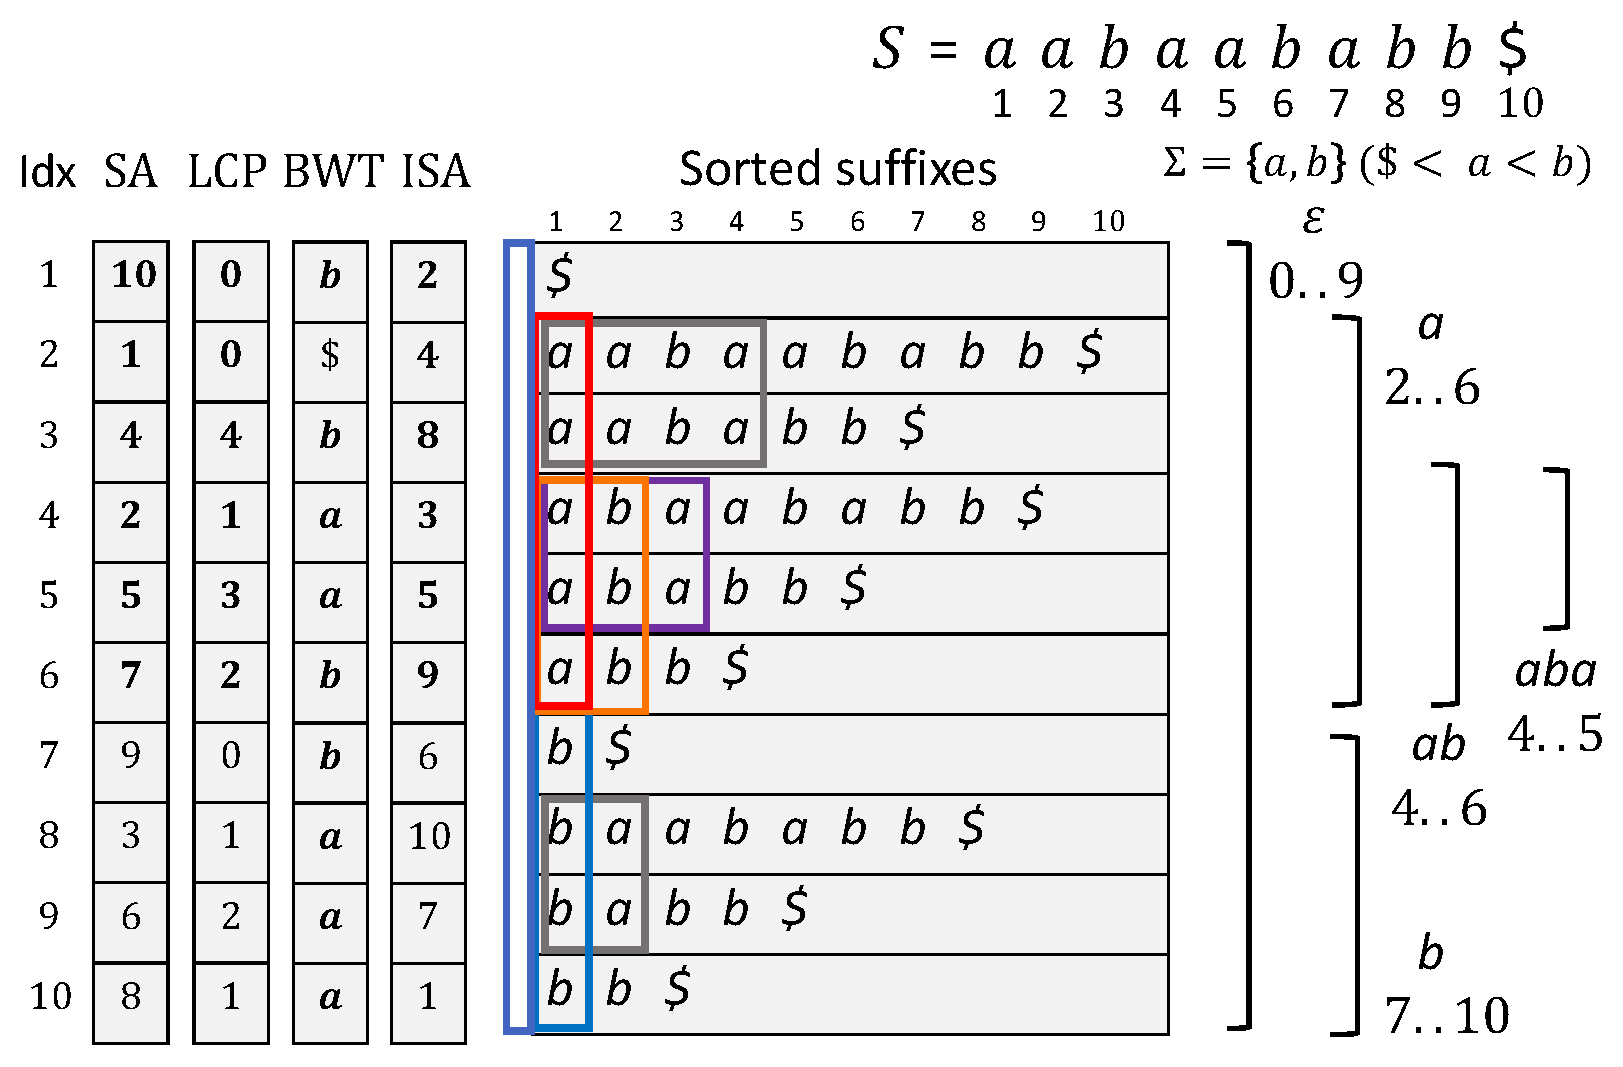
\includegraphics[width=0.70\textwidth]{fig1.pdf}
\vspace{.5\baselineskip}
\caption{An example of indexing arrays of a string $S[1..10] = aabaababb\daller$ of length $n = 10$ over alphabet $\Sigma = \set{a, b}$, whose index starts at $0$, where the left endmarker $S[0]=\#$ and the related suffixes are omitted. 
  Inside and to the right of the panel for sorted suffixes, each bold rectangle $R = [i..j]\times [0..\ell-1]$ and square bracket
indicate a rich representation $(i..j, \ell)$ of a repeat of $S$ and 
the associated SA-interval $i..j$, respectively. 
%% In the panel for sorted suffixes, each bold rectangle $R = [i..j]\times [0..\ell-1]$ in the panel indicates a rich representation $(i..j, \ell)$ of a repeat of $S$, while each square bracket indicates the associated SA-interval $i..j$. 
}\label{fig:example:arrays}
\end{figure}
%%%%%%

\subsection{Text indexing arrays}
%%\label{sec:prelim:ds:array}
Let $S[1..n-1]$ be a string of length $n-1$ and $\hat S[1..n] = S\cdot \daller$ be its extended string with endmarker $\daller \not\in \Sigma$. For any position , we denote by $\Suf[p] = S[p..n]$ the suffix of $S$ starting at position $\btw i1n$. 
We introduce a set of arrays for indexing a string as follows (see~\cite{navarro2016cds:book} for details).
We refer to lexicographic ranks as $i, k$ and positions as $p, q$.


The \textit{suffix array} $SA$ and \textit{inverse suffix array} $ISA$~\cite{manber:myers1993suffixarrays} are integer arrays defined as follows. 
The array $SA$ contains all suffixes of $\hat S[1..n]$ sorted in the increasing lexicographic order $<_\lex$ such that 
$S[SA[1]..n]<_\lex \dots <_\lex S[SA[n]..n]$. that is, $SA[k] = p$ means that $p = SA[k]$ is the starting position of the $k$-th rank in $<_\lex$ in $S$. 
Then, $ISA$ represents the inverse function of $SA$ such that $SA[ISA[p]] = p$ for all $p \in [n]$.

In the \textit{rich representation} on $SA$ array (see, e.g.\cite{kasai:lee2001lcp:linear,abouelhoda2004replacing}), we can uniquely encode any factor $w$ of a string $S$ by a triple $\tau = (i, j, \ell)$, denoted by $(i..j, \ell)$, such that
\begin{enumerate*}[(i)]
\item $i..j \subseteq 1..n$ is the SA-interval of $w$, i.e., $SA[i..j] = \Occ(w)$; and  
\item $\ell$ is the length of $w$, i.e., $\ell = |w|\ge 0$. 
\end{enumerate*}
Conversely, the rich representation $\tau = (i, j, \ell)$ can be decoded by the function $\getfactor(i..j, \ell) := S[p..SA[k]+\ell-1]$ using $\SA$ and $S$, where $\btw kij$ can be any rank in $i..j$. 

The \textit{longest common prefix array} $LCP[1..n]$ contains in the $k$-th rank the length of the longest common prefix of adjuscent suffixes $\Suf[SA[k-1]]$ and $\Suf[SA[k]]$ for all $k \in [n]$; We define $LCP[1] = 0$. It can be preprocessed in linear time supporting the \textit{range minima query} $RMQ_{LCP}(i, j)$ that, given $i\le j$, returns the minimum of $\set{\LCP[i], \LCP[i+1], \dots, \LCP[j]}$ in constant time and $O(n)$ space (Bender and Colton~\cite{bender:colton2000thelcaproblem}).
An example is shown in \cref{fig:example:arrays}. 

%%%
The \textit{Burrows-Wheeler Transformation} $\BWT[1..n]$ defines the permutation of a string $S$ by $BWT[k] = S[SA[k]-1]$ for all $k \in [2..n]$; We let $BWT[k] = \daller$ with $SA[k] = 1$~\cite{burrows:wheeler1994blocksorting}. 
%% For any $k \in [n]$, the \textit{LF-mapping} is defined by $LF(k) = ISA[n]$ if $SA[k]=1$ and $LF(k) = ISA[SA[k]-1]$ otherwise.
%%
It can be preprocessed in linear time in the \textit{Wavelet Tree} data structure (by~\cite{grossi2003high}) supporting the \textit{range distinct query} $RDQ_{BWT}(i, j)$ that, given $i\le j$, returns the set of mutually distinct characters in the range $BWT[i..j]$ in $O(\log\sigma)$ time and
linear space. 
%% $O(n/\log_\sigma n)$ space.
All the arrays can be constructed from $S$ in linear time over integer alphabet (see the textbook~\cite{navarro2016cds:book}). 


%% %%%%% 
%% \subsection{A concise representation of a substring}
%% \label{sec:triple}
%% We introduce a concise representation of a substring $W$ of a string $S$ with constant size, called the \textit{rich representation}, or simply a \textit{triple}, as follows~\cite{kasai:lee2001lcp:linear,ohlebusch2013bookbioinfo,belazzougui2015space:unusual}. 
%% Suppose that $SA \in [n]^n$ is the suffix array of $S$. Let $W \in Substr(S)$ be any substring of $S$. We can easily see that all ranks $k\in [1..n]$ whose starting positions $SA[k]$ belong to $\spos(W)$ occupy the contiguous subinterval $[L..R]\subseteq [1..n]$. We call this range $[L..R]$ the \textit{SA-range} of $W$.
%% We define the \textit{triple} for $W$ to be the integer triple $\tau = (L, R, \ell) \in [n]^3$, denoted $([L..R], \ell)$, such that $[L..R]$ is the SA-range of $W$ and $\ell = |W|$ is the length of $W$.
%% Conversely, $\tau$ \textit{defines} $W$ if $W = S[p..p+\ell-1]$ with $p = SA[L]$ is well-defined for some $k \in [L..R]$, and is unique. 
%% %%% 
%% For example, in \cref{tbl:arrays}, the substring $\mathtt{bc}$ has the triple $([7..9], 2)$ since it has the SA-range $[7,9]$ in $SA[1..13]$ and has the length $|W|=2$.


%% %%%% 
%% \mysubsubsection{Maximal repeats}
%% %%%%
%% To realize efficient enumeration of classes of unusual words, we use the class of maximal repeats of a string $S$, defined as follows.
%% Let $S = S[1..n] \in \Sigma^n$ be a string over alphabet $\Sigma$ and $\hat S[0..n+1] = \# S\daller \in \hat\Sigma^{n+2}$ be its extended version with endmarkers.
%% Let $u \in \Sigma+$ be any factor of $\hat S$. Since $\#, \daller \not\in \Sigma$, we see $u \in \Fac(S)$, namely, $u$ is contained in the content $S$.

%% \begin{definition}[maximal repeat]\rm 
%% A string $u \in \Sigma+$ is a \textit{maximal repeat} of $S$ if it satisfies conditions (1) and (2) below: 
%% \begin{enumerate}[(1)]
%% \item $u$ is a factor of $S$, i.e., $u \in \Fac(S)$. 
  
%% \item there exist two start positions $p, q \in \Spos[S](u)\;(p\not= q)$ of $u$ such that
%%   \begin{enumerate}[(i)]
%%   \item $u$ is \textit{left-branching} meaning that the preceding characters are mutually different, i.e., $S[p-1] \not= S[q-1]$, 
%%  and
%%   \item $u$ is \textit{right-branching} meaning that the following characters are mutually different, i.e., $S[p+|u|] \not= S[q+|u|]$. 
%%   \end{enumerate}
%% \end{enumerate}
%% \end{definition}

%% By definition, any maximal repeat $w$ occurs at least twice in $S$, that is, $w$ is a \textit{repeat} in $S$.
%% For later use, we define some notation: $\LSigma(u) \subseteq \Sigma$ (resp.~$\RSigma[](u)$) to be the sets of the preceding characters $S[p-1] \in \hat\Sigma$ (resp.~the following characters $S[p+|u|] \in \hat\Sigma$) by one over all positions $p\in \Spos(u)$ of $u$ in $\hat S$.
%% If it is clear from context, we write $\LSigma[](u)$ and $\RSigma[](u)$ for $\LSigma(u)$ and $\RSigma(u)$ by omitting subscript $\hat S$, respectively. 
%% In this notation, we see that a nonempty string $u$ is a maximal repeat of $S$ if and only if (1) $u \in \Fac(S)$ and (2) $|\LSigma(u)| \ge 2$ and $|\RSigma(u)| \ge 2$.


%% Now, we define the class of maximal repeats. 
%% %%are one of the most fundamental features in a string. 
%% Any subword $W$ of $S$ is called a \textit{repeat} if it occurs at least twice in $S$, namely, $\occ(W) \ge 2$.
%% A repeat $W$ is said to be \textit{left-branching} (resp.~\textit{right-branching}) in $S$ if either 
%% (i) $W$ is a prefix  of $S$ (resp.~a suffix of $S$), or 
%% (ii) there exist a pair of distict characters $a\not= b$ in $\Sigma$ such that $\occ(aW) \ge 1$ and $\occ(bW) \ge 1$ (resp.~$\occ(Wa) \ge 1$ and $\occ(Wb) \ge 1$).
%% A \textit{maximal repeat} is any repeat $W$ in $S$ that is both right-branching and left-branching in $S$. In what follows, $MR(S)$ denotes the set of all maximal repeats in $S$, and $\mu(S) = |MR(S)|$ denotes their number. 

%% A \textit{left-extension} (resp.~a \textit{right-extension}) of a maximal repeat $W \in MR(S)$ is any substring of $S$ in the form $cW$ (resp.~$Wc$) such that $\occ(cW)\ge 1$ for some $c \in \Sigma$. We denote by $e_L(S)$ (resp.~$e_R(S)$) the number of the left-extensions (resp.~right-extensions) in $S$. 
%% For a substring $W$ of $S$, $[W]^S_L = \sete{ U \in Substr(S) \mid \spos(U) = \spos(W) }$ denotes the equivalence class with the representative $W$, and $\rext W$ denotes the unique longest string in $[W]^S_L$. By symmetry, we can define the equivalence class $[W]^S_R$ and the representative $\lext W$  related to $\epos(W)$.
%% We often write, e.g., $e_L$ and $[W]_L$ for $e_L(S)$ and $[W]^S_L$, by omitting $S$. 

%% \begin{remark}
%% Weobserve the following properties: 
%% (i) for any repeat $W$, $\rext W$ is a right-branching repeat, while $\lext W$ is a left-branching repeat in $S$;
%% (ii) the operators $\set{\lext\cdot, \rext\cdot}$ are
%% %associative,
%% commutative and idenpotent.  
%% %the identities $\rext{(\lext W)} = \lext{(\rext W)} =: \mext W$,  $\lext{(\lext W)} = \lext W$, and  $\rext{(\rext W)} = \rext W$. 
%% (iii) a substring $U$ is a maximal repeat if and only if there exists a substring $W$ such that $U = \mext W := \rext{(\lext W)} = \lext{(\rext W)}$.
%% \end{remark}

%% Raffinot~\cite{raffinot2001maximal} found that the set $MR(S)$ coincides to the vertex set of the CDAWG~\cite{blumer1987complete} for a string $S$. 
%% Thus, $e_R$ satisfies $\mu \le e_R \le n$ and $\sigma \le e_R \le n$~\cite{blumer1987complete,raffinot2001maximal}. 
%% Belazzougui~\textit{et al.}~\cite{belazzougui:cunial:gagie:prezza:raffinot2015composite} have focused on $e_R$ as a fundamental repetitiveness measure related to $MR(S)$, and showed that $r \le e_R$ and $z \le e_R$. In general, $e_R = \Theta(n)$, while $e_R$ can be much smaller than $n$ for highly-repetitive strings. Radoszewski et al.~\cite{radoszewski:rytter2012structure:cdawg:thuemorse} showed that $e_R = O(\log n)$ for morphic strings, e.g.~Thue-Morse words.
 %% new 
% \section{Appendix}

\subsection{Related Work}

This section provides an overview of text indexing data structures related to this paper. 

\textbf{Text indexing data structures.} In 1973, Weiner \cite{weiner1973linear} proposed the suffix tree as a data structure for efficiently storing all substrings of a given text. He presented an algorithm to construct a suffix tree from a text of length n in $O(n \log n)$ time. A suffix tree has internal nodes corresponding to all right maximal repeats in the text and leaves corresponding to suffixes. Furthermore, he introduced the Weiner tree, a tree structure with the same vertex set as the suffix tree and consisting of the inverse links (called Weiner links) of the suffix links.
%% 
The CDAWG was proposed in 1987 by Blumer, Blumer, Ehrenfeucht, Haussler, and Mc-Connel~\cite{blumer1987complete}. Crochemore and Verin~\cite{crochemore:verin1997compact} gave in 1997 an offline linear-time construction algorithm for CDAWG. Inenaga \textit{et al.}~\cite{inenaga2005online} gave in 2005 an online linear-time construction algorithm for CDAWG.

The \textit{suffix array} is proposed by Manber and Myers~\cite{ManberM93:SA} in 1993, and independently by Gonnet, Baeza-Yates, and Snider~\cite{gonnet1992patarray} in 1992 under the name PAT-array, as a simple and space-efficient alternative to the suffix tree. Manber and Myers~\cite{ManberM93:SA} showed that the suffix array and the \textit{longest common prefix array} (LCP array) can be constructed simultaneously from a text in $O(n \log n)$ time. They presented an algorithm for searching for a substring of length m in $O(m+ \log n)$ time by combining the suffix array with the LCP array. The SA interval representation, a concise representation of substrings in a text, was initially used as an internal structure for pattern matching on suffix arrays.
The \textit{FM-index}, a text indexing structure was proposed by Ferragina and Manzini~\cite{Ferragina05:FM}, which consists of the Burrows–Wheeler transform (BWT) of a text and the Wavelet tree~\cite{grossi2003high}. 

\textbf{Traversal of a suffix tree using array structures.} Maximal repeats have been proposed by several authors as one of the fundamental techniques for enumerating substrings of a text. In 2001, Kasai, Lee, Arimura, Arikawa, and Park~\cite{kasai:lee2001lcp:linear} showed that the bottom-up traversal of a suffix tree can be simulated in $O(n)$ time and space by combining the suffix array, the inverse suffix array, and the longest common prefix array. In 2004, Abouelhoda, Kurtz, and Ohlebusch~\cite{abouelhoda2004replacing} showed that the top-down traversal of a suffix tree can be simulated in $O(n)$ time and space by combining the suffix array and the longest common prefix array. They called a data structure that combines the suffix array with various array structures an enhanced suffix array and demonstrated that many string processing problems that can be solved using suffix trees can also be solved using enhanced suffix arrays.
Beller, Berger, and Ohlebusch~\cite{beller:berger2012space:efficient:bbo} and Beller, Gog, Ohlebusch, and Schnattinger~\cite{bellergogohlebusch2013computing} in 2012 showed that the top-down traversal of the Weiner tree of a text can be simulated in $O(n)$ time and space using the FM-index, an index structure that combines the BWT array and the Wavelet tree data structure. This technique has become one of the fundamental techniques used in many subsequent algorithms for enumerating string features (See the textbook by Ohlebusch~\cite{ohlebusch2013bookbioinfo}).

\textbf{Enumeration of maximal repeats} has been extensively studied in the analysis of texts and genetic sequences (see the textbook by Gusfield~\cite{gusfield1997algorithms}). Gusfield~\cite[Section 7.12.1]{gusfield1997algorithms} gives a slightly complex algorithm for enumerating all maximal repeats using a suffix tree.
Raffinot~\cite{raffinot2001maximal} in 2001 showed first time that the set of all maximal repeats coincides with the set of the longest paths represented by the branching vertices of the CDAWG structure. Based on this characterization, he gave an algorithm for enumerating all maximal repeats in $O(n)$ time and space using the CDAWG.
Narisawa, Inenaga, Bannai, and Takeda (CPM 2007) gave an algorithm for enumerating all maximal repeats in $O(n)$ time and space by combining the suffix array, the inverse suffix array, and the longest common prefix array, based on the algorithm of Kasai \textit{et al.} for simulating the bottom-up traversal of a suffix tree.

Külekci and Vitter~\cite{kulekci2011efficient} in 2012 introduced the idea of combining the BWT array and the Wavelet tree structure and gave a memory-efficient algorithm for enumerating maximal repeats in $O(n \log n)$ time using this idea. Beller, Berger, Ohlebusch~\cite{beller:berger2012space:efficient:bbo}, and Schnattinger extended the algorithm of Beller \textit{et al.}~\cite{bellergogohlebusch2013computing} for simulating the top-down traversal of the Weiner tree and gave an algorithm for enumerating all maximal repeats in $O(n)$time and space using the BWT array and the Wavelet tree structure.
%%% 
In the context of compressed computation, Belazzougui, Cunial, K\"{a}rkk\"{a}inen, and M\"{a}kinen~\cite{belazzougui2020linear} in 2020 gave a compressed data structure (called the \textit{uni-directional BWT-index}) with $n \log\sigma + O(n)$ bits of space for enumerating various string features. They showed that by the depth-first traversal of the Weiner tree using this data structure, maximal repeats can be enumerated in $O(n)$ time with $O(\sigma^2 \log^2 n)$ bits of additional space.

\textbf{Relationship between our algorithms nad the previous work.} The two proposed algorithms in this paper combine existing traversal techniques extracted from the above existing algorithms with new ideas and implementations. The first $O(e_R)$ time enumeration algorithm is based on the idea of reducing the search space using the \textit{Weiner tree property}. Then, it achieves output-sensitive time complexity $O(e_L)$ by combining the \textit{top-down traversal} of the suffix tree using the suffix array and the LCP array by Abouelhoda \textit{et al.}~\cite{abouelhoda2004replacing} in 2004 and the \textit{$O(1)$ time left-branchingity test} by Narisawa \textit{et al.}~\cite{narisawa2007efficient} in 2007. 

On the other hand, the second $O(e_L \log n)$ time enumeration algorithm is an extension of the BBO algorithm based on the \textit{top-down traversal of the Weiner tree} with the BWT array, proposed by Beller \textit{et al.}~\cite{beller:berger2012space:efficient:bbo}, combined with \textit{$O(\log n)$ time maximal extension operation} with the suffix array, the inverse suffix array, and the longest common prefix array to make it output-sensitive. 

%%% EOF


\end{document}



% ---- Acq ----
%% \subsection*{Acknowledgments}
%% \medskip
%% \textbf{Acknowledgments.}\hspace{.5em}
%% The authors thank the anonymous reviewers for their comments which greatly improved this paper.
%% The first author is also grateful to Hideo Bannai for 
%% %%providing information on the literature
%% information on conversion between text indexes, and to Mitsuru Funakoshi for discussion on the sensitivity of text indexes. 
